%% This document gives an example on how to use the ntnumasterthesis
%% LaTeX document class.

%% Use short name MACS, MIS, CIMET, MTDMT, MIXD or MIS  
%% Language english or norsk
%% b5paper with oneside or twoside, you can set A4 if you want but you submit in b5

%% If you want print with the heading material on a4 paper you can use this format
%% \documentclass[MACS,english,a4paper,oneside,12pt]{ntnuthesis/ntnuthesis}

%% with the change to using DAIM we have a new option. include DAIM after english below removes the front page material so that you can then submit in the DAIM system. If you are wanting the front material remove DAIM and make sure you fill in the DaimData.tex file.
\documentclass[MIXD,english]{ntnuthesis/ntnuthesis}

\usepackage[T1]{fontenc}
\usepackage[utf8]{inputenc}     % For utf8 encoded .tex files allows norwegian characters in the files. This can be dangerous if you change to a differnt editor.
%\usepackage[pdftex]{graphicx, hyperref}   % For cross references in pdf
\usepackage{graphicx}
\usepackage{hyperref}   % For cross references in pdf


\usepackage{color}              % For colouring text 
\hypersetup{colorlinks=true,     
		linkcolor=blue,          % color of internal links (change box color with linkbordercolor)
    citecolor=blue,        % color of links to bibliography
    filecolor=blue,      % color of file links
    urlcolor=blue           % color of external links
		}
\usepackage{csvsimple}  % for simple table reading and display
\usepackage{url}
\usepackage{booktabs}
\usepackage{gnuplottex} %miktex option if using miktex on windows
\usepackage{rotating}
\usepackage{pdfpages}

\definecolor{darkgreen}{rgb}{0,0.5,0}
\definecolor{darkred}{rgb}{0.5,0.0,0}

\lstset{        basicstyle=\ttfamily,
                keywordstyle=\color{blue}\ttfamily,
                stringstyle=\color{darkred}\ttfamily,
                commentstyle=\color{darkgreen}\ttfamily,
}


%Typesetting of C++ but not always stable in titles etc...
\newcommand{\CPP}[0]{{C\nolinebreak[4]\hspace{-.1em}\raisebox{.1ex}{\small\bf +\hspace{-.1em}+\ }}}

%\usepackage[table]{xcolor}% http://ctan.org/pkg/xcolor
%\usepackage[nomessages]{fp}
%\newlength{\maxbarlen}


\newcommand\databar[3][gray!20]{%
  \FPeval\result{round(#3/#2:4)}%
  \rlap{\textcolor{#1}{\hspace*{\dimexpr-\tabcolsep+.5\arrayrulewidth}%
        \rule[-.05\ht\strutbox]{\result\maxbarlen}{.95\ht\strutbox}}}%
  \makebox[\dimexpr\maxbarlen-2\tabcolsep+\arrayrulewidth][r]{#3}}



\newcommand{\com}[1]{{\color{red}#1}} % supervisor comment
%\renewcommand{\com}[1]{} %remove starting % to remove supervisor comments
% This will appear in text \com{Lecuters comment} and be visible unless you uncomment
% the renewcommand line.

\newcommand{\todo}[1]{{\color{green}#1}} % items to do
%\renewcommand{\todo}[1]{} %remove starting % to remove items to do

\newcommand{\n}[1]{{\color{blue}#1}} % other comment
%\renewcommand{\n}[1]{} %remove starting % to remove notes

\newcommand{\dn}[1]{} % add the d to a note to say that you have finished with it.





% Set to true ONLY if using Harvard citation style
\newboolean{HarvardCitations}
\setboolean{HarvardCitations}{false} % false for computer science, true for interaction design and harvard style


\ifthenelse{\boolean{HarvardCitations}}{%
	\usepackage{natbib} % for Harvard names as citations.
}{%
	\usepackage[numbers]{natbib} % for Vancover numbers in bibliography
}

\newcommand{\q}[1]{\leavevmode\marginpar{\small\em #1}}
\renewcommand{\q}[1]{}


\begin{document}

% for students submitting in the DAIM system this information will not be used.
% their is an option for DAIM submission which removes this information and checks it is B5.
% Removing the DAIM option on the document type will use this material.

\setthesistitle{Leap Motion and free-hand gesture interaction - a screening tool for development delay}
\setthesisshorttitle{Leap motion based screening method} % a short version for the page headers if your normal title is too long to fit
\setthesisauthor{Susan Grundmann}
\setthesissupervisor{Assoc. Prof. Frode Volden}
%\setthesissupervisorA{Prof. Jon Yngve Hardeberg}  % if you have a second supervisor add it like this
%\setthesissupervisorB{Prof. Smart Guy}  % if you have a second supervisor add it like this


\nmtkeywords{Thesis, Latex, Template, IMT}
%\nmtdesc{This is the short description of a masters thesis}


\setthesisdate{01-06-2018}
\setthesisyear{2018}



%for CIMET theses you need to see all of these as well

%\setthesiscampus{Gj\o{}vik}
%\setthesisHostInstitution{\NTNU}
%\setthesisHostInstitution{University of Eastern Finland}
%\setthesisHostInstitution{Universit\'e Jean Monnet Saint-Etienne}

%\setthesisjuryA{} %jury names
%\setthesisjuryB{} %jury names
%\setthesisjuryC{} %jury names
%\setthesisjuryD{} %jury names


 % this is the file which contains all the details about your thesis
\makefrontpages % make the frontpages
\input{inc/mastersIntro}

\tableofcontents

\hypersetup{pageanchor=true}

% Comment with a percent to remove figures or tables:
\listoffigures
\listoftables
\lstlistoflistings

\chapter*{Abstract}
The topic of this master thesis covers the challenge with interactive freehand gestures in Human Computer Interaction.

summary
conclusion


The thesis describes the methodical approach of...


%This is a summary of the thesis including the conclusion of what was discovered.


\hypersetup{pageanchor=false}
%\chapter*{Acknowledgment}
I would like to thank .... for great help and motivation during my master thesis...... \ldots



\begin{flushright}
S.G.\\[1pc]

\end{flushright}
%\thesistitlepage % make the ordinary titlepage
\hypersetup{pageanchor=false}
%\include{summary}

\chapter*{Preface}

%Here, you give a brief introduction to your work. What it is (e.g., a Master's thesis in AIMT at NTNU, when it was carried out (e.g., during the autumn semester of 2021). If the project has been carried out with a company, you should mention this and also describe the cooperation with the company. You may also describe how the idea to the project was brought up.

%You should also specify the assumed background of the readers of this report (who are you writing for).\\[2cm]

This Master's thesis was written in conjunction with a part-time Master program in Interaction Design at Faculty of Architecture and Design at Norwegian University of Science and Technology, campus Gjøvik.\\%[1cm]

My motivation for this master thesis is a result of long standing passion for free-hand gesture interaction. Science fiction movie such as Iron Man or Minority Report inspired me and envisioned a new and exiting field in Human Computer Interaction.\\


I would like to thank my supervisor from NTNU Gjøvik, prof. Frode Volden, for his patience and great help during my master thesis. His expertise and feedback was crucial for the final result.\\

Furthermore, I would like to thank all parents who let me run the ability test on their children. Thank you for your cooperation and believing in my project. 
Also, I would like to thank the pediatrician, who, unfortunately, would liked to be anonymous,  for the short notice interview. I appreciate her opinion about the concept.\\

Additionally, I would like to thank Devinco, the company I am currently employed, for being understanding and supporting. I hope, I can contribute with useful ideas and expertise for all future work. Special thanks goes to Tore Sævik, head of department, for implanting the crazy idea to apply for higher education. Moreover, my dear colleagues, thank you for all support and motivation and help I got during my master thesis. \\

Last but not least, I would like to thank my closest friends, my family and especially my boyfriend for being so understanding for my all to often absence and listen to all my whining and frustration in the last months. Thank you for believing in me and for all motivation and contribution I have got. It was a hard and long journey and I am happy to finally have reached the goal. \\[2cm]


%\begin{center}
%\thesiscampus, 
\begin{flushright}

\thesisdate \\[1pc]
S.G.\\[1pc]
\end{flushright}
%\thesisauthor
%\end{center}
\chapter{Introduction}
\label{chap:introduction}


Conventional user interfaces in our time are mainly focusing on input from different devices such as mouse, keyboard or touchscreen. Many science fiction movies introduce the concept of gestural interaction on touch-less interfaces where hand and body motions perform one or other kind of actions to interact with the system. With the proliferation of mobile phones, motion tracking and sensor technology gestural interaction has become a subject of undergoing intense study. Researcher such as Montero et al claim that gestural interfaces are a more natural method of interaction (Montero et al., 2010). However, to what extend gestural interfaces are natural interactions is an issue where opinions are diverged greatly. Malizia and Norman for instance, stated that as long as people need to learn gesture command the interaction is not natural. The advantages are enormous in situations where natural manipulation is required, shortcut interactions are needed, a danger of distraction of visual attention and where interactions must be flexible because of various users (people with disabilities) and environments (Park and Han, 2014). Riener implied that research showed that gestural interactions decrease the cognitive and visual workload (Riener, 2012). Furthermore, as a relatively new modality, gestural interfaces seems to positively stimulate the feeling and behaviour of people and gives them joy and pleasure (Loehmann et al., 2013) (Ren et al., 2013). However, according to Freeman, gestural interfaces require the users full mental and physical attention (Dustin Freeman, 2012) and others researchers are even more skeptical. They believe that gestural interface are a step backward in usability of interfaces due to the lack of guidelines for gestural control. Interaction design principles such as visibility, consistency, discoverability, feedback and recovery are more or less absence  (Norman and Nielsen, 2010). Furthermore, the importance of social acceptance is also an issue that needs to be contemplated when designing gesture-based interfaces (Montero et al., 2010). Since there are no principles for gesture interfaces regarding social acceptance, researcher have proposed some guidelines including naturalness, unobtrusiveness and discreetness. (Montero et al., 2010) 
\newline
In order to develop useful gesture interface or gesture based systems, meaningful gestures are essential. However, not less important are suitable sensors that satisfy the requirements of the gesture-based system.
Gestural sensor technology is a growing industry and many various devices have been already developed. Oculus Rift\footnote{https://www.oculus.com/} for instance, is very popular and well known in the VR industry. Unfortunately, this device is quite pricey and it requires handhold devices to interact. However, there are other devices that able to record hand and body postures and gestures without any handhold aid.
These can be divided in wearable such as data-gloves (Gupta, Suwai) and hand-free such as Kinect and Leap Motion.
The question is whether those devices can be used in a medical context, specifically as a screening method for motor development. Nowadays, method for evaluating development delays are neither digital or computer based. A digital solution would decrease data processing time and be more reliable since the gained data is less subjective. Autism Spectrum Disorder is used as an example to illustrate potential application areas. Researchers such as Anzulewicz investigate the motor performance on children with ASD and she pointed out that there is a need computational system to measure motor-performance. 
\newline
To summarize, the aim of this study is to investigate whether hand-free interaction can be used as a new screening method for development delay in children.
\newline
The first step of the project is to gather general information. The literature review (chap. \ref{chap:background}) will enlighten the background theory in order to gain a deeper understanding of the topic. Additionally, the review will provide an insight of previous work done in this field. This will be the framework and guideline for the other chapter where the aim of the study is elaborated and research questions and hypotheses are formulated. The method chapter (chap. \ref{chap:methods}) describes the process of designing the prove of principles, the approach and materials that were used during the design process. The gathered data is then presented and analyzed in chapter \ref{chap:dataanalysis}. Finally, the findings are compared with the theory from chapter \ref{chap:background} and discussed further in the discussion chapter (\ref{chap:discussion}). The discussion will enlighten whether the hypotheses can be confirmed or whether it must be refuted.


%what is the topic
%Explain why this topic is important
%brief summary of previous work
%outlines the purpose
%raod map> contents of each chap
%!Never put any results or decisions in the Introduction!

%things to mention in intro
%motor performance delay e.g. in asd
%touch-free sensors
%development screening methods
%performance measure
%gesture interfaces
%gesture interction


%To develop a gesture interface, we need some criteria to evaluate its performance,such as: meaningful gestures; suitable sensors; efficient training algorithms; and accurate,efficient, on-line/real-time recognition. 
%the aim of the study is to..

\section{Justification, motivation and benefits}
Gestural touch-less interfaces as a relatively new form of interaction is an exciting field of study. Using this new form of interaction in health care and medical science can open doors for new ideas and possibilities. For that reason it is worth to investigate the feasibility of creating a gesture based system to extract parameters which can be processed and analyzed in order to detect deviation from normal motor development in children. Data gained during the analyzing process could than be used as an indicator for development delays such as in Autism Spectrum Disorder.
Moreover, if the study reveals that a portable device such as Leap Motion is suitable for extracting important parameter regarding development delays then it might be an interesting and affordable alternative to nowadays screening methods.



 % includes latex files from the same directory
%\include{inc/packages} % could be called Methodology or methods or any filename 
%\include{inc/structure} % could be results
%\include{inc/implementation}
%\chapter{Methods, approach and materials}
\label{chap:methods}


\section{Interview}
\label{sec:interview}
Interviews are an essential part for each research. In order to gain a deeper understanding and a good overview regarding ASD test and screening methods for autism, interviews with medical - and child care personnel were planned. Additionally, information about the assessment of motor coordination skills used in Norway and Germany were of great importance.
Surprisingly, it was quite challenging to find people who have some kind of experience in the field of ASD. It seemed that only specialist in psychology could provide professional and deeper background information. For that reason, the interviews in this study were only in form of a brief conversation. However, the information gained during those conversations was useful and enlightening.


\subsection{Summary and conclusion of the interviews}

The interviewees provided insights in how Autism is handled in school environment and in context with ergo-therapy.  

The conversations revealed that children usually are not tested for Autism in preschool, however in case of observed abnormalities they will talk to the parents and recommend a further investigation with a psychologist specialized in child behaviour and development. Abnormal behaviour of children is characterized by language delay, dislike of body contact, dislike of noise and difficulties in understanding face mimic.
Additionally, the conversation also revealed that screening routines for children that could discover deficit as for instance autism is in general not carried out due to the poor time capacity and cost.
On the other hand, an ergo-therapist explained that it is hard to detect autism by testing fine-motor performance. However, children with autism would have problems to understand a certain task or game rules. Furthermore, receptive behaviour is also an distinguish sign for autism.
She also mentioned the problem with poor empathy and recognition of facial expression.

To conclude, evaluation of children's motor performance may not be a sufficient approach in order to discover Autism. Many other factors need to be considered when dealing with this problem. 



\section{Game design, prototype and limitation}
\label{sec:prototype}


\subsection{Leap Motion Device}

The Leap Motion device was purchased second hand on Finn. \footnote{www.finn.no} The V2 desktop tracking installation files which included the SDK version v2.3.1 were downloaded from Leap Motion website. \footnote{ www.leapmotion.com} The installation was straightforward and the device could immediately be connected to the PC and used with the Leap Motion visualizer.

\begin{figure}[h]  %t top, b bottom, p page | you can also use h to try to get the figure to appear at the current location
  \centering
  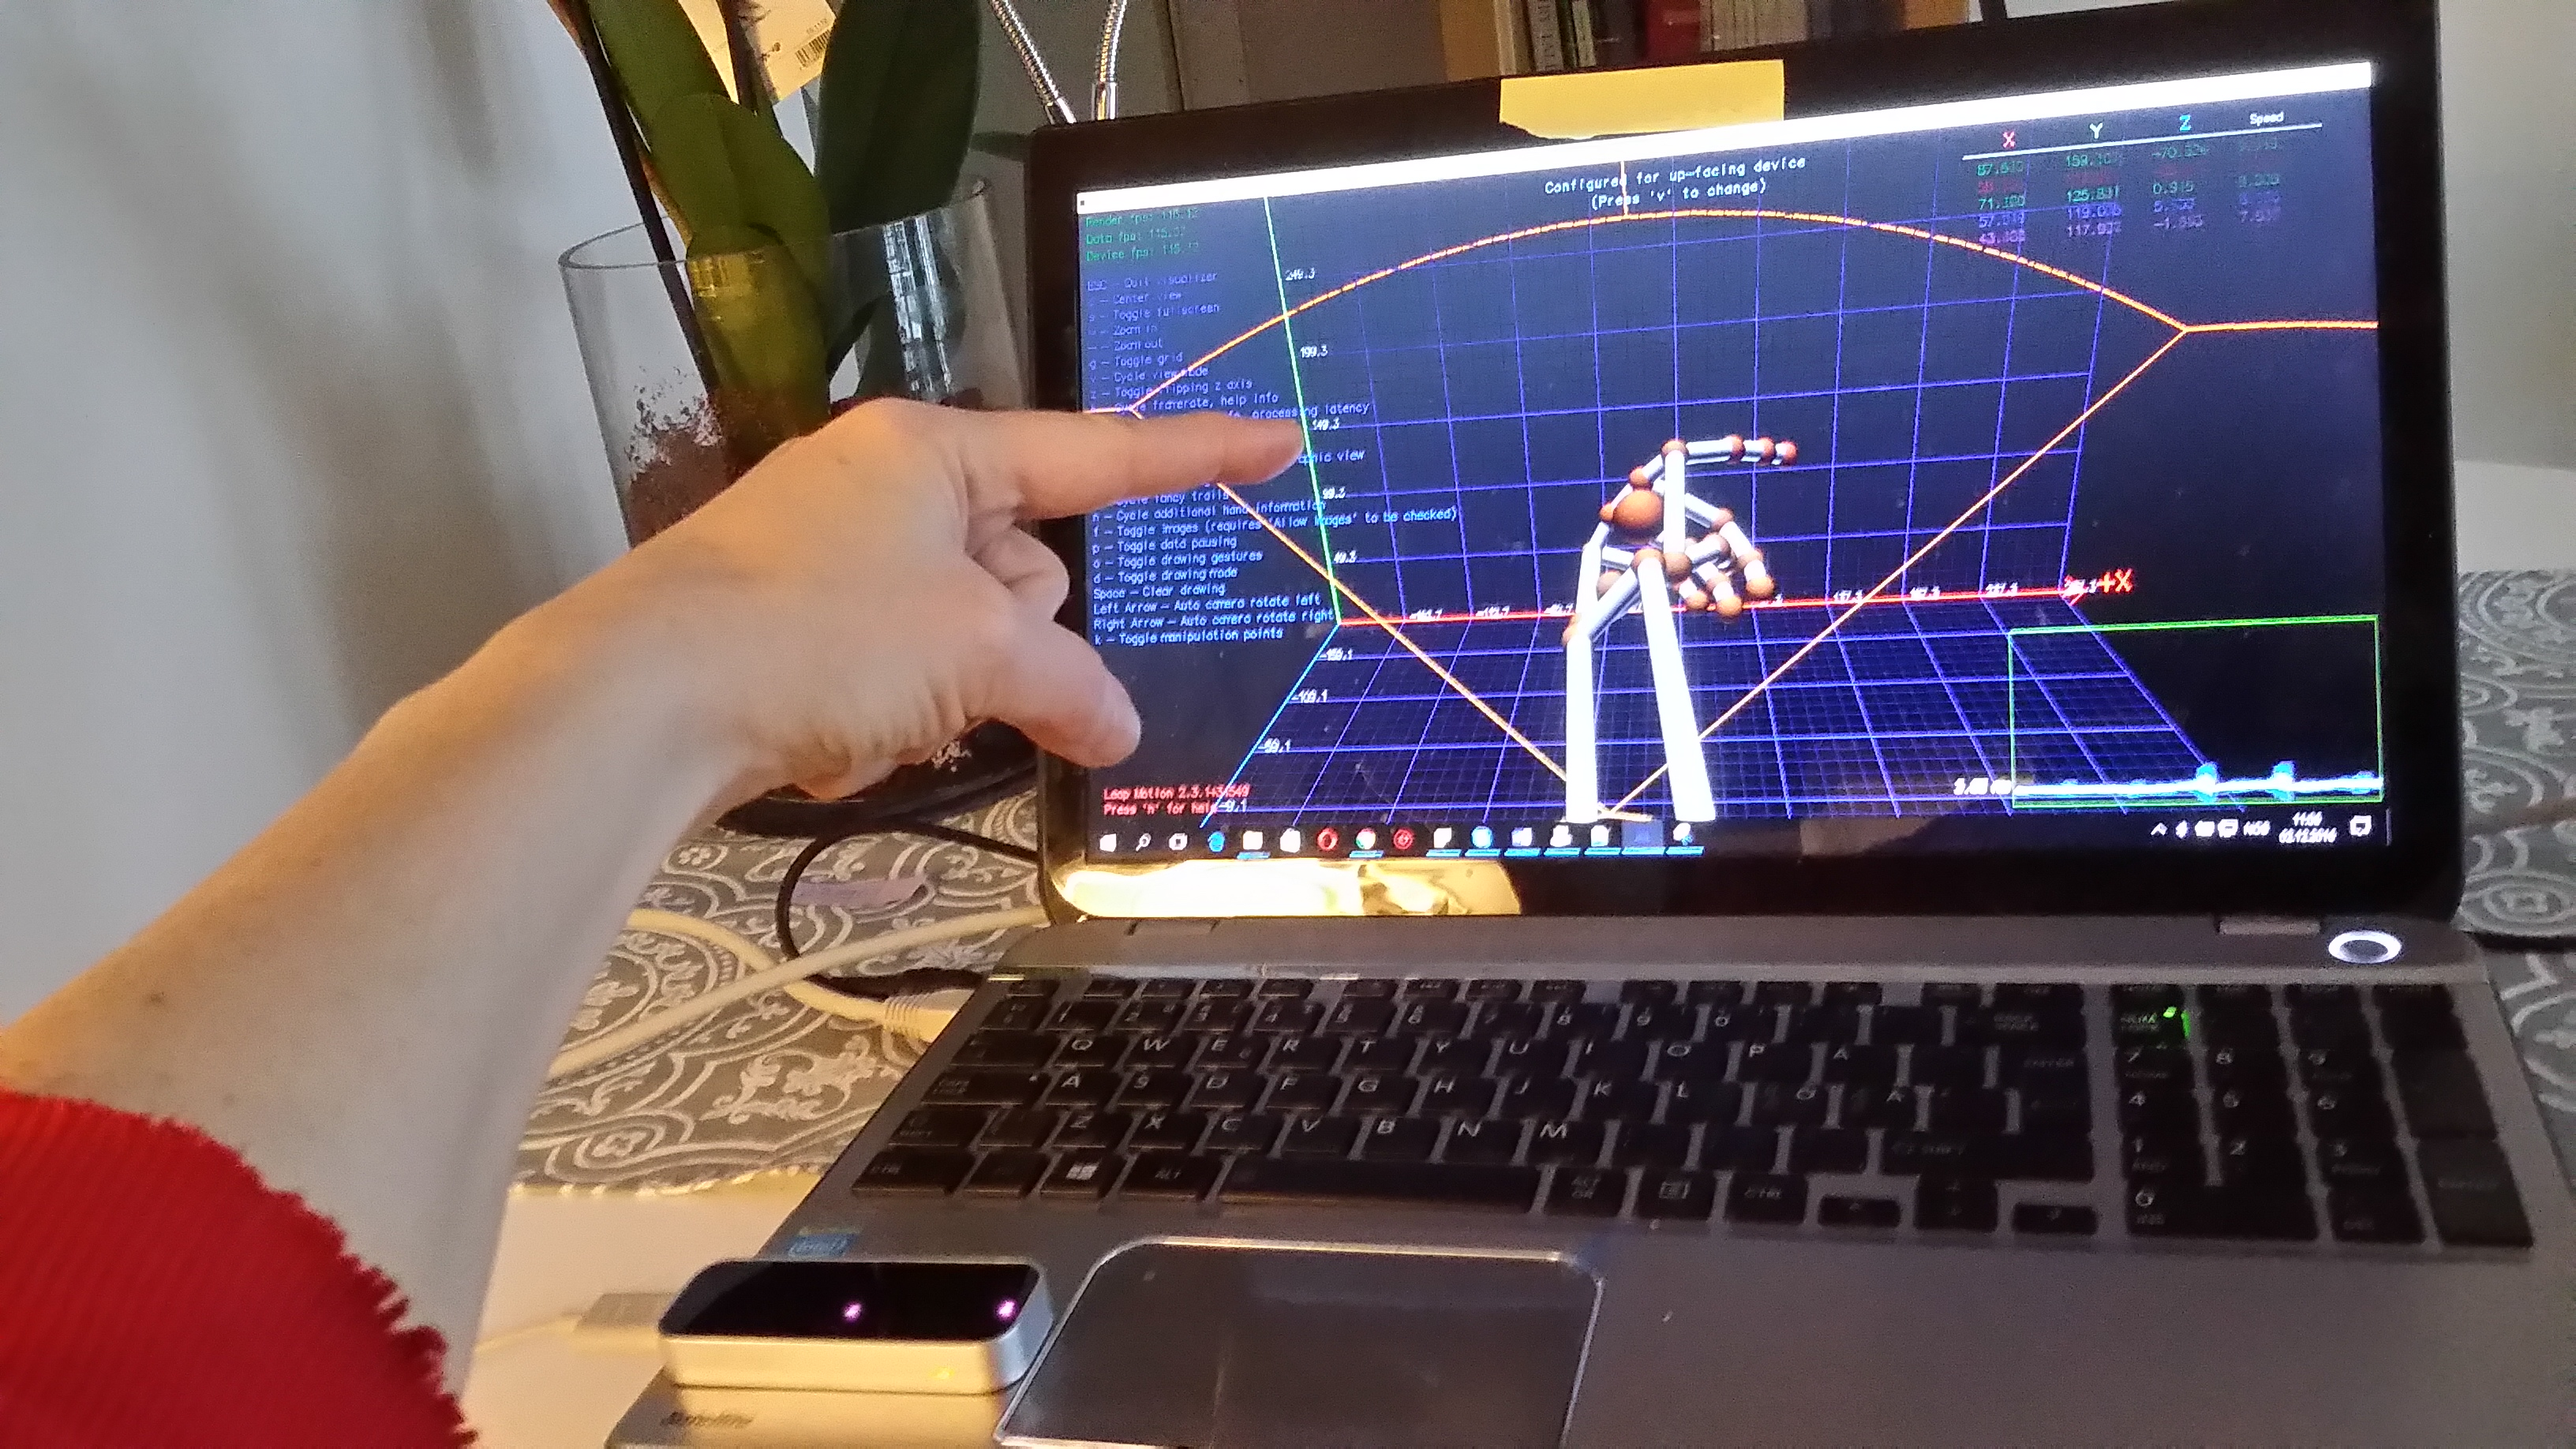
\includegraphics[width=.5\textwidth]{figures/LMvisualizer.jpg}
  \caption[Leap Motion visualizer.]{Leap Motion visualizer.}
  \label{fig:setup}
\end{figure}

The Java SDK documentation provided a good overview of the tracking data, hardware and software and showed how to get started with the Leap Motion API which was an excellent help during the whole prototyping process.

\subsection{Choosing a prototype tool}

A software prototype for test purpose was necessary to develop for this project. In order to accomplish the task it was essential to find a tool that could be used to create a simple and fast prototype and additionally is compatible with the Leap motion sensor. A quick Google search suggested Processing \footnote{https://processing.org/} which is a free open-source software. According to processing.org, the software is built particular within visual arts but also used for animation, installation products and interactive experience. It is a convenient prototype tool because it contains a integrated graphical user interface and additionally it is possible to use Java programming language in a simplified form.
Processing could also be used as a bridge between Leap Motion and Eclipse \footnote{https://eclipse.org/} which is known as an essential tool for Java developer.  Nevertheless, using Eclipse would be extensive and the setup would be more time consuming even if this would have been a more professional approach.

However, for this project, a simple and fast prototype was completely sufficient. For that reason, Processing was a suitable option. For the prototype development, Processing version 3.3.6 was installed locally.


\subsection{Game design}

In the initial design stage the idea of the whole system was sketched. In this stage the system had five modules. However, only one module could be implemented for this project due to the time limit.

\begin{figure}[h]  %t top, b bottom, p page | you can also use h to try to get the figure to appear at the current location
  \centering
  \includegraphics[width=.6\textwidth]{figures/sketch_wholeSystem.jpg}
  \caption[Idea generating.]{ Idea generating for the whole system}
  \label{fig:setup}
\end{figure}

For this project, the module "Mole in the hole" was chosen to implement further.

\begin{figure}[!h]  %t top, b bottom, p page | you can also use h to try to get the figure to appear at the current location
  \centering
  \includegraphics[width=.6\textwidth]{figures/prototypeSketch.jpg}
  \caption[Sketch Mole in the hole.]{Sketch: Mole in the hole}
  \label{fig:setup}
\end{figure}

At the second stage of the design process the background picture and figures needed to be created.The background picture was created in Adobe illustrator, version CS4. A photo illustrating the forest floor was downloaded free from Pixaby \footnote{www.pixaby.com} and used for the upper part of the game’s canvas. The underground was drawn as a vector art to make it more childlike. 
A grid was drawn and used as dimension and measurement aid for the white path. This was needed to simplify the programming implementation that used the same grid size. However, the grid was just an drawing aid and was not visible in the end product.

\begin{figure}[h]  %t top, b bottom, p page | you can also use h to try to get the figure to appear at the current location
  \centering
  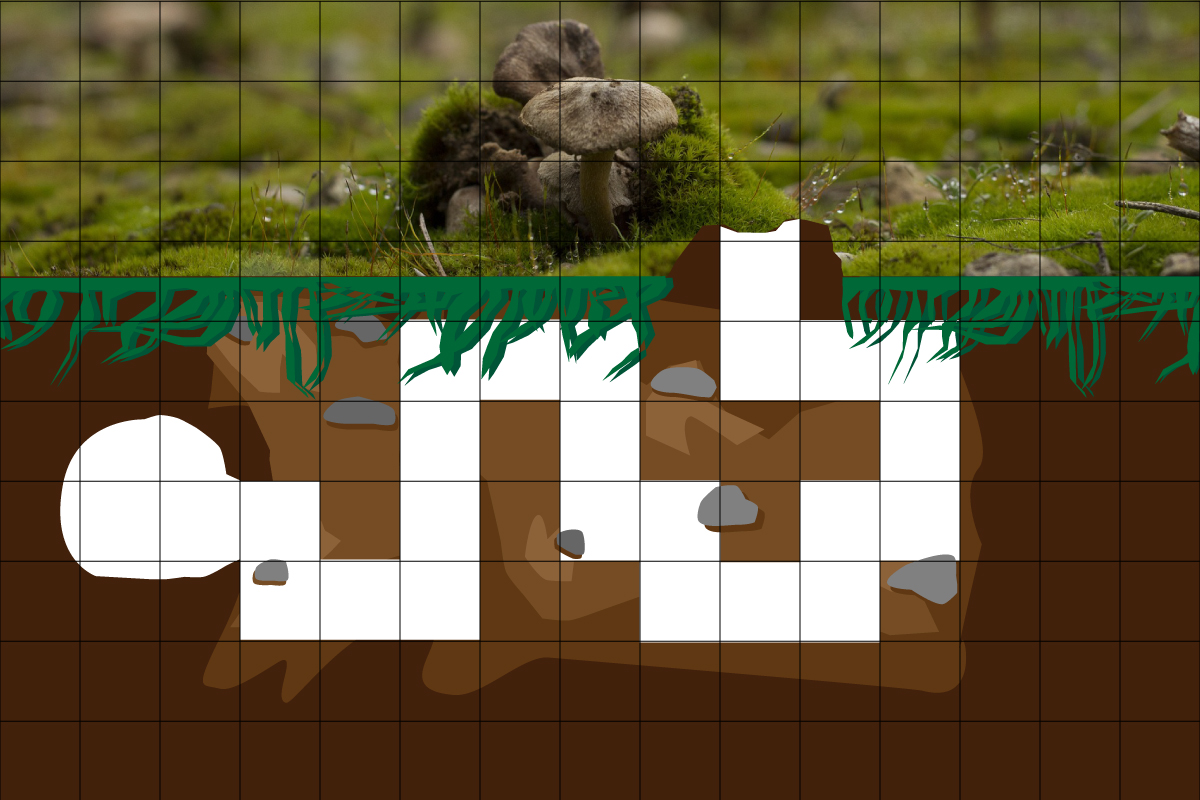
\includegraphics[width=.5\textwidth]{figures/Mole-in-the-hole-800x1200-GRID.jpg}
  \caption[Mole in the hole grid.]{Mole in the hole - grid.}
  \label{fig:setup}
\end{figure}

The five mole states and the stopwatch were drawn as a vector graphic in Adobe Illustrator, as well.

\begin{figure}[h]  %t top, b bottom, p page | you can also use h to try to get the figure to appear at the current location
  \centering
  
\includegraphics[width=.1\textwidth]{figures/MoleWait.png}
   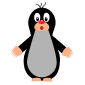
\includegraphics[width=.1\textwidth]{figures/MoleAttention.png}
   
\includegraphics[width=.1\textwidth]{figures/MoleJump.png}
   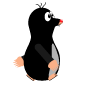
\includegraphics[width=.1\textwidth]{figures/MoleGo.png}
   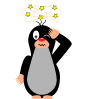
\includegraphics[width=.1\textwidth]{figures/MoleKaBoom.png}
  \caption[Mole's states.]{ The Mole's states: wait, attention, ready, go, hit.}
  \label{fig:setup}
\end{figure}

\begin{figure}[h]
  \centering
  
\includegraphics[width=.1\textwidth]{figures/timer.png}
  \caption[Timer]{Timer}
\end{figure}


The third design stage focused on illustrating the implementation and demonstrated the solution to the given problem.
A flow diagram was created for a better understanding of the design process and to analyze design problems. It illustrates the process stages and the conditions during the process from start point to the end point. 

\break

\begin{figure}[h]
    \centering
    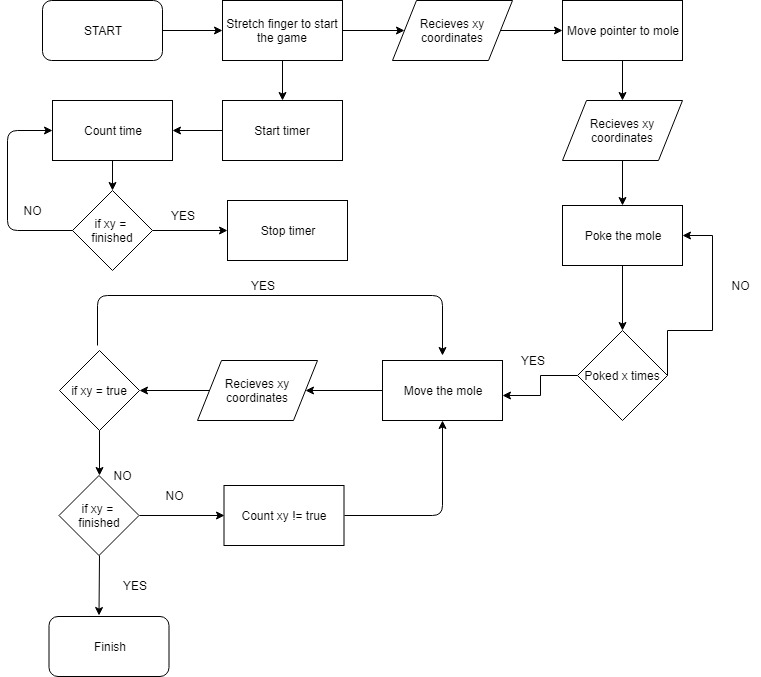
\includegraphics[width=.8\textwidth]{figures/FlowDiagram.jpg}
    \caption[Flow diagram: game design]{Flow diagram illustrates the game process}
    \label{fig: flowdiagram}
\end{figure}


\subsection{Prototype implementation}

In Processing, in order to make an animation or a interactive program, a predefined structure is used which includes a setup() and a draw() function. The setup() function runs only ones at the start whereas the draw() function loops continuously until the program is terminated or the noLoop() command appears in the code.
In the setup() function, the initial environment property as for instance the size of the canvas is defined  (size()).  In the draw() function, code that is meant to run continuously is defined here, like for instance the background() property. 

The framework would look likes this:
\lstset{frameround=tttt}
\lstset{frame=single}
\lstset{xleftmargin=.05\textwidth, xrightmargin=.05\textwidth}
\lstset{language=Java}
\begin{lstlisting}[caption = {Processing framework}, label={lst:Java}]
        void setup(
        {
            size();
        }
        void draw()
        {
            background();
        }

\end{lstlisting}

The program code for the module “Mole in the hole” implemented functions from the Leap Motion API. In order to use these functions the leap Motion library needed to be imported.

\lstset{language=Java}
\begin{lstlisting}[caption = {Leap Motion library}, label={lst:Java}]
import com.leapmotion.leap.*;
\end{lstlisting}

To connect to the Leap motion device a controller object was created

\lstset{language=Java}
\begin{lstlisting}[caption = {The code for touch zone}, label={lst:Java}]
Controller leap;
\end{lstlisting}

In setup() the controller was initialized as followed in order to establish a connection.

\lstset{language=Java}
\begin{lstlisting}[caption = {The code for touch zone}, label={lst:Java}]
leap = new Controller();
\end{lstlisting}

In order to make it easier to map position in the Leap Motion coordinate system an interaction box was initialized. The position within the 2D coordinate system was defined as X, Y which are coordinates for the hand and finger position. 

\lstset{language=Java}
\lstset{breaklines=true,postbreak=\mbox{{\color{blue}\tiny$\rightarrow$}}}
\begin{lstlisting}[caption = {The code for touch zone}, label={lst:Java}]

InteractionBox iBox = leap.frame().interactionBox();
Pointable pointable = leap.frame().pointables().frontmost();
Vector normalizedPosition = iBox.normalizePoint(pointable.stabilizedTipPosition());
float pixelX = normalizedPosition.getX() * windowWidth;
float pixelY = windowHeight - normalizedPosition.getY() * windowHeight;
int cx = (int) pixelX - 10;
int cy = (int) pixelY - 100;

\end{lstlisting}

Finger are recognize by the pointable class. The pointable.Zone defines the state of the current pointable object.

\lstset{language=Java}
\begin{lstlisting}[caption = {The code for touch zone}, label={lst:Java}]
 Pointable.Zone fingerzone = pointable.touchZone();
\end{lstlisting}

The touch zone is defined by three states:(see Leap Motion API reference for more information)
\begin{enumerate}
    \item ZONE\_NONE (pointable distant from the touch panel)
    \item ZONE\_HOVERING (is near the touch plane)
    \item ZONE\_TOUCHING (penetrates the touch plane)
\end{enumerate}




\lstset{language=Java}
\begin{lstlisting}[caption = {The code for touch zone}, label={lst:Java}]

            switch (pointable.touchZone()){
            case ZONE_NONE:
              //Handle distant pointable
              image(MoleState1, 80, 480);
              break;
            case ZONE_HOVERING:
              //Handle pointable near touch plane
              hide(MoleState1);
              image(MoleState2, 80, 480);
              break;
            case ZONE_TOUCHING:
              //Handle pointable penetrating touch plane
              counterTouching = counterTouching + 1;
              image(MoleJump, 80, 480); 
              break;
            default:
              //Handle error cases...
              break;
            }//end switch
          
\end{lstlisting}

A new finger object is created and initialized that starts the timer:

\lstset{language=Java}
\begin{lstlisting}[caption = {The code for touch zone}, label={lst:Java}]
  Finger finger = new Finger(pointable);
  if(finger.isExtended())
  {
    Timer(1);
  }
\end{lstlisting}

\break
%\break
In this game an invisible grid was drawn over the whole canvas size. Each grid cell had a size of 80 x 80 px. The mole’s hole and the way out was marked with white cells which x-y coordinates were stored as true-value in a two dimensional array.

\begin{figure}[h]  %t top, b bottom, p page | you can also use h to try to get the figure to appear at the current location
  \centering
  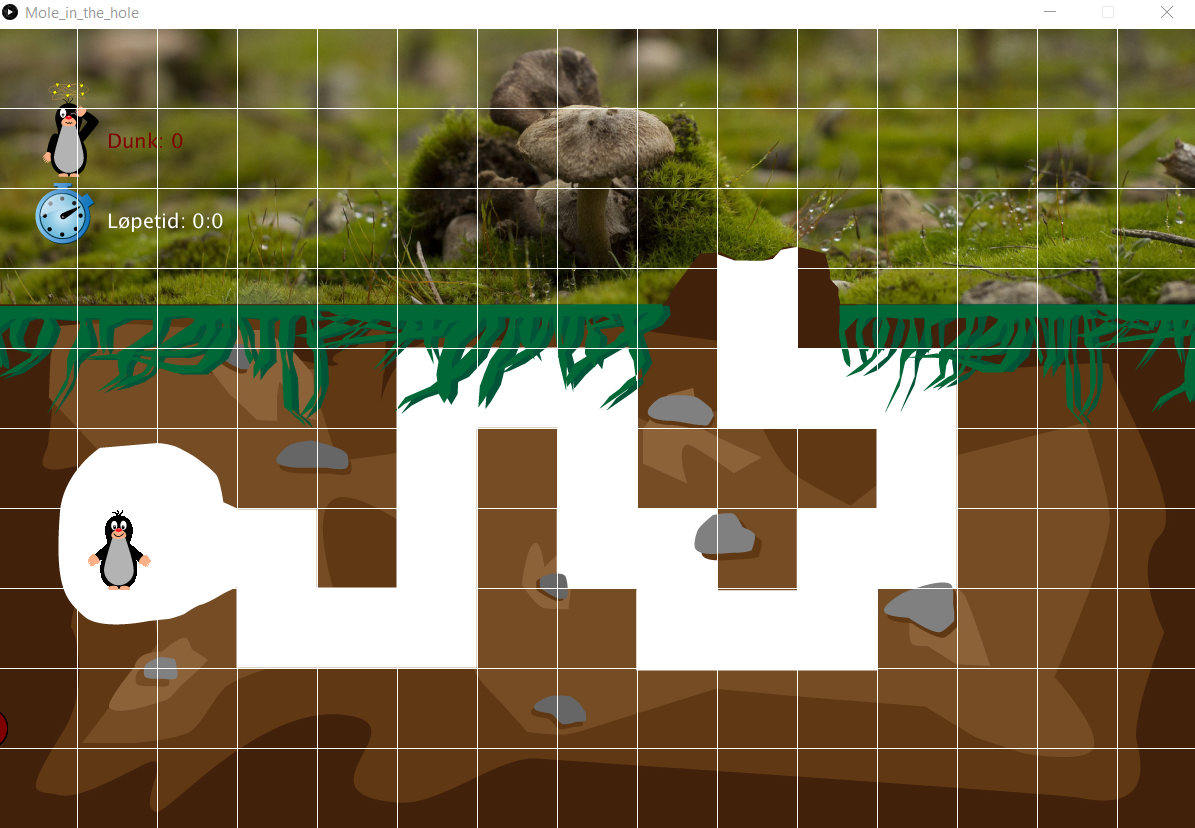
\includegraphics[width=.5\textwidth]{figures/Grid-processing-Mole_in_the_hole.png}
  \caption[Mole in the hole grid processing.]{Mole in the hole. Grid is drawn with a for loop.}
  \label{fig:setup}
\end{figure}

The pointer is activated by stretching the finger and pointing forward. The point moves in relation to the finger’s x,y coordinate. When the pointer hovers the mole, the mole changes state from “wait” to “attention”. When the Hole is poked his state will change from “attention” to “ready”. It needs about two til three pokes until the mole state changes to “go”. From that point the pointer disappear and only the mole moves and follows the finger’s position. All moves that are defined as false are counted as “hit”. The games is finished when the mole reaches the exit. The game counts the amount of hits and the elapsed time. The timer starts when the finger is stretched and the participant is ready to go.

\begin{figure}[h]  %t top, b bottom, p page | you can also use h to try to get the figure to appear at the current location
  \centering
  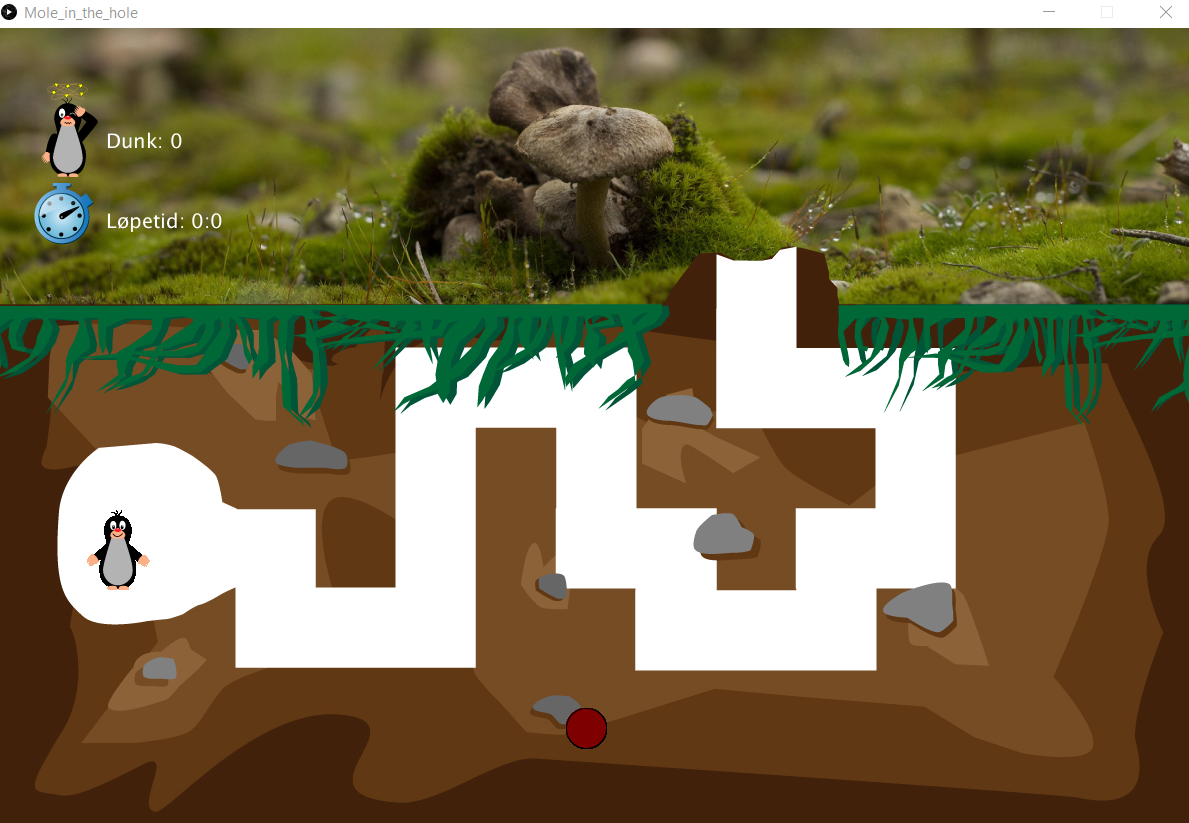
\includegraphics[width=.5\textwidth]{figures/StateStart-Mole_in_the_hole.png}
  \caption[Mole in the hole state start.]{Mole in the hole. State: start.}
  \label{fig:setup}
\end{figure}
\begin{figure}[h]  %t top, b bottom, p page | you can also use h to try to get the figure to appear at the current location
  \centering
  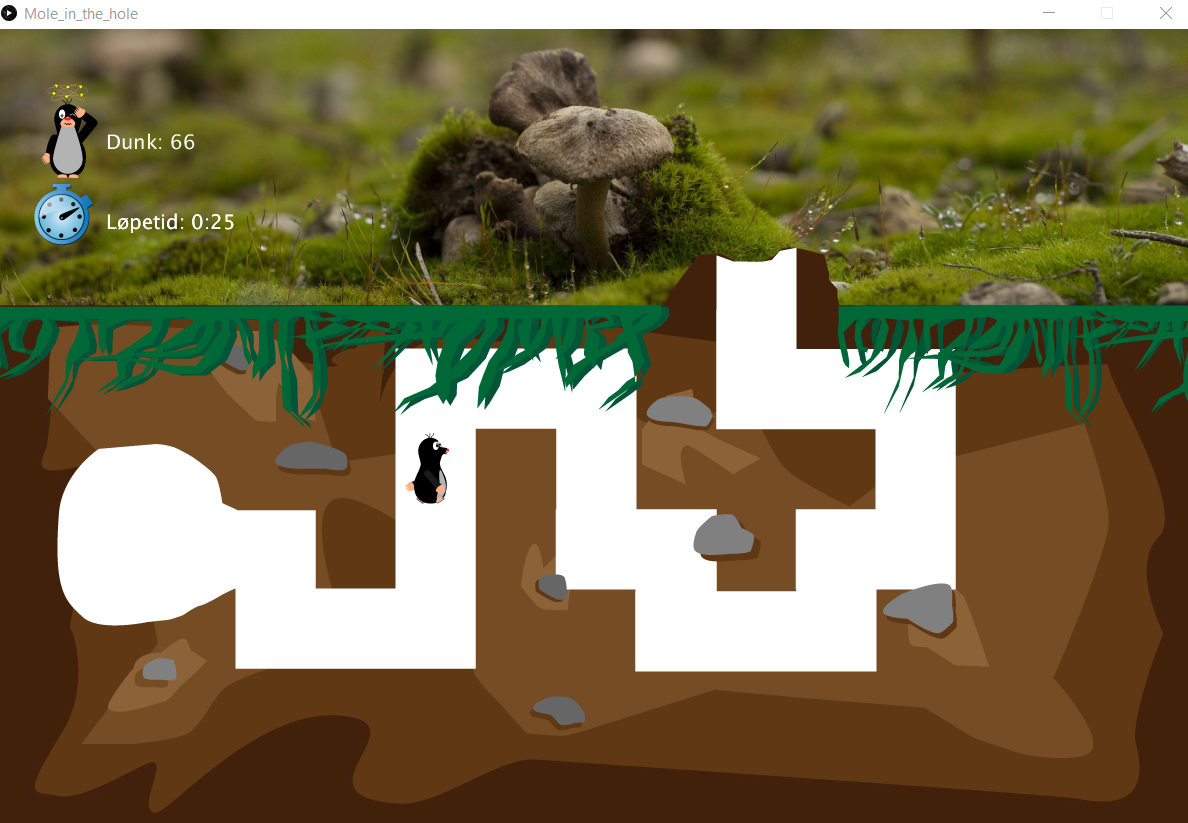
\includegraphics[width=.5\textwidth]{figures/StateGo-Mole_in_the_hole.png}
  \caption[Mole in the hole state go.]{Mole in the hole. State: go.}
  \label{fig:setup}
\end{figure}
\begin{figure}[h]  %t top, b bottom, p page | you can also use h to try to get the figure to appear at the current location
  \centering
  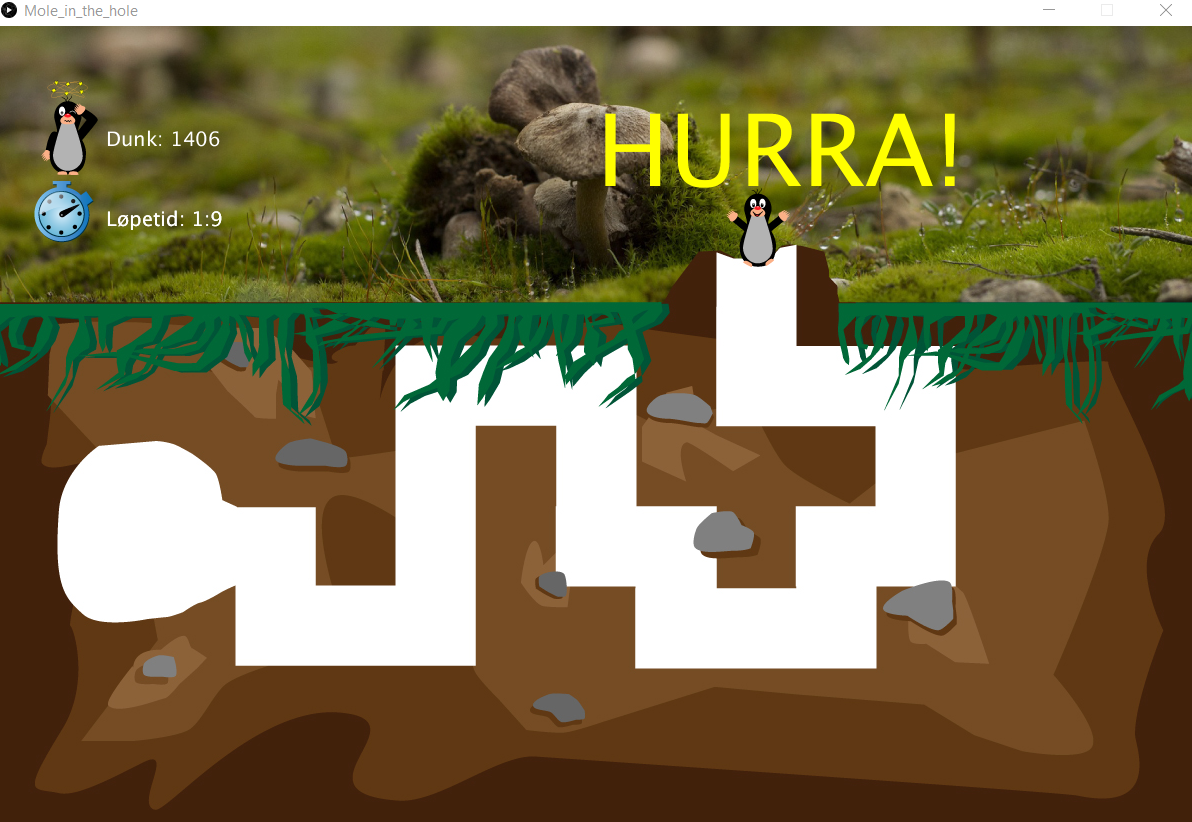
\includegraphics[width=.5\textwidth]{figures/EndState_Mole_in_the_hole.png}
  \caption[Mole in the hole state end.]{Mole in the hole. State: end.}
  \label{fig:setup}
\end{figure}



\subsection{Limitation}
time limit
money? budget
poor code quality
equipment limitation

\section{Experiment }
\label{sec:experiment}


\subsection{Recruiting participant}
\label{sec:participant}

The target group for this study were children between two and 13 years of age. A suitable combination of gender distribution would be appropriate for the usability test. For this purpose, convenience sampling of children that were readily available represent a subset of the population. A social network as recruiting source was substantial in this situation. Parents who saw the value of this study wanted to contribute and volunteered their children. 
The motive behind such young target group is, to observe and analyze if the child understands the idea a touch-less system and the ability to handle it. 

According to www.usertest.com, it is recommend to divide children into specific age groups. The main reason for that is the remarkable differences in development of cognitive, physical and social skills. For instance, fine-motor skill are less developed in a 3 year old child than i an a 10 year old. The user group in this study can be divided into group 1 (age 2 - 4), group 2 (age 5 - 8) and group 3 (age 9 -1).

The planed number of participant for the usability study was between nine and ten children. Since the study focused on qualitative data collection and Nielsen recommends 5 users for usability test, the amount of users were sufficient for this study. That would be a sufficient backup in case a child did not want to cooperate or if a child got ill. 


\subsection{Test environment and implementation strategy}
\label{sec:environmnent}

The project is about gaining meaningful data from a gesture-based application when screening children for fine motor deficiency
Working with children can be fun but also challenging at the same time. It needs a certain sensitivity and understanding of children's behaviour and feelings. Children can feel insecure  and anxious in a new environment which could make testing more stressful which probably would result in a wrong outcome. For that reason, each test was conducted at the child's home - a familiar and save environment. Since the equipment was portable, changing the test environment for each participant was not a concern.
Furthermore, in order to gain meaningful data from the experiment, a child's cooperation was necessary.  After a long day at daycare or at school, kids are usually tired and unfocused and hard to motivate. That is especially the case of younger children. For that reason, the experiments were carried out during the weekend and public holidays.  

The time duration needed to complete the task was estimated to 15 minutes. That included 3 attempts and answering the follow up questions. Additionally, extra 20 - 30 minutes were planned for presentation, introduction, equipment setup, debriefing and final thank-you-conversation.

\subsection{Compensation}

According to Nielsen [1998], compensating test users is common. The value of the compensation depends on the type of study and participants. However, he suggested a nice toy or 10 - 15\$ for children or students.
In this study, every child got a small compensation for their contribution. A collection of toys, games, book and other things were offered to choose from. This showed to be a good motivational tool and the children were eagerly to participate and accomplished the task.  

https://www.nngroup.com/articles/when-to-outsource-recruiting-test-users/



\subsection{Equipment}

The equipment for the experiment consisted of a laptop, an external screen and a gesture sensor (Leap Motion). 

\begin{figure}[h]  %t top, b bottom, p page | you can also use h to try to get the figure to appear at the current location
  \centering
  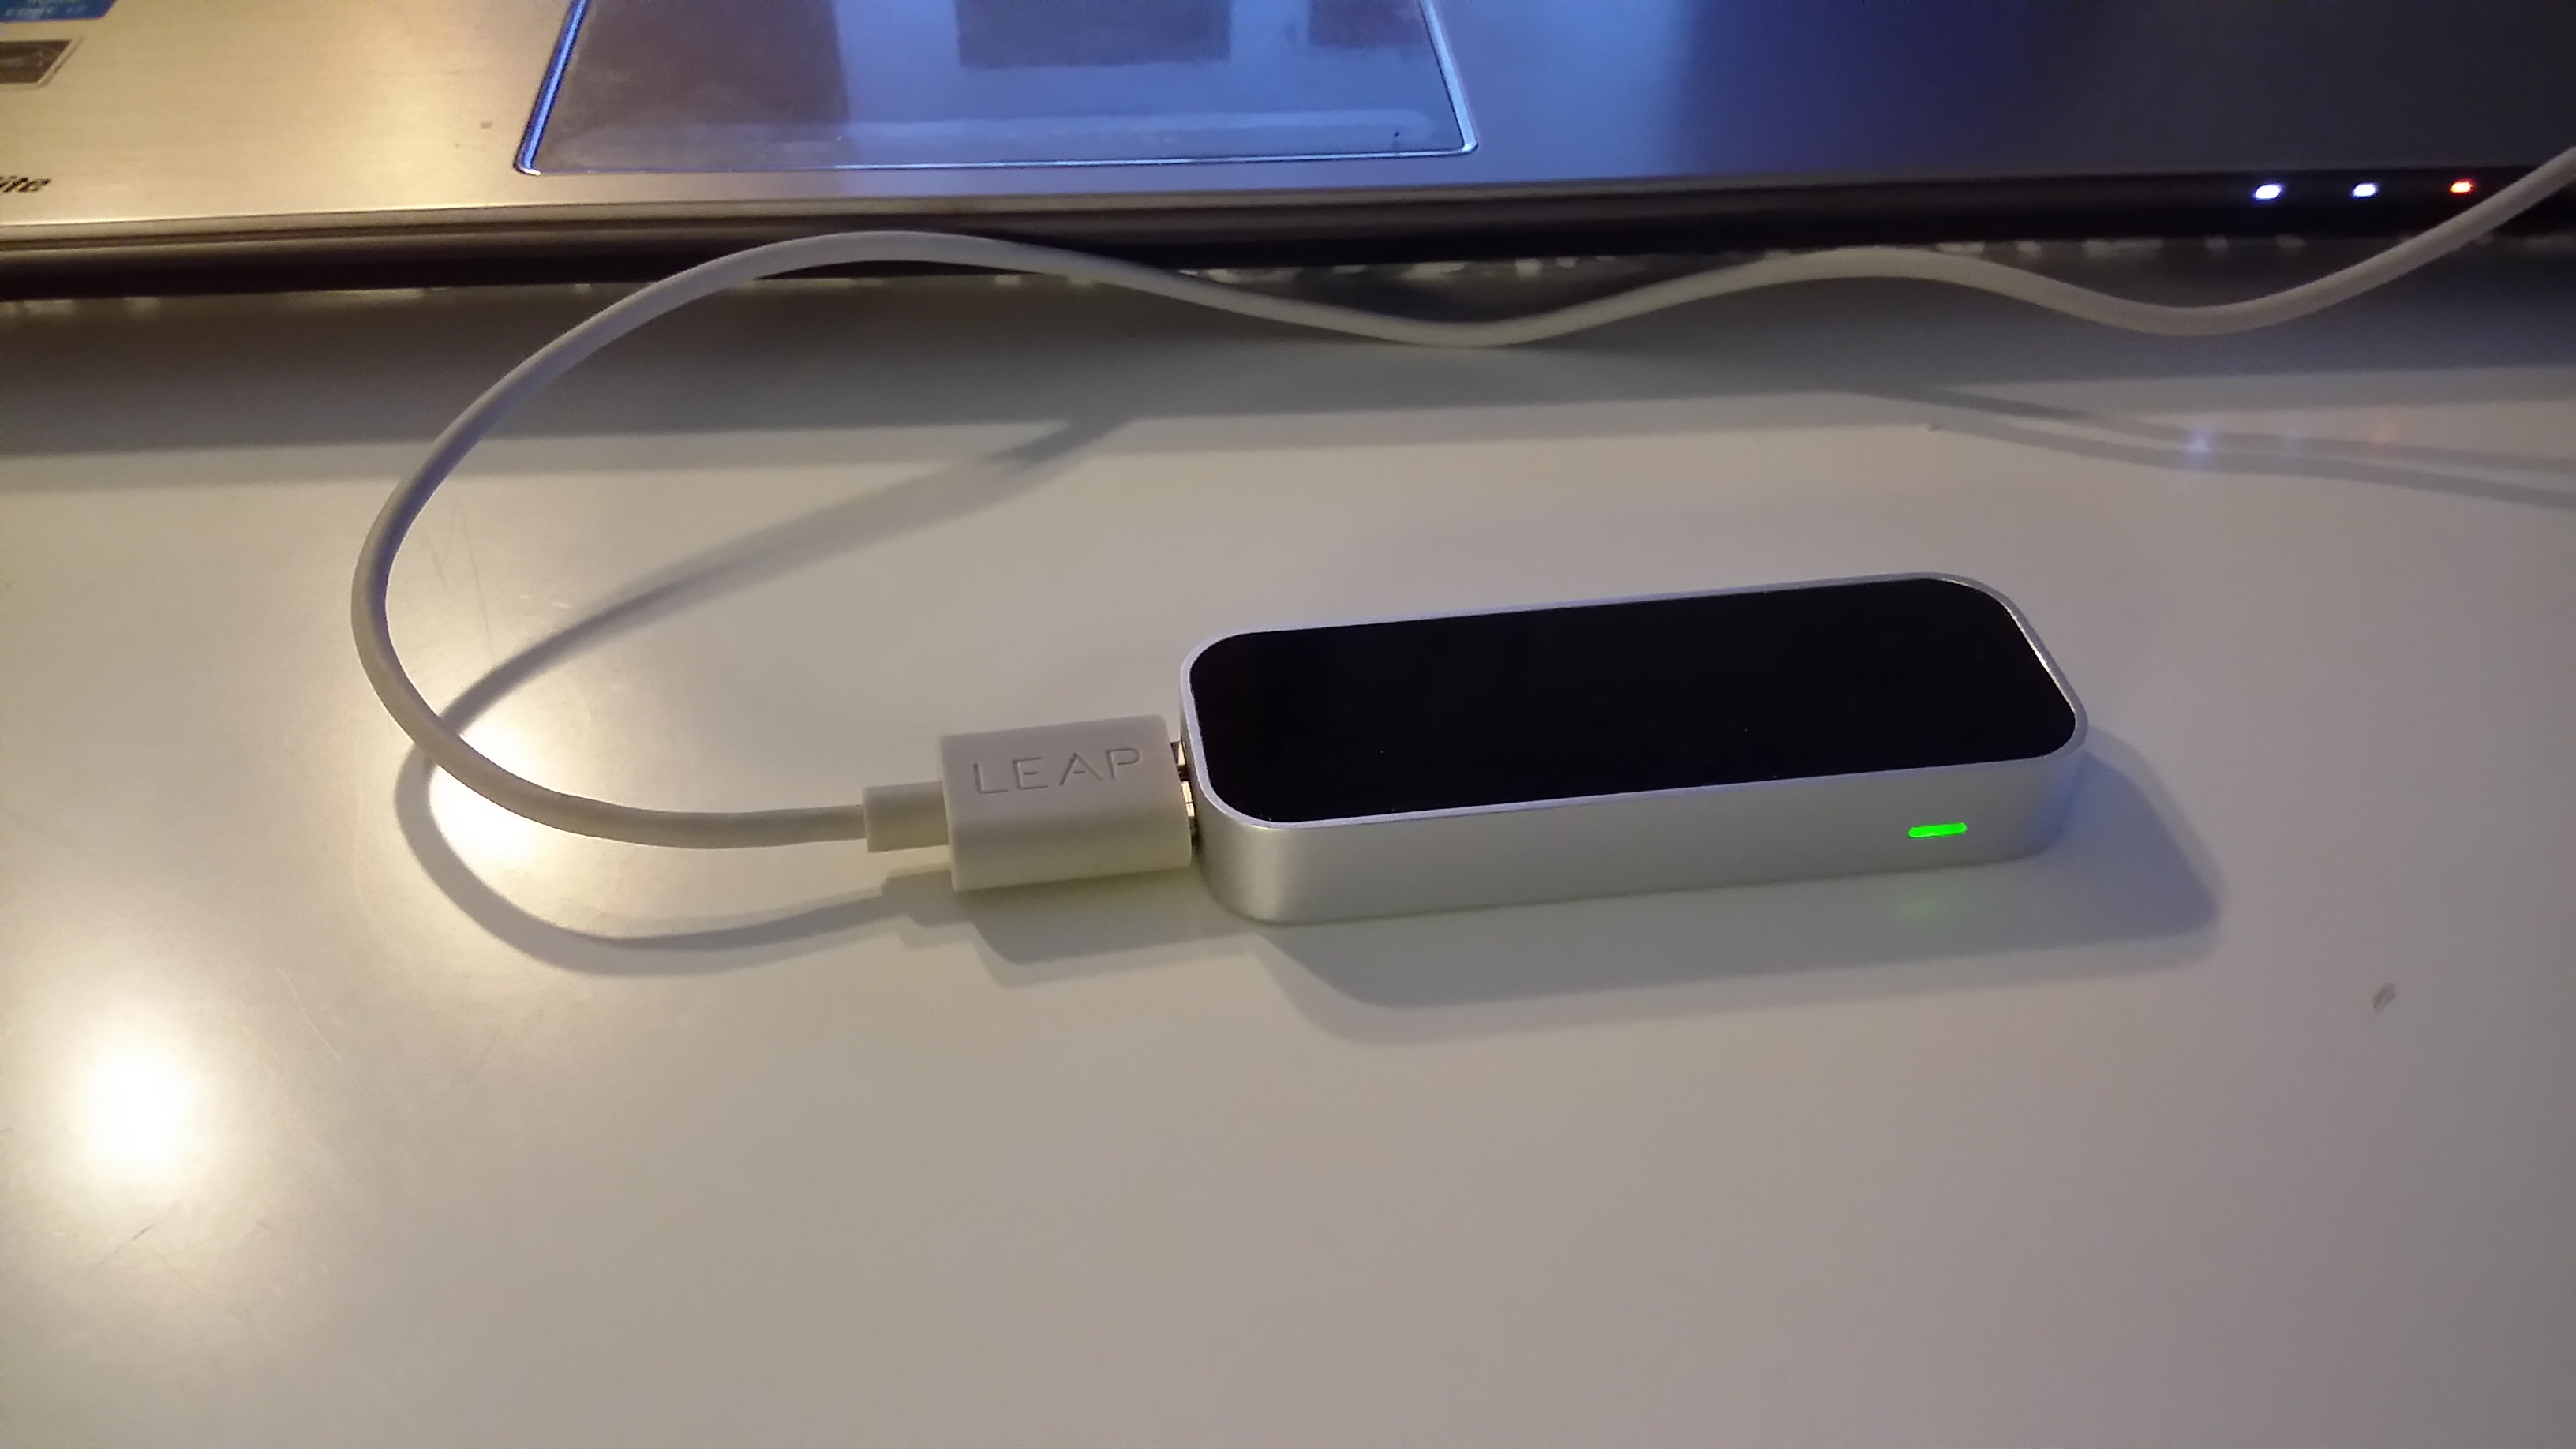
\includegraphics[width=.5\textwidth]{figures/LMdevice.jpg}
  \caption[Leap Motion device.]{Leap Motion device.}
  \label{fig:setup}
\end{figure}

The set up of the equipment needed to be straight forward and fast. An external screen and the Leap Motion device were placed on the table in front of the child. Both, screen and scanner were connected to the laptop. The laptop was place in a way so that the laptop’s screen was not in vision of the test person. All sound that could disturbed during the test session was turned off and the test person could so focus completely on the task.

\begin{figure}[h]  %t top, b bottom, p page | you can also use h to try to get the figure to appear at the current location
  \centering
  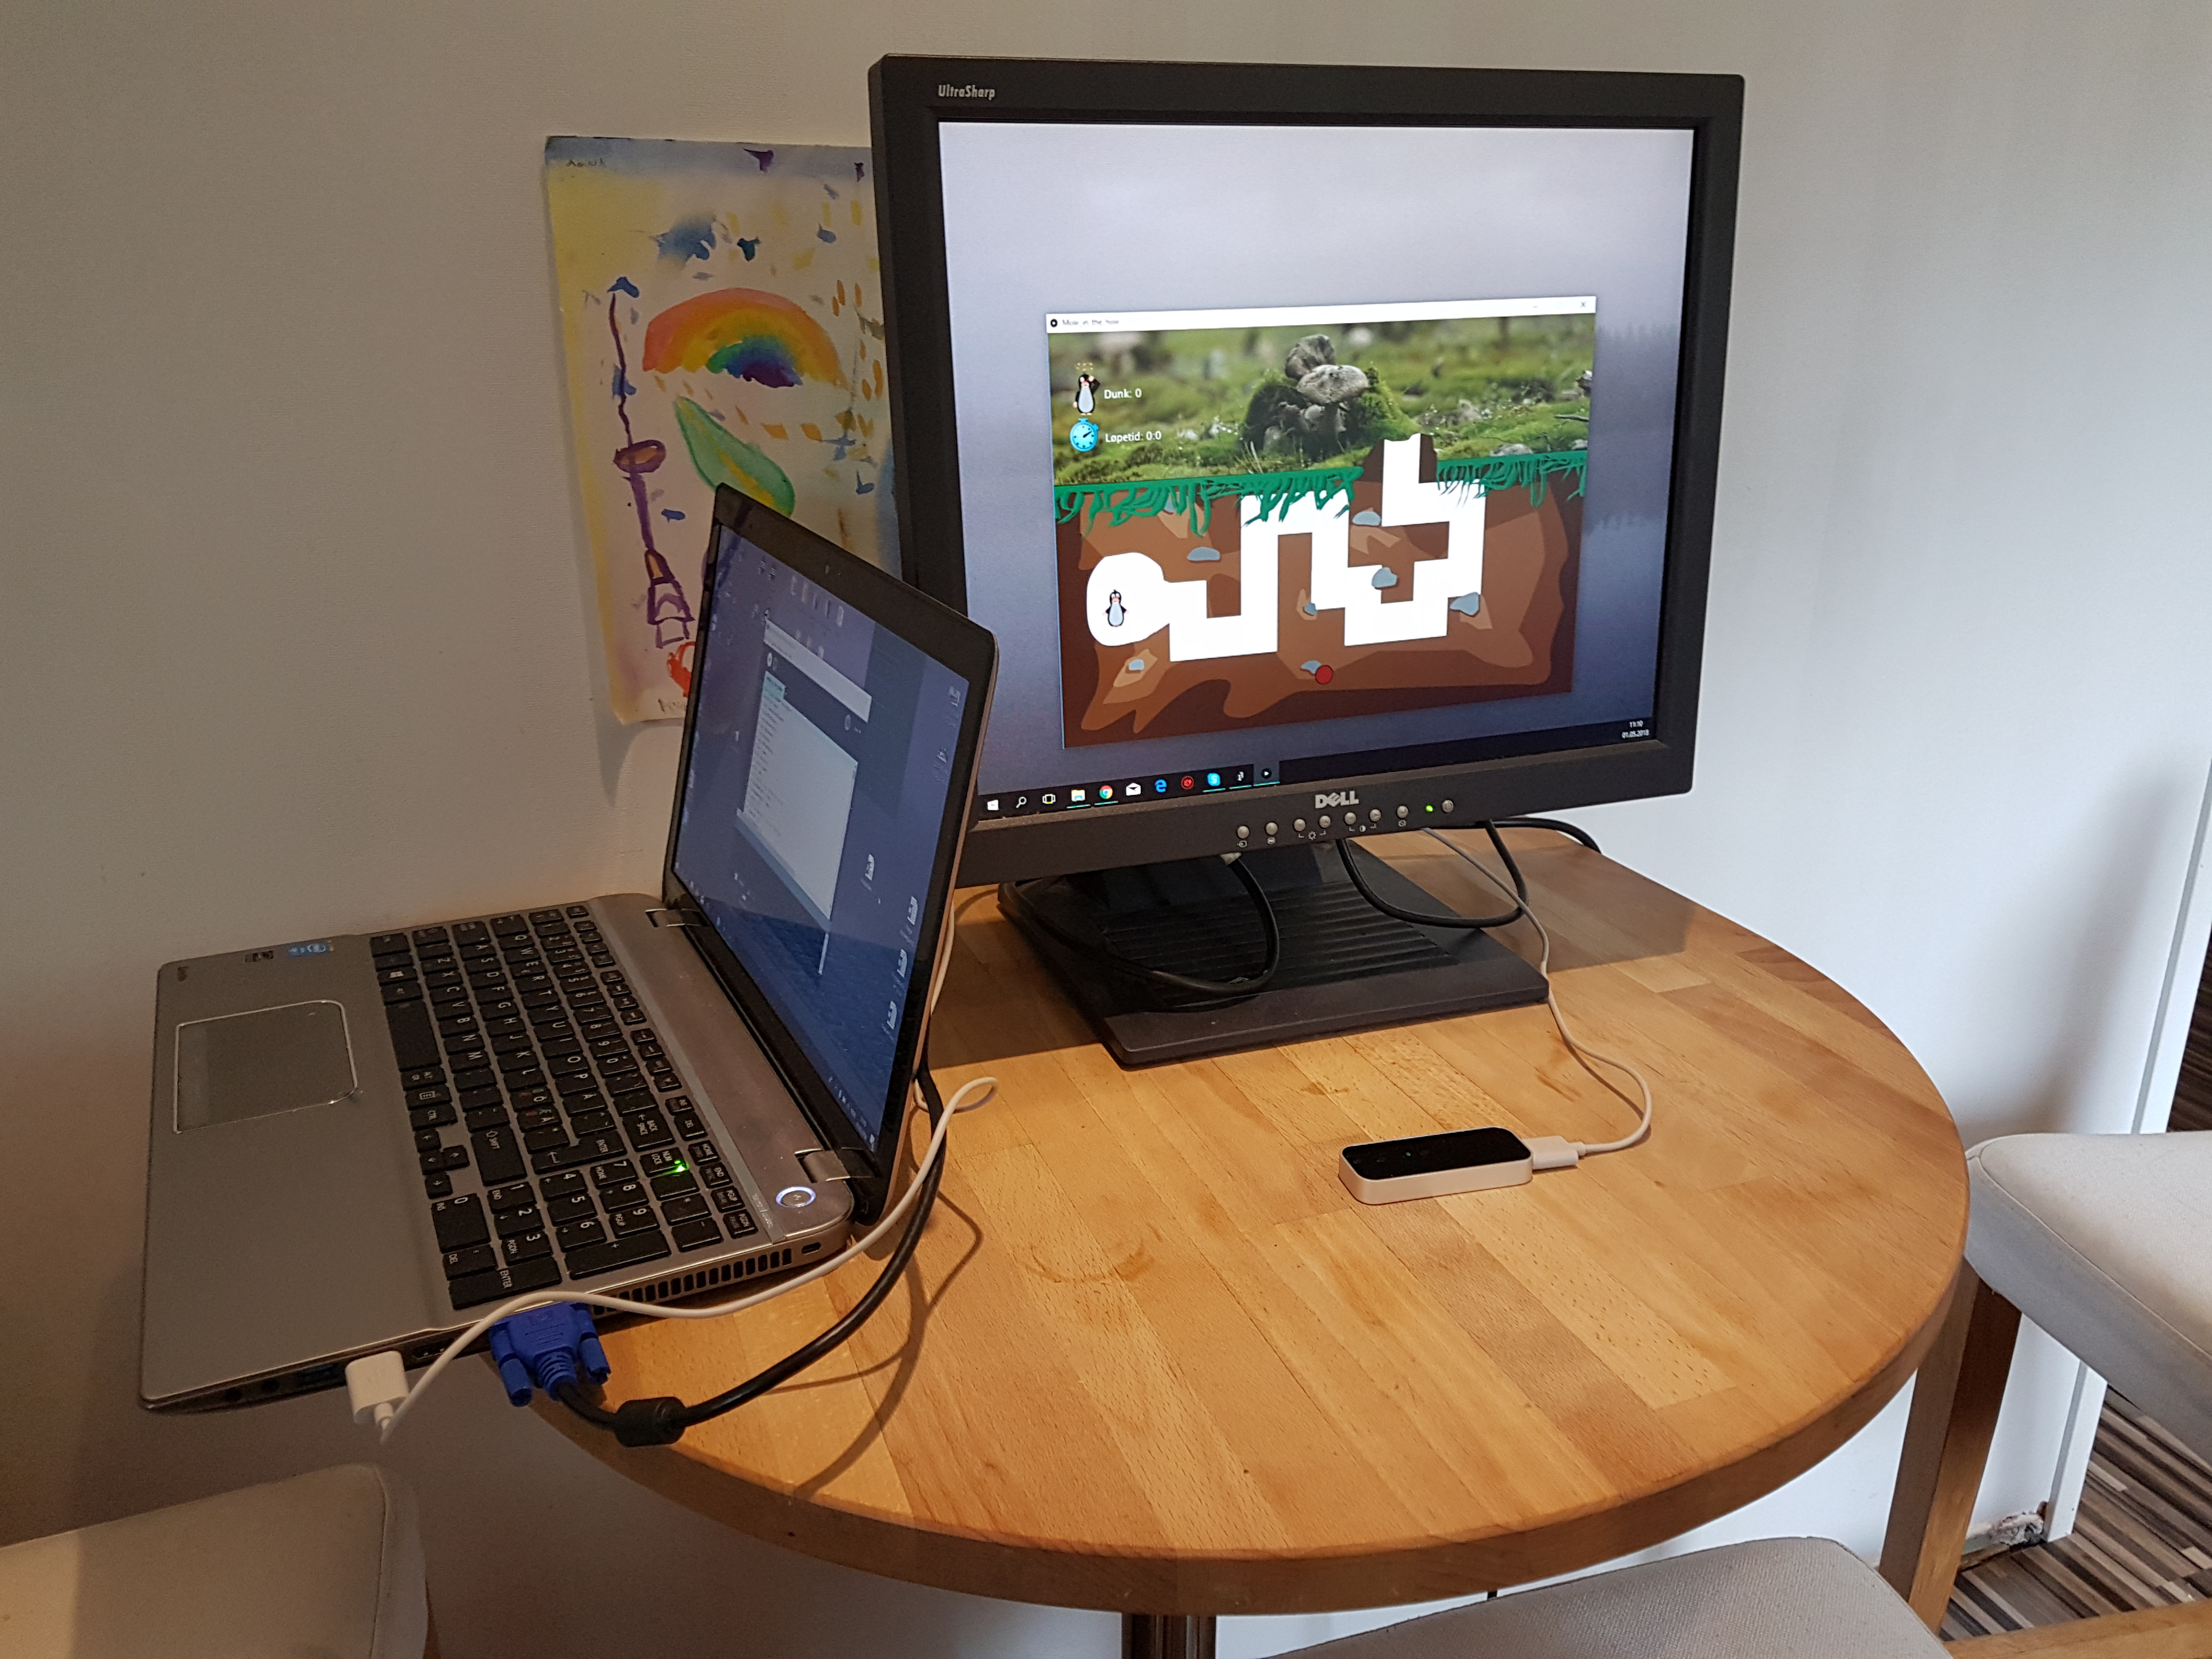
\includegraphics[width=.5\textwidth]{figures/setup.jpg}
  \caption[Equipment setup.]{Equipment setup.}
  \label{fig:setup}
\end{figure}


\subsection{Ethical consideration}
\label{sec:ethical}

Studies involving human participants require considerations of ethical aspects. Children in particularly have to be protected from doubtful research. In this study, ethics, confidentiality and privacy was an important factor during the whole project.
During the experiment, the children were never forced to carry out the task. All involvement was based on voluntary participation. If for any reason a child wasn't cooperative the experiences was canceled immediately. 
It is important to point out that the study didn't collect any personal data. Every participant was registered with a consecutive number which would not reveal the participant identity. The collected data was kept confidential. Only the overall outcome was used for further analysis in order to confirm the hypothesis.  

A concern form was handed to the parents to confirm and sign. The form was downloaded from www.usability.gov and modified for this study. (see attached concern form)


\subsection{Pilot test}

A pilot test was conducted before the real test in order to fine-tune the prototype and test routine and to check if there a other issues to be considered. 
https://www.nngroup.com/articles/pilot-testing/

The person recruited for the pilot test was a young girl in her early teens. She had no pre-experience in hands free gesture applications and was therefore suitable for the task.
The pilot test was conducted some days before the real test.

\begin{figure}[h]  %t top, b bottom, p page | you can also use h to try to get the figure to appear at the current location
  \centering
  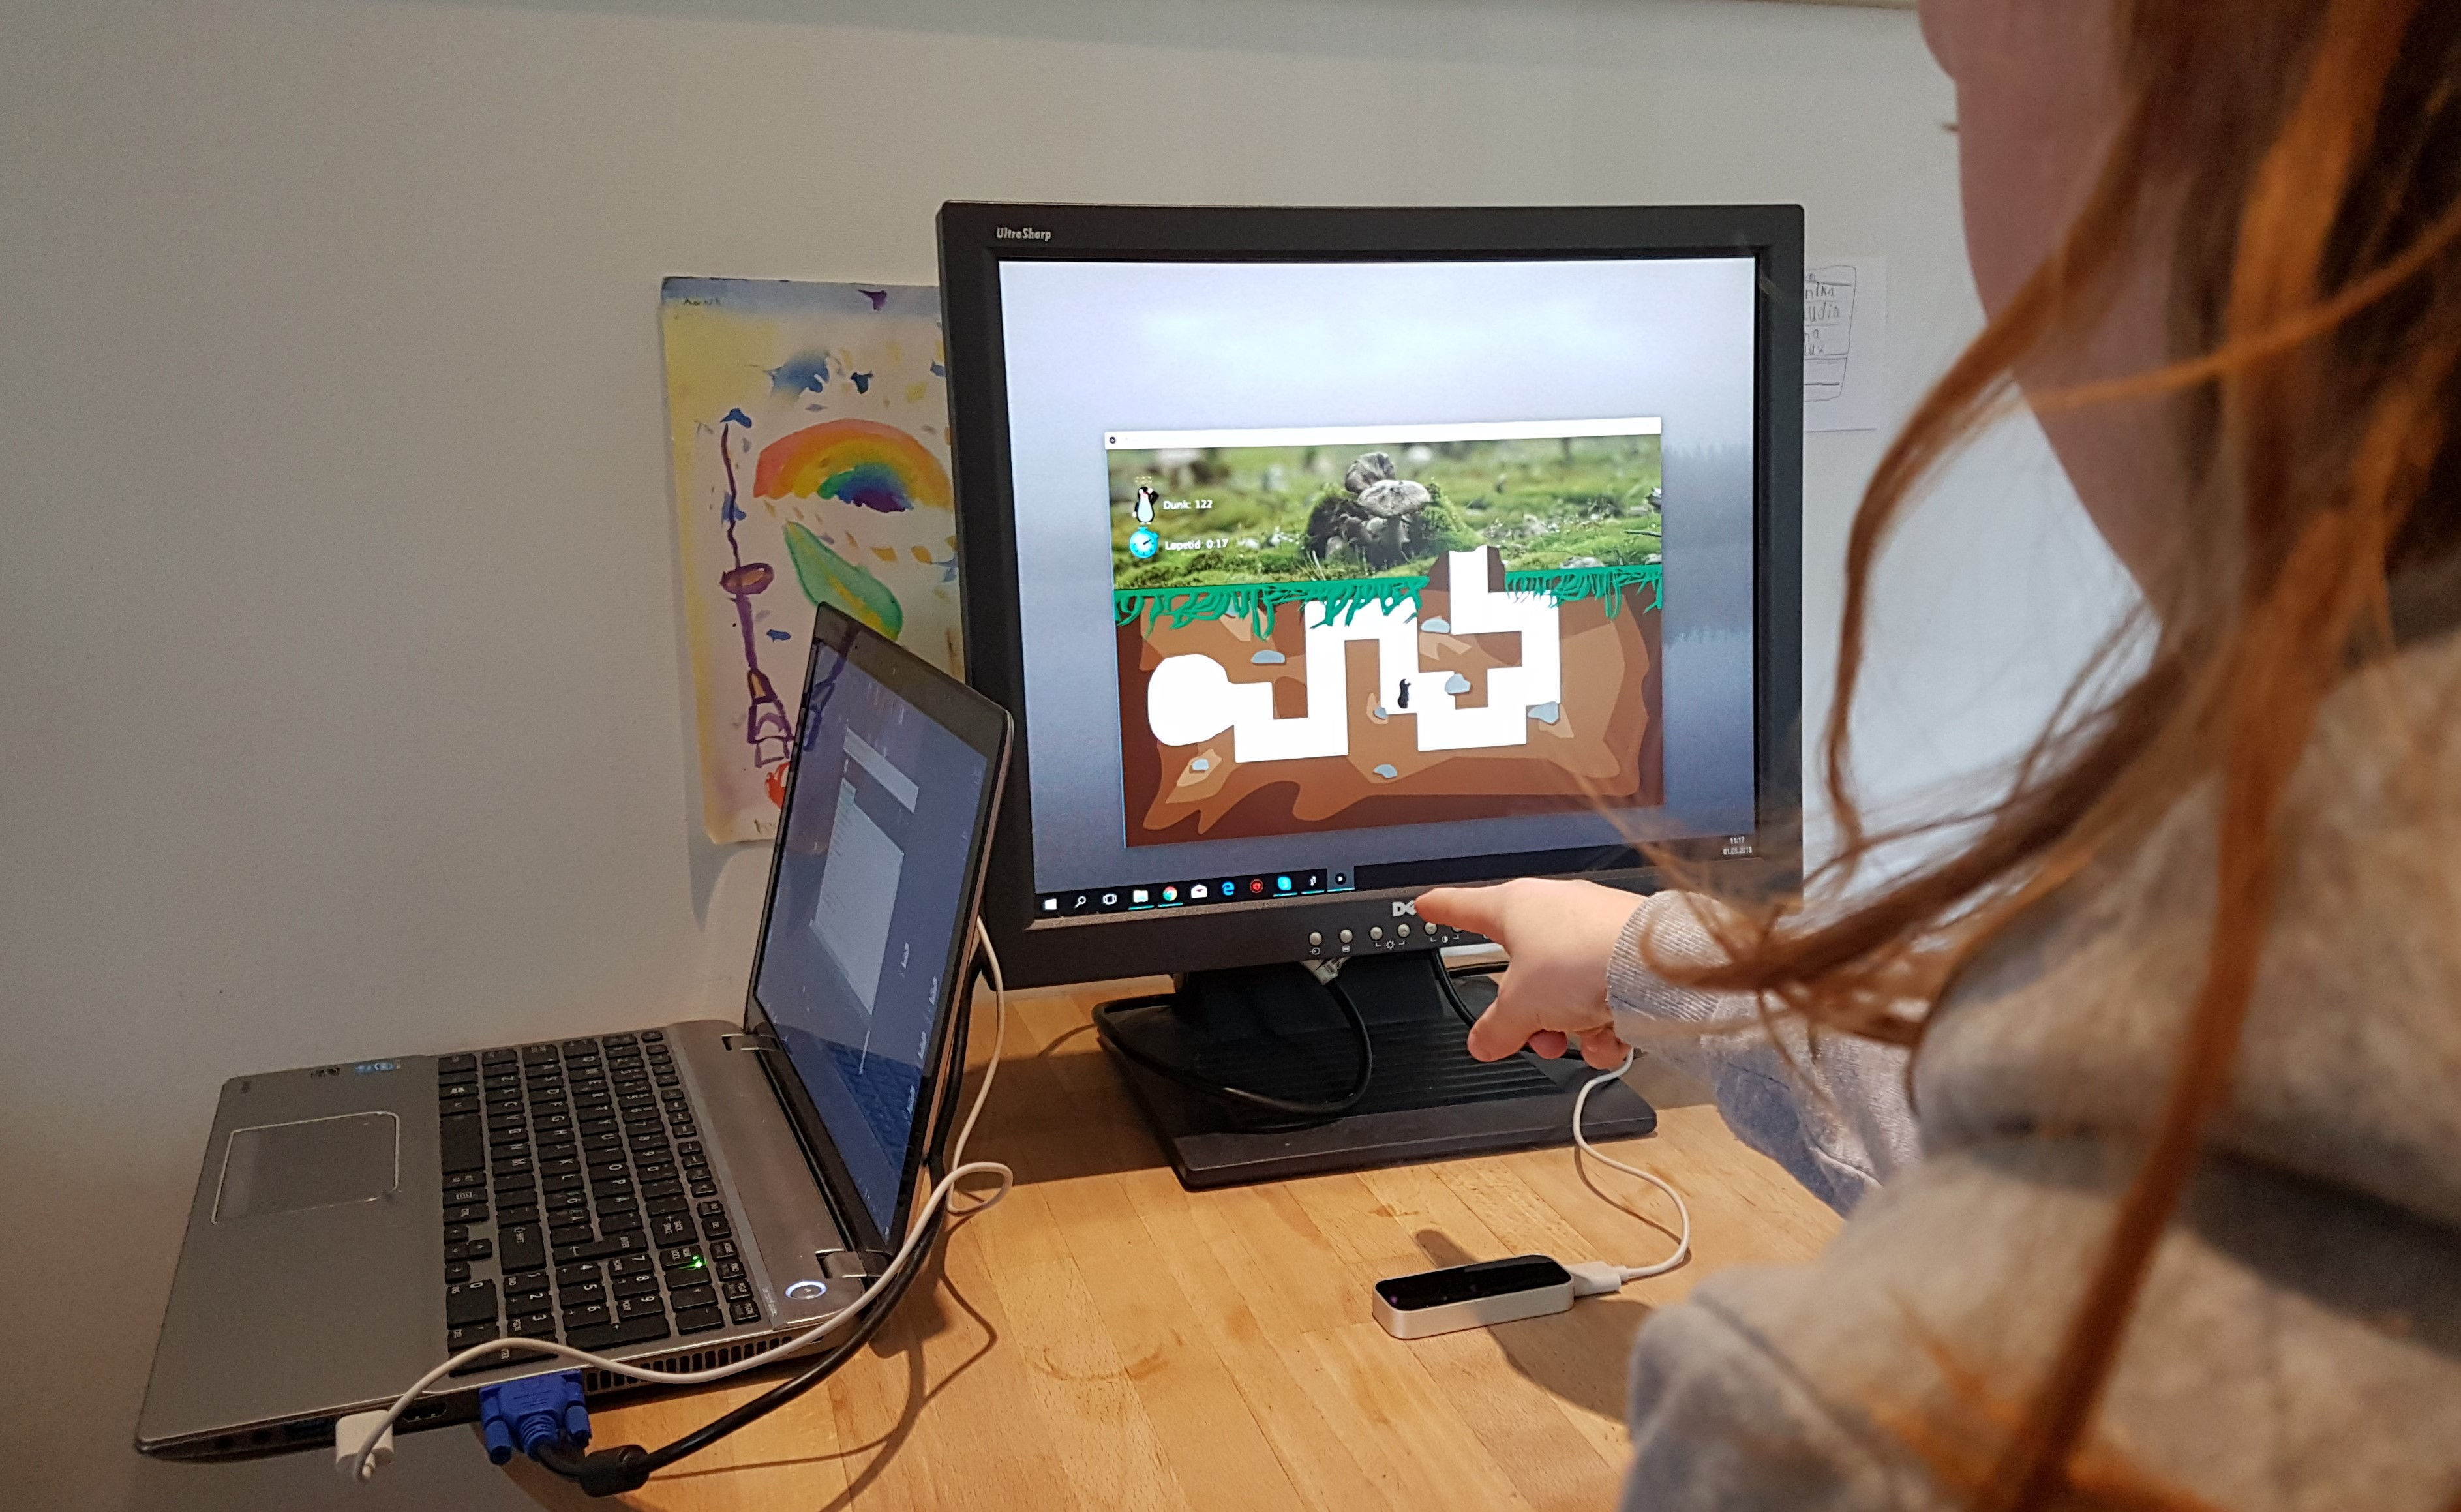
\includegraphics[width=.5\textwidth]{figures/pilottest.jpg}
  \caption[Pilot test.]{Pilot test.}
  \label{fig:setup}
\end{figure}

The pilot test revealed some few issues that needed to be improved or at least to be considered in the real test.  One of the issues concerned the understanding of the system. Since the freehand sensor is a device that still is quite unknown to children,  it is  not enough to say what the participant has to do, but it is  essential to show in advanced how the application works.

The second issue that needed to pay attention is the smiley scale. Since there are different smiley for the scales. Hard-easy and good - bad. It was not a good idea to have them all laid out in front of the participant since this leads to confusion.

The test showed that is was a good idea to have an external screen that only showed the application. 

Furthermore, the test reveal that it is an advantage if the table and the chair have a proper proportion and stands  in relation to the child's body high.

 
The pilot test confirmed the estimated time of 15 minutes of a test run. Additionally 15 min to build up the equipment, have a little conversation with the child, and debriefing.

\subsection{Task description and execution of the usability study}

The purpose behind the usability study was to investigate if the children understand the idea of hand-free interaction. Additionally, the extracted parameters served further analysis. The idea behind that, was to consider a hand-free interaction for medical examination and diagnostic tool. The task of the usability study was about moving the pointer to the mole and than move the mole to the exit as fast as possible while staying on the white path.
The kids also had to perform two gestures in additional, a pointer gesture and a poke gesture. The pointer gesture was needed to navigate and control the game and the poke gesture activated the mole-go-state.

The usability study was planned in advanced on weekends and holidays. Families are usually quite busy and it was quit convenient to organize a meeting on those days.
The equipment was carried and build up at every location on a dinner or kitchen table.

The young participant got explained what kind of technology is used in this usability study, how the Leap motion device works and what the task is.

Considering the still unknown technology, the test moderator showed the participant what the game is about and how to play it. 




\section{Questionnaires}

A short questionnaire was created and used as follow up questions. The questions were about child's own opinion on difficulty, fun, understanding of the game. For the younger participants a smiley scale was create to make the answers more visual and fun and to see if they understand the different facial expression.
The visual scale range from  good - ok to not good and from easy - ok to hard.

\begin{figure}[h]  %t top, b bottom, p page | you can also use h to try to get the figure to appear at the current location
  \centering
  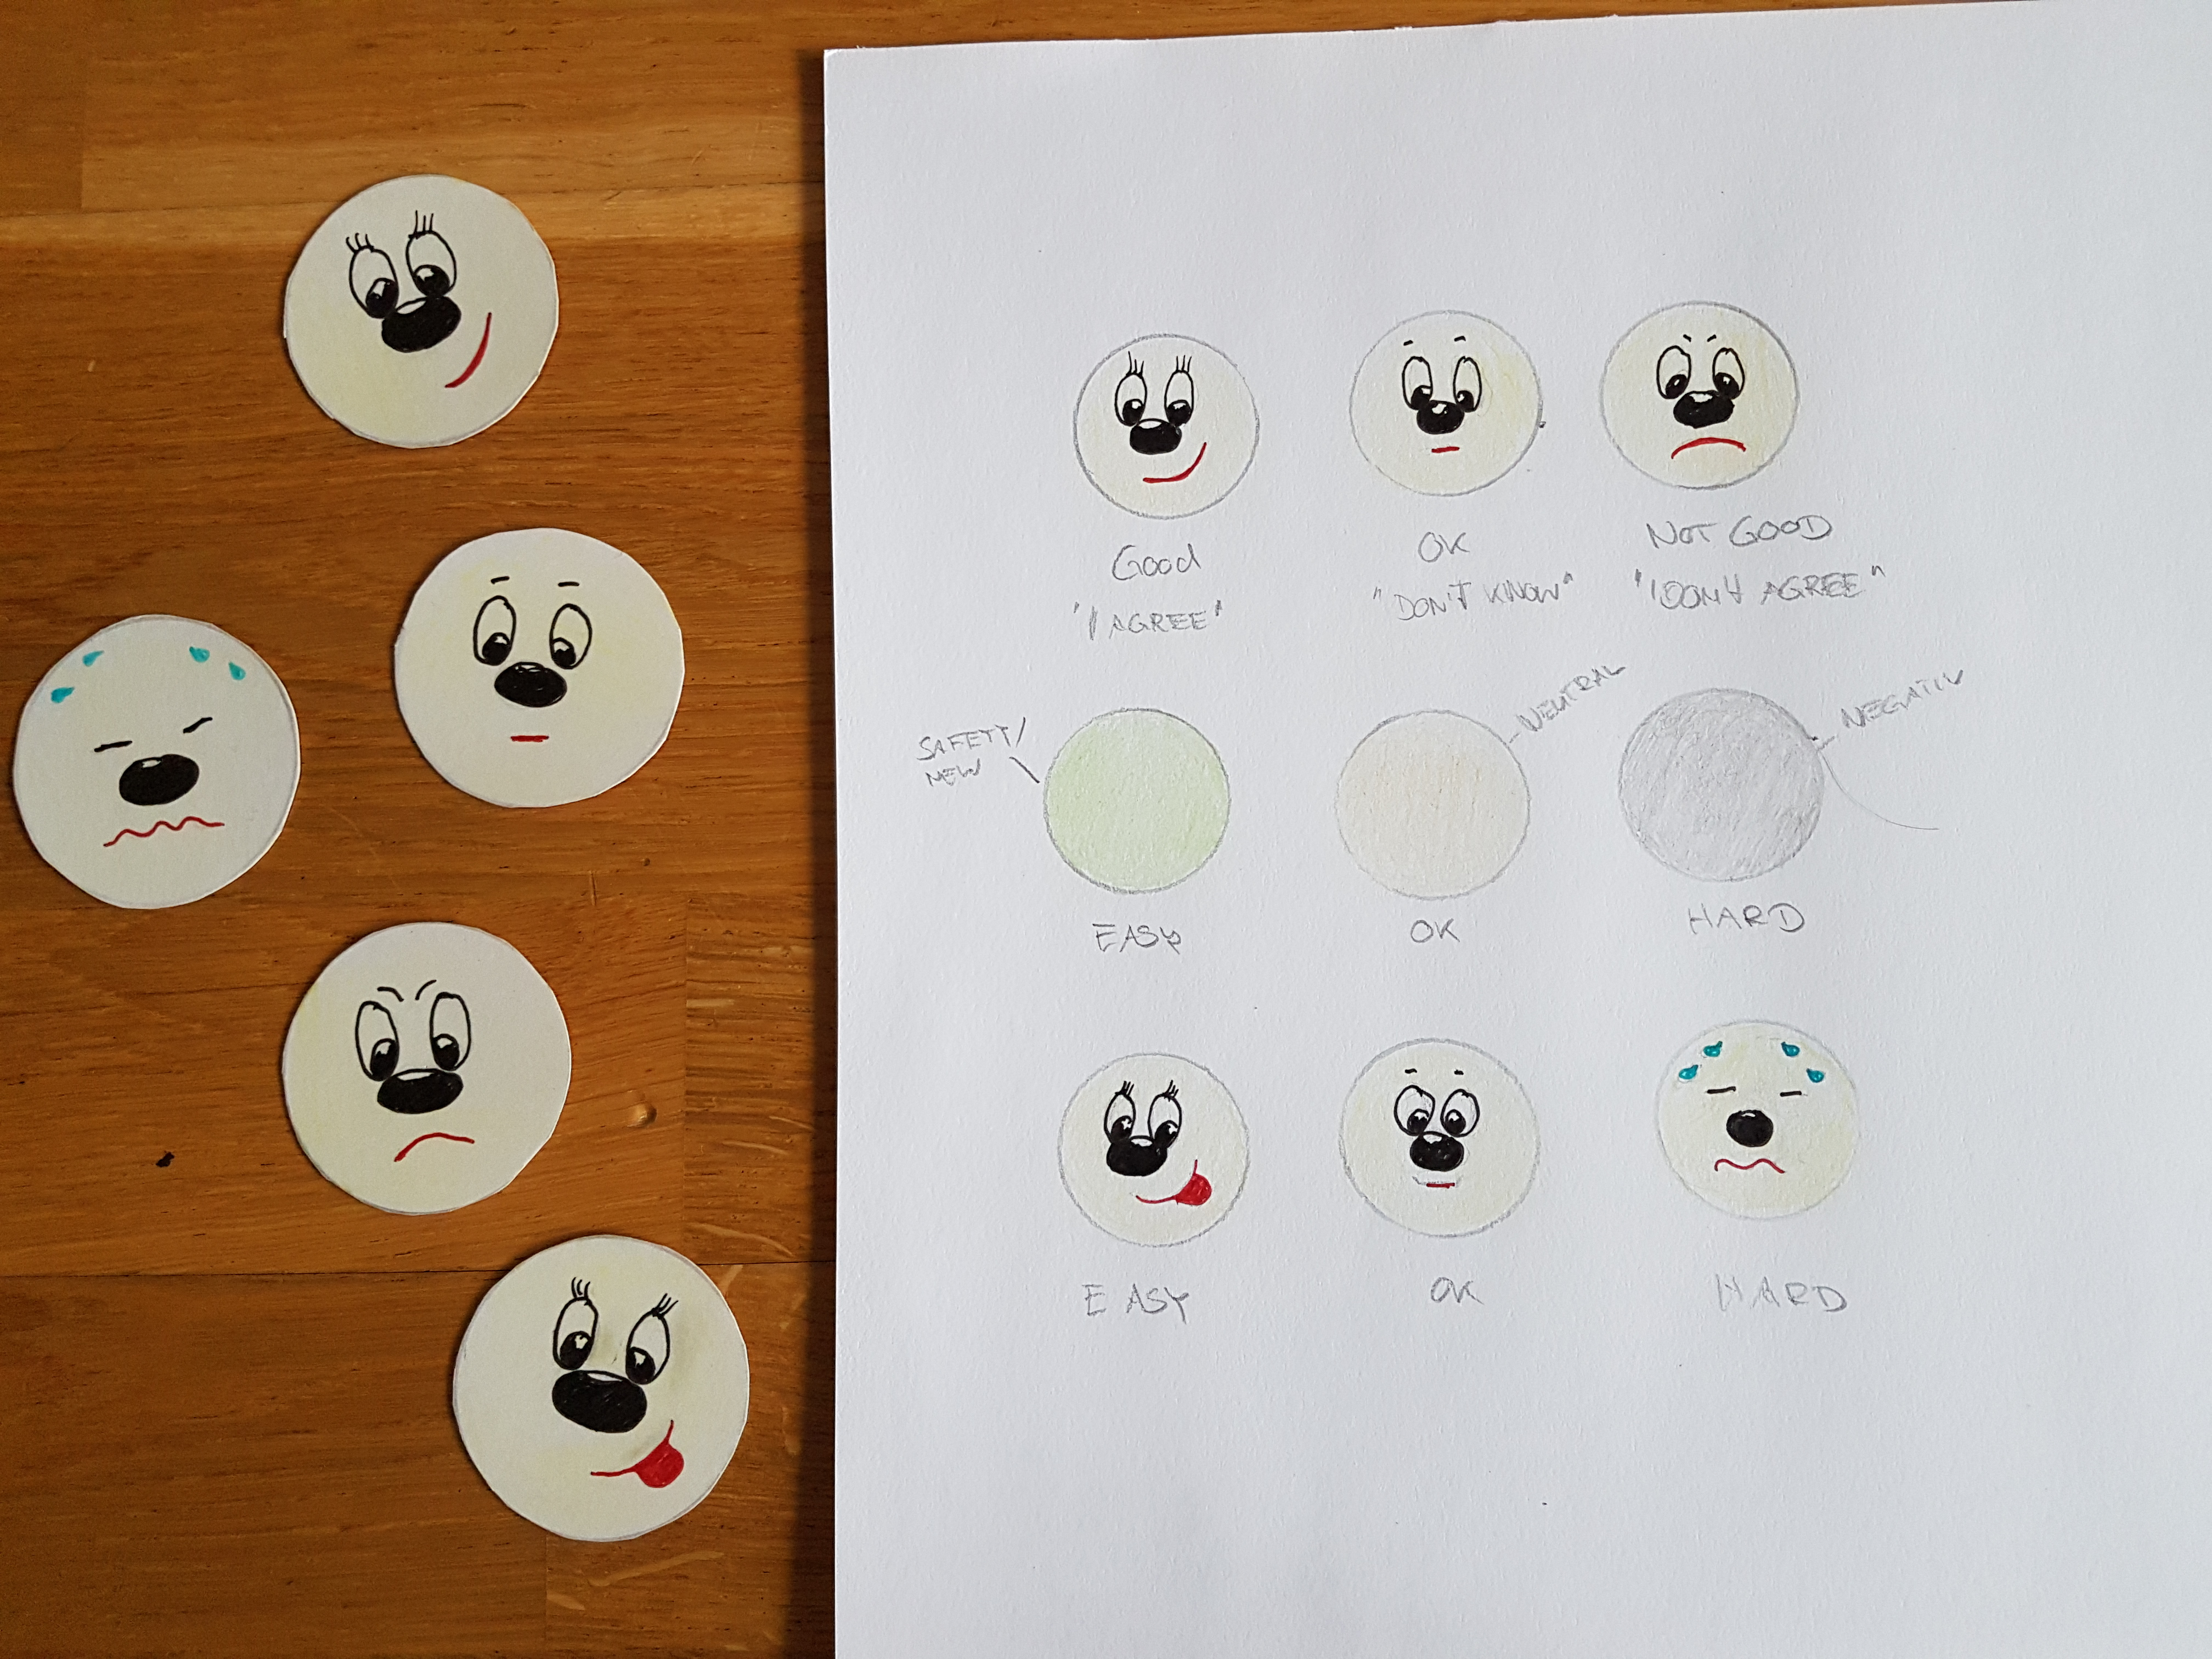
\includegraphics[width=.5\textwidth]{figures/scale.jpg}
  \caption[Visual scale.]{Visual scale.}
  \label{fig:setup}
\end{figure}

The gathered information and data is evaluated and presented in chapter~\ref{chap:dataanalysis} and will be further discussed in chapter~\ref{chap:discussion}.

(see attached questionnaire in the the attachment section.)



\section{Observations}

Observation is a common scientific method and often used in research projects.[reference] 
Observation during this experiment focused on the child's behaviour and reaction during the experiment. Additionally,the ability to perform the task and how much assistance was needed was recorded.
\chapter{Background, theory and existing literature}
\label{chap:background}


\section{Keywords}
\label{sec:keywords}

\section{Gesture definition and guidelines}
\label{sec:gesture}
Gestures are very common in intercommunications between humans. Arm, face and head movements are gestures that are evoked by an idea, emotion or reaction. For a better understanding, gestures accompany verbal information. However in some situations are gestures more suitable than speech, such as in noisy environments (Wagner et al., 2014).
Some HCI researcher classify and categorize gesture in order to differentiate them from each other. McNeill (2005) for instance, categorized gestures into gesticulation, pantomime, emblem, sign language. He then classified gesticulation into iconic, metaphoric, rhythmic, cohesive, and deictic (McNeill, 2005). Pavlovic et al. subdivides gesture into communicative (gestures that have to be learned) and natural hand and arm movements, called manipulative gestures (Pavlovic et al., 1997). Park and Han distinguished between manipulative and communicative gestures, which are a part of a nonverbal component of speech (Park and Han, 2013). Furthermore, an interesting claim made Riener. He pointed out that gestures might differ from gender, ethnicity and cultural background (Riener, 2012).
 
Gesture Guidelines
Gestures can be part of a multimodal application, which can be a solution for people with challenges in everyday life in order to compensate impairments such as speech or hearing disability. Anastasiou (2012) carried out a study where a subject navigated a wheelchair through a set-up of smart home environment by only using speech and gestures. Her study showed that the subjects mostly used gesture when something went wrong (Anastasiou, 2012). Another study, relevant for this project was conduct by van Beurden et al. (2012) which compared gestured-base investigation to device-based interaction  and investigated the pragmatic and hedonic quality of both interactions (Van Beurden et al., 2012). Researchers such as Donald Norman, Jakob Nielsen and Malixia et al. point out the importance of gestural guidelines in order to assure usability and the naturalness of gestural interfaces.(Norman and Nielsen, 2010, Norman, 2010, Malizia and Bellucci, 2012). Additionally, Montero et al. carried out a study on social acceptance of gestural interfaces which describes influencing factors (Montero et al., 2010).



\section{Autistic Spectrum Disorder (ASD)}
\label{sec:asd}

Autism Spectrum Disorder (ASD) is a medical term for a collection of different autistic disorders. (autismus.de ) which includes autistic disorder, asperger disorder and pervasive developmental disorder. These disorders are often practically hard to distinguish and for that reason a medical term ASD was established.  ASD is a complex neurological developmental disorder. The onset of the symptoms are recognized early in the childhood. (NIHM). The development delay and impairment of a child affects the social behaviour, they have difficulties to express semselv and find it hard to communicate with others.Furthermore, children with ASD have often motor abnormal behavior such as repetitive and stereotyped movement (McCleery. lloyd).  ASD is therefore characterized as a social and cognitive disorder.(whyatt) The impairment ranges from mildly to severity and varies from person to person. (NIHM) however, ASD is more common in males than in females (eckert and others). According to autisme.de, studies in Europe, Canada and USA discovered that 6-7 per 1000 people have ASD. 



\subsection{Motor skills associated with ASD}

It is often observed motor delays and difficulties with gross and fine motor coodination ( McCleery) in connection with ASD.  This is also confirmed in serveral studies for instance by Founier et al, Motor delays gets more obvious with age and motor skill fall behind the expected normal chronological age. (lloyd) motor skill are complicated movements that needs coordination and motor planning skills. 
Also imitation problems were found in the research done by  Roger et al
Some researcher refer to motor clumsiness (kanner, Lloyd) as a clinical description of the motor skill disorder.
One of the reason why children with ASD have social, emotional and commicative difficulties is the motor control deficit and eye-hand coordination ineffiency. (crippa). Motor control is important in order to express emotions, social engagement and it corroborates cognitive development. (anzulewixc,) 
Disturbance in motor movements like to gasp, touch, handwriting, bodyposture shift and walk are frequently seen in children with ASD. (azulewicz) Additionally, significant motor coordination and motor timing deficit in individuals suffering from ASD is revealed by several research. (azulwicz)

Research of motor movements in gameplay on a tablets showed that children with autisme used greater force of impact and gesture pressure, a different distribution of force on the devise and faster gestures during the gameplay (anzulewicz). This caracaterixes the motor control deficit on chidlren with ASD. However,  Fast hand movements can be an explanation of eye-hand coordination problems (crippa) Crippa pointed out that the reaction time of ASD patients slowed down  when a higher degree of eye-hand coordination was needed.




\subsection{Diagnosing and screening methods}

Screening is a standardized and systematic process in order to detect early sign of a disability or disease. A screening of young children would ensure that early signs of ASD are detected and diagnosed in an early stage of their live in order to enhance the chance of a better live. (Zwaigenbaum et al. 2015)  
However, it is quite challenging to discover ASD because the diagnosis of autism is complex (Anzulewicz). It relies on specialist and their diagnostic instructuments and how they interpret the data that is gained during the test sessions, observations and interviews with the parents.


In the area of clinical assessment of motor function, test like M-ABC and mullen Scale are used frequently. [Reference]
Lloyd et al used the Mullen Scale of Early Learning ( MSEL) development test for children from 0 to 68 month in his study on motor skills of toddlers with ASD. It is divided into 5 categories,: gross motor, fine motor, visual reception,  receptive language , expressive language.
M-ABC is movement assessment battery where children are divided in 3 age groups. This test focuses on  motor coordination development.  
Other evaluation test for  motor skills may such as  Pearbody Developement and Motor Scale - 2 might be more suitable according to Ozonof et al 2008 (Lioyd))
He also use the Vineland Adaptie Behaviour scale (VABS) which is a standardized parent report. It measures the ability of everydays functioning of the child. Patent Surveys is a cheap method but lacks of precise interpretation.

Systems such as optical motion tracking on the other hand  are an expensive laboratory base system that requires expertise and are more ornate and costly. [Reference]

Anzulewiz et al. pointed out that more accessible and precise computations  system are needed to measure motor performance.


According to nevro.legehandboka.no (http://nevro.legehandboka.no/handboken/sykdommer/alle-sykdommer/alfabetisk-oversikt/autisme-aspergers-syndrom), the Autism Spectrum Quotient (AQ) is a wide used screening tool for initial diagnostic of ASD in Norway. The test consist of a report with 50 questions and a score higher than 32 could indicate Asperger syndrome (AS) .

However, a screening process is often related to time consumption and reimbursement. Zwaigenbaum et al discovered during their literature review that pediatricians complain about insufficient time and compensation and stated this as the biggest hindrance for conducting a screening. Furthermore, other issues concerned the distribution of screenings questionnaires, interrupted work-flow, scoring difficulties and the lack of training regarding instruments for  screening of ASD. In order to gain more acceptance and a regular screening routine, Zwaigenbaum et al, believe that a  screening of multiple disabilities at the same time could be of great interest.



\section{Developmental screening method}
\label{sec:screeningmethod}
Nowadays,checking children for developmental deficit are a part of the routine examination in Germany. In child care centers the children are extensively observed, once a year.
A more detailed examination which is a development screening procedure is carried out at the pediatrician. A so-called "U-Untersuchung" is a non-obligatory examination to detect early signs of development deficit and other diseases.
An additional examination is performed by the educational authority in order to check if the child is ready for school.
In Norway, there are similar routines where childrens are observed and evaluated in relation the the national development plan.

However, this study concerns the procedure of motor skills test methods. A well known method is described in the subsection below. 

%https://www.familie-und-tipps.de/Gesundheit/Kinderkrankheiten/U-Untersuchungen/

%https://www.kindergesundheit-info.de/themen/entwicklung/frueherkennung-u1-u9-und-j1/


\subsection{The Movement Assessment Battery}
There are several clinical instruments for testing children on motor performance and other capabilities. The Movement Assessment Battery - second edition (M-ABC2) is a well known test battery for motor-coordination capability of children from 3 to 16 years of age. It provides a standard performing test and checklist and is designed to identify motor coordination impairments. However, like other test methods, M-ABC2 has its considerable strength and weakness. For instance, Ted Brown [reference] pointed out the lack of reliability and validity of this test.

Dr. phil. Thorsten Macha provides a useful overview of several test methods and procedures including M-ABC2. He describes specific motor exercises to test manual dexterity, ball skills and balance. 

Exercises suggested for the M-ABC2 test were the point of departure for this project and the possibility of digital implementation was explored.



%http://entwicklungsdiagnostik.de/motoriktests.html


%https://www.tandfonline.com/doi/abs/10.1080/01942630802574908?src=recsys&journalCode=ipop20

\section{Leap Motion}
\label{sec:leapmotion}
\section{Serious games}
\label{sec:seriousgames}
This project is about the assessment of a hands free device and gesture-based computer games as a medical evaluation tool. A medical evaluation tool in form of a computer game is referred to as serious games. Serious games are computer games that are not for entertainment and pleasure but they are specialized for a more serious purpose. 

The concept of serious game startet in the early 1970’s. Abt (reference) stated that “...these games have an explicit and carefully thought-out educational purpose and are not intended to be played primarily for amusement.”
Considered as the  world’s first serious video game was launched in the USA in 1972. The game that was a potential educational tool was called Odyssey. Other educational games like “The Oregon Trail” and “Lemonade Stand followed soon after. (Fedwa)
The first simulation tool was launch for the American armee in 1981.  The game called “The Bradley Trainer” was developed for training purpose of the Bradly tank.
The market for serious games is a remarkable business and has a enormous growth rate in the lately years. That means that a lot of effort is put into this area and the demand of such systems is significant.(Fedwa)
An interesting classification of serious games was suggested by Ratan et al (Refernce). They classify serious games in four section: [1] educational for academic and social change and health, [2] practicing skills and problem solving, [3] target age group and [4] game platform.
Laamarti et al (2014) also made an attempt to classify serious games. They started with to define the characteristics of serious game that includes activity, modality, interaction style, environment and application area. 

There is a tremendous development of serious games in different areas. Laamarti et al (2014) named domains such as training, education, health care, well-being, advertisement, cultural heritage,  interpersonal communication and others. 
For this project, the area of  biomedical and health care is of interest and will be explored further. The aim of  serious games in health care is to provide knowledge and skills within the medical domain in order to simulate situations, to guarantee safety, to lower the budget and much more. According to Laamarti et al (2014),  serious games for health care can be classified into health monitoring, detection and treatment, therapeutic education, prevention, and rehabilitation. Due to the fact that a neurological disorder affects many millions of people,  rehabilitation of motor skills can have a significant influence on the development of serious games. For recovering from brain lesions a game named The rehabilitation Gaming System (RGS) was designed which can be use either at home or in clinic. Finger, wrist and elbow  movements are recorded with a help of data gloves and video camera.  [Reference: Cmeirao]

Concerning factors that makes a serious game successful, the literature showed that researcher point out factors for serious games that motivates, stimulates and pleases the player. [Reference Laamarti]To name just a view, these factors are background music for motivating players, providing guidance to prevent confusion, avoiding negativity, visibility of displays, multiplayer collaboration, providing syllabus for educational purpose, provide an appropriate challenge for each level.
Laamarti el al (2014), tok those factors in consideration when they proposed guidelines regarding the design and development of serious games. They suggested that row of design elements such as software should be user-centered, multimodal, invigorate virtual connectedness, the possibility to adapt to players, standard evaluation i order to gain higher credibility and sensory- based stimulation.
Interestingly, they pointed out the need of focusing more on natural interfaces in serious game design. Additionally, the success of a  serious games is characterized by terms like  pleasurable and engaging although the game has a serious goal. However, a good balance between pleasure and purpose is essential when designing serious games.
Other important elements that needs to be taken in consideration when dealing with design of serious games are fantasy, fidelity, and context. (Charsky (2010)).  These three elements are of great value because they provide authenticity, assist in recognizing and understanding demanding context.
Tong et al (2016) did a research on serious game based screening tool in order to see if it is possible to use such games as a tool of prediction for delirium. They believe that serious games are promising for cognitive screening in clinical settings.  Based on their research they recommend multiple gesture to maximize interaction, incorporate validate psychological task , the game should be joyable and easy, there should be multiple version of the game in order to adjust the needs of diverse target group. 
Another research on serious game as screening method  was made by Boletsis et al. They developed Smartkuber, a serious game for cognitive screening of elderly players. The interaction tool for this game was based on Augmented Reality (AR). They pointed out the disadvantage such as psychological stress related bias, improved performance through the learning effect, lack of motivation and economic burden, of nowadays standard pen-paper and computational test. On the other hand, the advantage of cognitive screening serious games as a screening tool can be significant as they save time and cost, are more accurate, reduce psychological stress, are joyable and self-administered, just to name a few.  Though the gameful interaction and stimulating exercise the players cognitive ability was screened and monitored on a frequent basis. The obtained result was more objective since the game was played on the players premise, this means the players decided time and place of their choice. They minimized the learning effect through randomized minigames. 
 


The literature review showed that there is a few research on serious games in the area of medical research and screening. (Tong, Ben-Sadoun) Unfortunately, the literature review provided very little relevant information within ASD and gesture hand free serious games which could be useful for this study.



\section{Design principles for gesture interfaces and design criteria for SG}
\label{sec:designprinciples}
Donald Norman created design principles as a guide when designing everyday things. He stated that that a conceptual model is important to manage everyday thing, because humans need to foresee the consequence of their behaviour. Otherwise, people do things by habitual repetition and get in trouble if something goes wrong because they do not know how things are interrelated (Norman, 2002). Another issue that Norman pointed out is visibility. The danger with invisible function is that user can forget them, the system gets less understandable and the operations become more difficult. Norman also mentioned the principle of feedback, an essential point for science of control and information theory. Feedback is about notifying the user who just has performed an action. Ideally, if a human is able to mentally perceive the meaning and understands how to interact with a system, then the principal of affordance is achieved. The lack of these principles is something that Nielsen pointed out when he tested the Kinects gestural interfaces in 2010 (Nielsen, 2010).  To make gestural interaction with touchless interfaces user friendly is important for it success in the future. The question is if Normans design principles are outdated or still valid for gestural interface and can these be the point of departure for touchless interface design or must are new principles needed.
Gestural touchless interface is a great idea. However, when creating such interfaces it is important to understand the challenges it arises. Gestural touchless interface must be designed universal and provide the user with good user experience. It is essential that every user understands the system and knows how to control it. Otherwise, the user gets frustrated and discards the system. For that reason, it is important to investigate what effect the gestural interfaces have on the use, how user responds to gestured controlled interfaces. The outcome then points out difficulties and challenges which is of great value for designers and technologist.

Design criterias for serious games


\subsection{ISO standard}
\label{sec:isostandard}



\chapter{Aims and objectives}
\label{chap:aim}
%Aims describe what you want to achieve. Objectives describe how you are going to achieve those aims.

Poor motor performance skills can be an indicator for various development delays such as Autism Spectrum Disorder (ASD).
ASD is a disorder that has been increased in the population in the last years. The main reason for that is that methods for discover ASD has been improved and knowledge about the disorder has expand and child care personnel has been educate to look for symptoms in early stage of the child's development  \cite{Folkehelseinstituttet2015}. %(https://www.fhi.no/fp/barn-og-unge/utviklingsforstyrrelser/autisme---faktaark/)
Various research has been done to highlight methods (reference) discovering ASD and to emphasize ASD therapy possibilities. Nowadays, standard evaluation tests for instance, M-ABC2, MOT4-5, BOT2 are used by psychologist in order to determine development delays \cite{Macha2010}.
Tests such as M-ABC2, evaluate children's motor-coordination skills. Their test methods focus on evaluating of hand dexterity, balance and ball skills. Furthermore, research showed that children with ASD have disruption of normal movement pattern which also is an indication of motor coordination deficit.(reference). However, according to (reference), test methods that could determine ASD are expensive, time consuming and demand a laboratory environment. A Laboratory is an artificial environment where indeed influencing factors can be controlled but on the other hand such environments can also affect children's behavior. Some become uncomfortable and insecure which in worst case, distort the result. (find REFERENCE) For that reason, the aim of this project is to investigate whether mobile sensors such as Leap Motion and gesture interaction could be used as a supplementary evaluation and screening tool for motor development delays. Furthermore, the research will show if this is a convenient measurement tool to determine ASD in an early stage. The benefits of using Leap Motion are many, as for instance the portability and low acquisition cost. The evaluation can happen anywhere, even in an environment where kids feel comfortable and familiar. Leap Motion is a sensor for gesture controlled interfaces. Nowadays, evaluation exercises are more or less analogical, according to the aforementioned interviews and as described by Macha \cite{Macha2010}. %(http://entwicklungsdiagnostik.de/m-abc-2.html) 
However, a digital evaluation tool could be more appealing to the contemporary technological standard. Since Leap motion is able to screen fine-motor movements, it would be a suitable evaluation tool which is enjoyable, accessible and economical.

%sløyfe denne setningen?
Moreover, the Leap motion sensor may not only be a usefully screening tool but it might be used as a therapy tool for fine motor exercises as well.

%objects -  how to achieve aims
%create a system
%do an experiment

In order to achieve the aim of this project a concept needed to be created and tested. This concept had to fulfill the requirements of the Leap Motion sensor and gesture interaction and also address various parameters. As mentioned in section \ref{sec:asd}, ASD is defined by several deficits such as motor-coordination deficit, sensory-motor deficit, motor-timing disruption, psycho-motor deficit, etc. These parameters are en essential brick for this concept.

A software game is a convenient approach to combine sensor and gesture interaction. This concept would have several modules in order to satisfy various parameters. About 5 modules or less would be enough to checks the capacity of motor coordination and hand dexterity. An example of modules which could be suitable for this concept is described below:  

\vspace{5mm} %5mm vertical space
\hfill \break
Module 1 - Ladybug\newline
Task description: The goal of this task is to put as many ladybugs on a three a possible in a certain time frame. The child has to move a ladybug from the ground up to the tree by only his/her index finger.
Evaluation parameters: count the amount of bug are move in a given time period
Based on: M-ABC2 ( insert coins task)
\vspace{5mm} %5mm vertical space
\hfill \break
Module 2 - Flying balloon\newline
Task description: Flying balloon is a pointing game where the participant must hit the balloons in order to burst them. The balloons are moving over the screen entirely arbitrary. The goal is to burst as many balloon as possible in a certain time period.
Evaluation parameters: Hand eye coordination, accuracy and timing
Based on: M-ABC2 
\vspace{5mm} %5mm vertical space
\hfill \break
Module 3 - Mole in the hole\newline
Task description: The goal of this game is to guide the mole out of his hole. This is a precision game which demands concentration and patience 
Evaluation parameters:  precision, concentration, patience 
Based on: M-ABC2 for hand dexterity test - trace a track
\vspace{5mm} %5mm vertical space
\hfill \break
Module 4 - MEMO \newline
Task description: The game builds on the participants memory ability.  The participant will see a row of objects and the corresponding gestures for a certain amount of time. The participant has to memorize the gesture belonging to the object. Than the object appears on the screen and the participant has to remember the appropriate gesture. 
Evaluation parameters: remember and recall. This is a cognitive task for testing of psychomotor deficit.
Based on:
\vspace{5mm} %5mm vertical space
\hfill \break
Module 5 - Freehand drawing\newline
Task description: In this game the participant is asked to draw a shape with a the pointing finger.  The participant will see a shape on the screen and needs to repeat the drawing. The participant could also be ask to make an existing shape smaller or bigger by pinch movements.
Evaluation parameters: fine motor coordination
Based on standard tool: DMB (trace geometrical forms) and LOS ( paint circles in the air)

%\vspace{5mm} %5mm vertical space
%\hfill \break
%To sum up autism is defined by:
%\begin{itemize}
 %   \item Motor-coordination deficit
  %  \item Sensory deficit
  %  \item Motor-timing disruption
  %  \item Psycho-motor deficit
  %  \item Disruption of normal movement pattern
%\end{itemize}


%\begin{center}
%\begin{tabular}{|c|c|c|c|c| }%| m{1cm}| m{1cm} |  m{1cm} | %m{1cm} | m{1cm}|} 
% \hline
% Parameters - identify ASD & Task description & Deficit/
%Disruption & LM parameters &  Game/task \\ 
% \hline
% \hline
% cell7 & cell8 & cell9 & cell8 & cell9 \\ 
% \hline
%\end{tabular}
%\end{center}

\begin{figure}[!ht]  %t top, b bottom, p page | you can also use h to try to get the figure to appear at the current location
  
  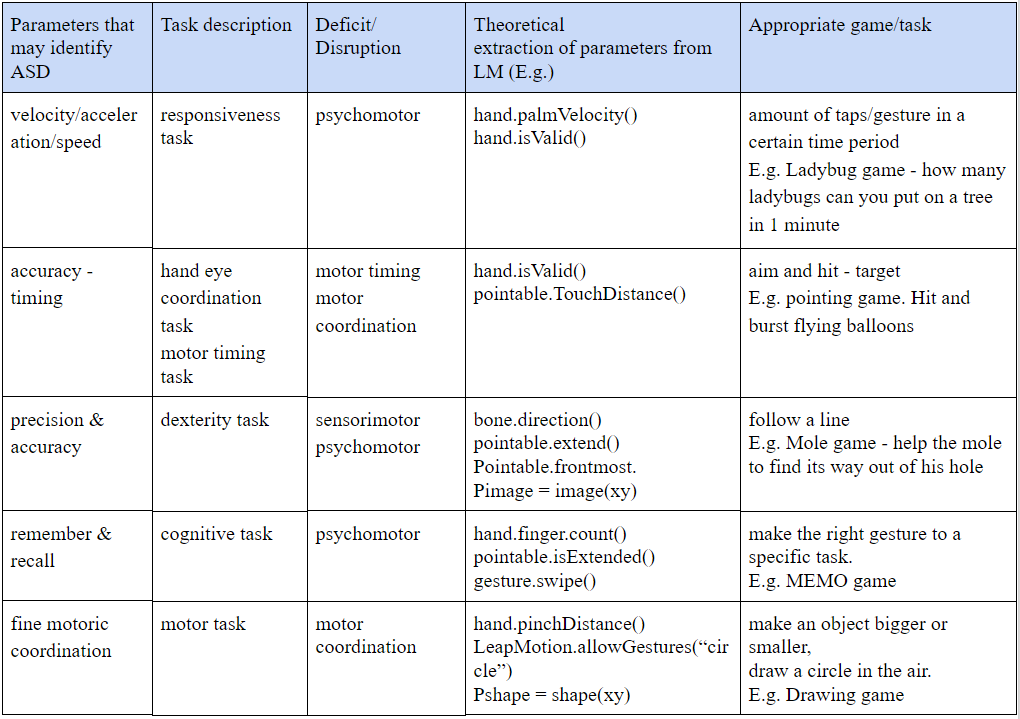
\includegraphics[width=1\textwidth]{figures/tableOfModules.png}
  \caption[Parameters and Modules.]{Parameters and Modules.}
  \label{fig:tableOfModules}
\end{figure}

\vspace{50mm} %5mm vertical space
\hfill 
\break
\section{Research Question and hypothesis}
\label{sec:researchquestion}
Defining the research question and formulating the associated hypothesis is the point of departure for all kind of research in order to find an answer of a specific problem.
\newline
The purpose of this project is to investigate if a sensor device such as Leap Motion in conjunction with gesture interaction can be used to extract parameters that could provide information about motor performance in children. The initial assumption for this project is defined and represented below. Three research question are formulated in order to explore the problem in detail.
\vspace{3mm} %vertical space
\hfill \break
%\newline
%\newline
%\textbf{RQ\texttt{\#}1:} Is it possible to extract parameters for fine-motor performing skills by using Leap Motion.
\textbf{Research Question 1:}\newline
\textbf{How can a Leap Motion controller be employed to extract parameter that measures fine-motor performance skills in children?}
\newline
By exploring the feasibility of measuring motor performance skills of children with the Leap Motion controller, will provide an technical understanding whether such methodical approach is suitable as a screening tool.   
\newline
\textbf{Hypothesis 1:} Leap Motion sensor is a suitable device to measure motor performance on children.
%\newline
\vspace{3mm} %vertical space
\hfill \break
The defined dependent variable for H\texttt{\#}1 is \textit{motor performance} and the independent variable in this case is \textit{Leap Motion sensor}. This means that Leap Motion sensor causes a change in motor performance.
%\newline
\vspace{3mm} %vertical space
\hfill \break
\textbf{Research Question 2:}\newline
\textbf{How do toddler and young children cope with the touch-less concept?}
\newline
Gesture interaction on touch based devices are common and existing in almost each household. Nowadays, children are grown up with this technology and know the exact gesture to a specific action. For instance, pinch to zoom or tab to open or start an action. However, interacting with free hand systems require that people form a mental model or as Norman described it a conceptual model of the system (Norman, 2002). When children are not able to from such mental model it will be difficult for them to understand the concept.
\newline
\textbf{Hypothesis 2:} Toddlers and young children are able to interact with gestures and understand the conceptual world of hand-free interaction.
%\newline
\vspace{3mm} %vertical space
\hfill \break
The defined dependent variable for H\texttt{\#}2 is \textit{toddler and young children} and the independent variable in this case is \textit{gesture interaction}. This means that gesture interactions causes a change in toddler and young children.
%\newline
\vspace{5mm} %vertical space
\hfill \break
\textbf{Research Question 3:}\newline
\textbf{Are gesture interactions base systems an enjoyable and reliable alternative to nowadays test methods?}
\newline
As previously mentioned, today's screening methods for development delays consist of analog data processing as a result of subjective observation. A more contemporary approach could be more digital, less observational and more reliable. By evaluating children's behaviour and gathering information about their experience during the session, it will reveal whether such method are fun alternative to nowadays test methods.  
\newline
\textbf{Hypothesis 3:} If valuable parameters can be extracted from Leap Motion and children are able to do gesture task than gesture interaction could be an enjoyable alternative test method.
%\newline
\vspace{3mm} %vertical space
\hfill \break
The defined dependent variable for H\texttt{\#}3 is \textit{enjoyable} and the independent variable in this case is \textit{parameters and gesture interaction}. This means that gesture interactions causes a change in toddler and young children.

%(Independent variable) causes a change in (Dependent Variable) and it isn’t possible that (Dependent Variable) could cause a change in (Independent Variable).








%\section{Hypothesis}
%\label{sec:hypothesis}



\chapter{Methods, approach and materials}
\label{chap:methods}


\section{Interview}
\label{sec:interview}
Interviews are an essential part for each research. In order to gain a deeper understanding and a good overview regarding ASD test and screening methods for autism, interviews with medical - and child care personnel were planned. Additionally, information about the assessment of motor coordination skills used in Norway and Germany were of great importance.
Surprisingly, it was quite challenging to find people who have some kind of experience in the field of ASD. It seemed that only specialist in psychology could provide professional and deeper background information. For that reason, the interviews in this study were only in form of a brief conversation. However, the information gained during those conversations was useful and enlightening.


\subsection{Summary and conclusion of the interviews}

The interviewees provided insights in how Autism is handled in school environment and in context with ergo-therapy.  

The conversations revealed that children usually are not tested for Autism in preschool, however in case of observed abnormalities they will talk to the parents and recommend a further investigation with a psychologist specialized in child behaviour and development. Abnormal behaviour of children is characterized by language delay, dislike of body contact, dislike of noise and difficulties in understanding face mimic.
Additionally, the conversation also revealed that screening routines for children that could discover deficit as for instance autism is in general not carried out due to the poor time capacity and cost.
On the other hand, an ergo-therapist explained that it is hard to detect autism by testing fine-motor performance. However, children with autism would have problems to understand a certain task or game rules. Furthermore, receptive behaviour is also an distinguish sign for autism.
She also mentioned the problem with poor empathy and recognition of facial expression.

To conclude, evaluation of children's motor performance may not be a sufficient approach in order to discover Autism. Many other factors need to be considered when dealing with this problem. 



\section{Game design, prototype and limitation}
\label{sec:prototype}


\subsection{Leap Motion Device}

The Leap Motion device was purchased second hand on Finn. \footnote{www.finn.no} The V2 desktop tracking installation files which included the SDK version v2.3.1 were downloaded from Leap Motion website. \footnote{ www.leapmotion.com} The installation was straightforward and the device could immediately be connected to the PC and used with the Leap Motion visualizer.

\begin{figure}[h]  %t top, b bottom, p page | you can also use h to try to get the figure to appear at the current location
  \centering
  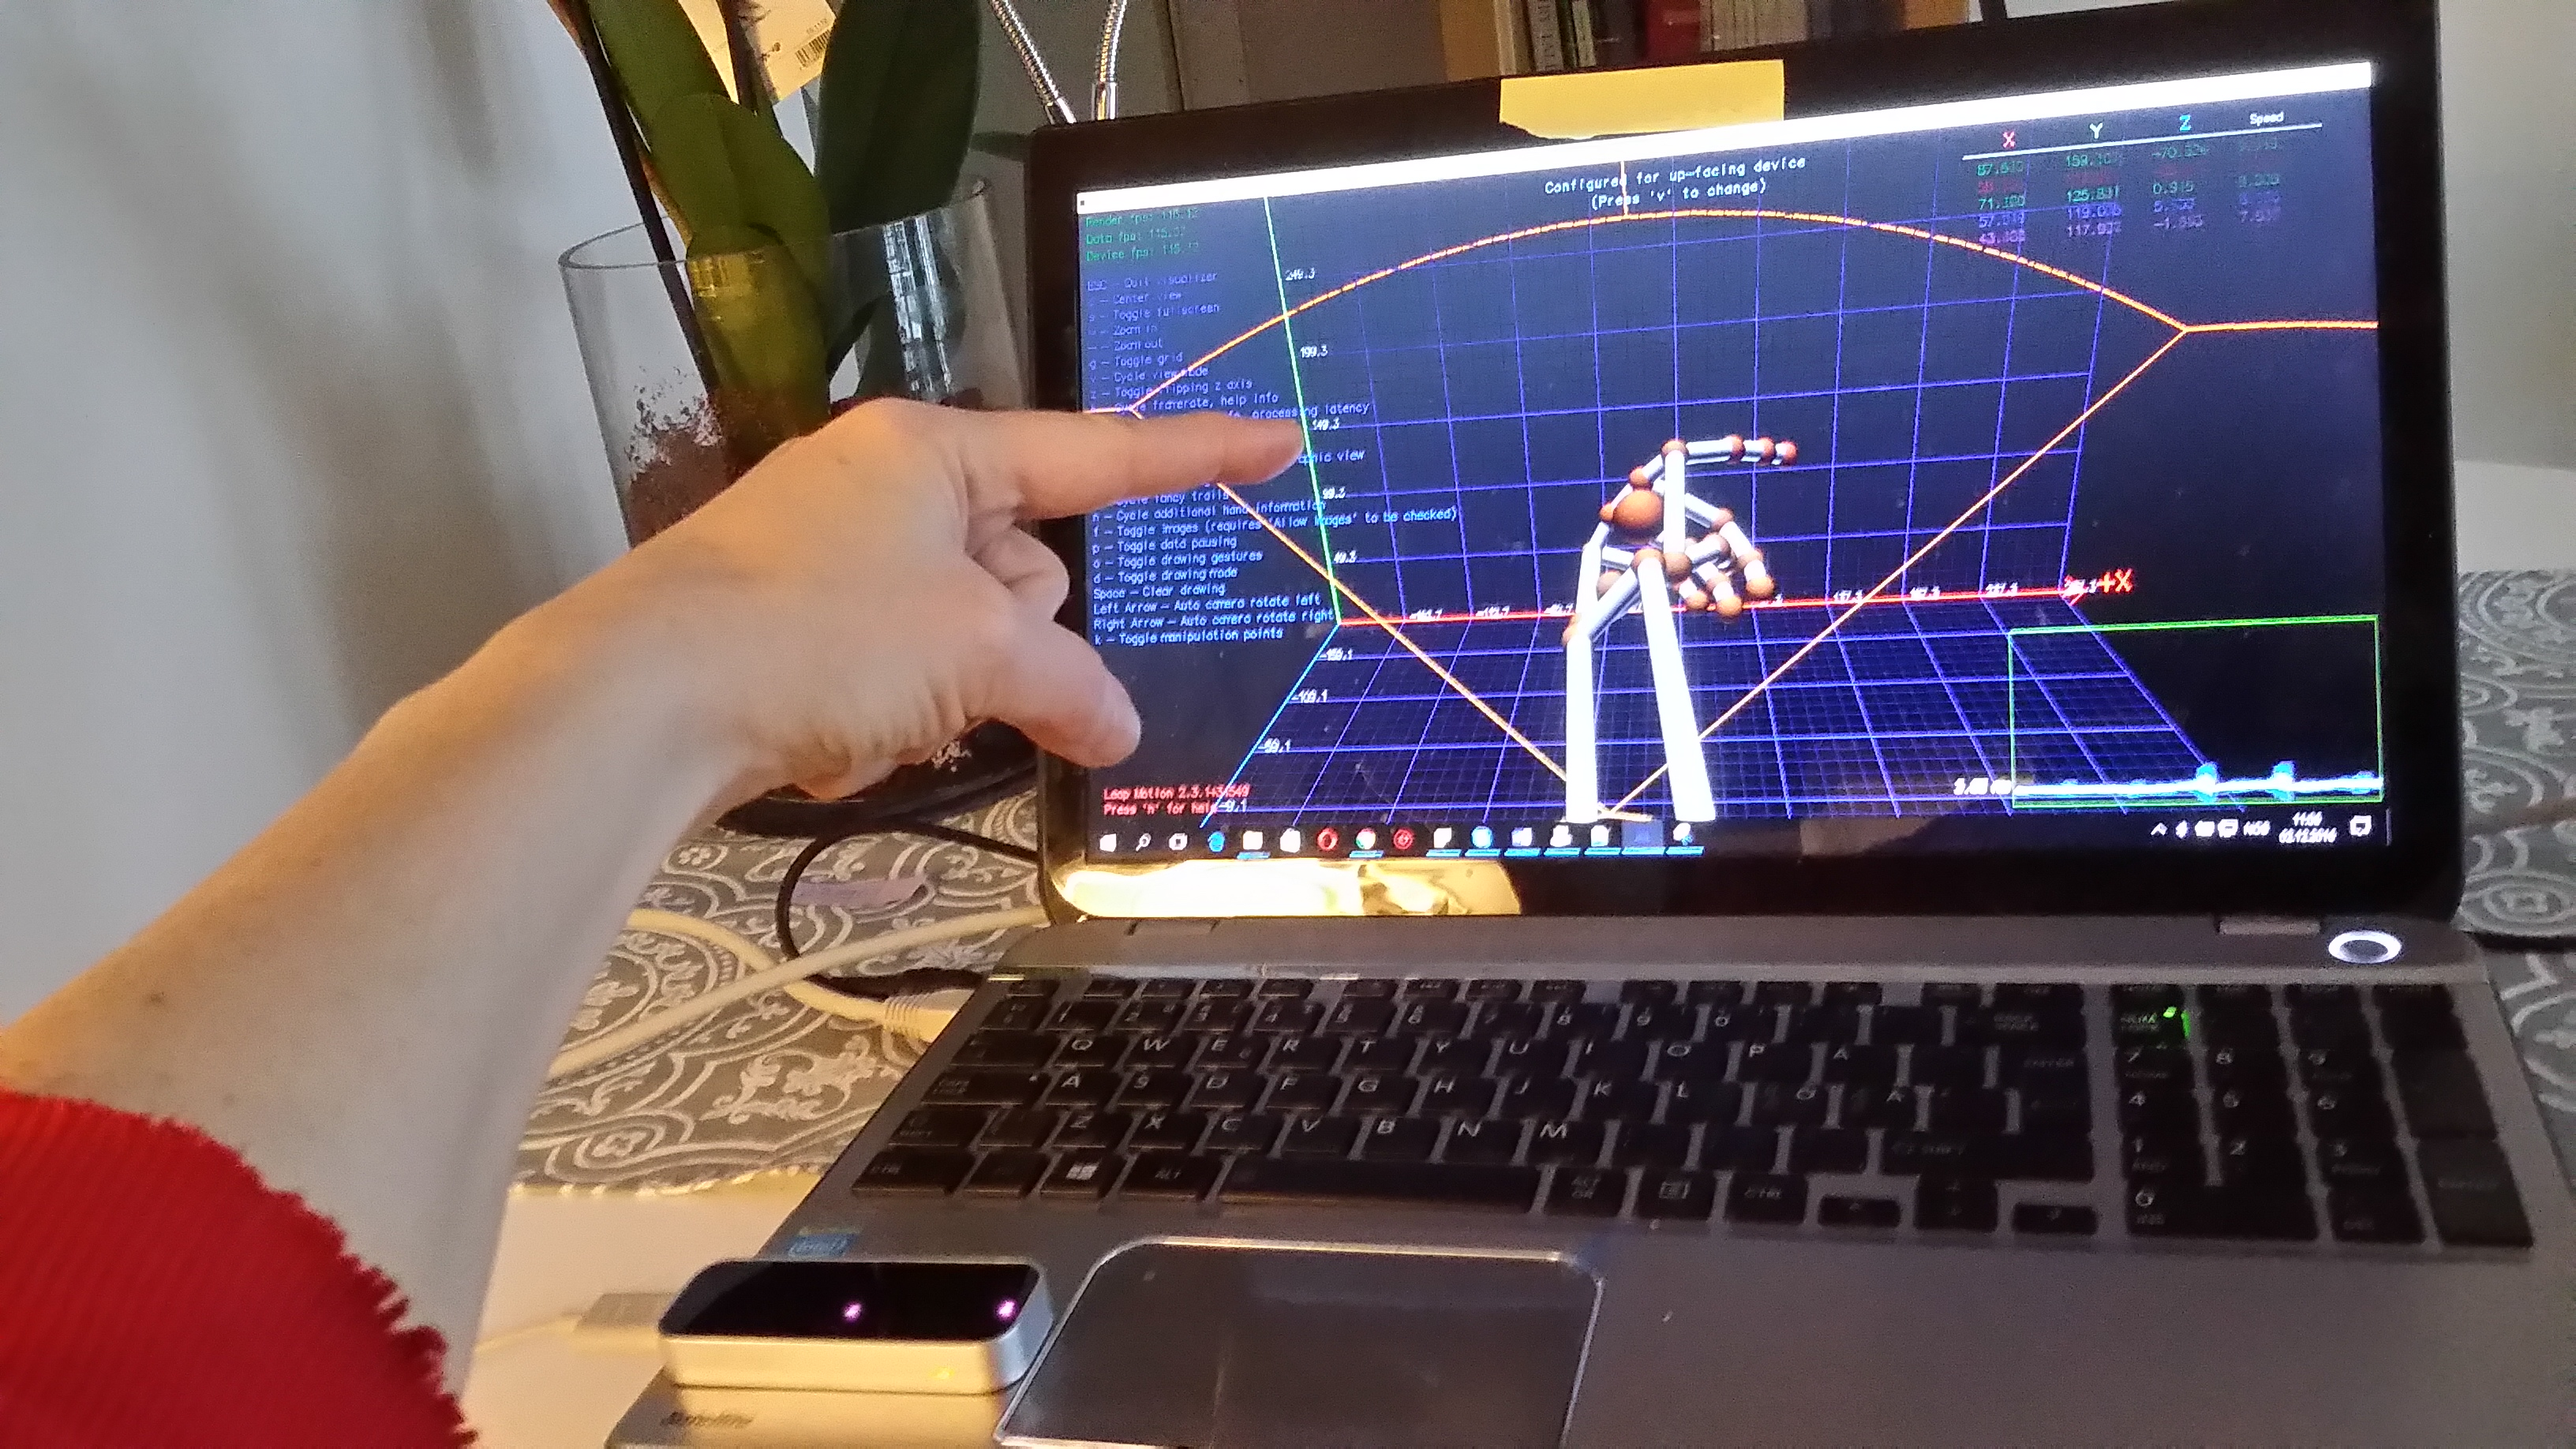
\includegraphics[width=.5\textwidth]{figures/LMvisualizer.jpg}
  \caption[Leap Motion visualizer.]{Leap Motion visualizer.}
  \label{fig:setup}
\end{figure}

The Java SDK documentation provided a good overview of the tracking data, hardware and software and showed how to get started with the Leap Motion API which was an excellent help during the whole prototyping process.

\subsection{Choosing a prototype tool}

A software prototype for test purpose was necessary to develop for this project. In order to accomplish the task it was essential to find a tool that could be used to create a simple and fast prototype and additionally is compatible with the Leap motion sensor. A quick Google search suggested Processing \footnote{https://processing.org/} which is a free open-source software. According to processing.org, the software is built particular within visual arts but also used for animation, installation products and interactive experience. It is a convenient prototype tool because it contains a integrated graphical user interface and additionally it is possible to use Java programming language in a simplified form.
Processing could also be used as a bridge between Leap Motion and Eclipse \footnote{https://eclipse.org/} which is known as an essential tool for Java developer.  Nevertheless, using Eclipse would be extensive and the setup would be more time consuming even if this would have been a more professional approach.

However, for this project, a simple and fast prototype was completely sufficient. For that reason, Processing was a suitable option. For the prototype development, Processing version 3.3.6 was installed locally.


\subsection{Game design}

In the initial design stage the idea of the whole system was sketched. In this stage the system had five modules. However, only one module could be implemented for this project due to the time limit.

\begin{figure}[h]  %t top, b bottom, p page | you can also use h to try to get the figure to appear at the current location
  \centering
  \includegraphics[width=.6\textwidth]{figures/sketch_wholeSystem.jpg}
  \caption[Idea generating.]{ Idea generating for the whole system}
  \label{fig:setup}
\end{figure}

For this project, the module "Mole in the hole" was chosen to implement further.

\begin{figure}[!h]  %t top, b bottom, p page | you can also use h to try to get the figure to appear at the current location
  \centering
  \includegraphics[width=.6\textwidth]{figures/prototypeSketch.jpg}
  \caption[Sketch Mole in the hole.]{Sketch: Mole in the hole}
  \label{fig:setup}
\end{figure}

At the second stage of the design process the background picture and figures needed to be created.The background picture was created in Adobe illustrator, version CS4. A photo illustrating the forest floor was downloaded free from Pixaby \footnote{www.pixaby.com} and used for the upper part of the game’s canvas. The underground was drawn as a vector art to make it more childlike. 
A grid was drawn and used as dimension and measurement aid for the white path. This was needed to simplify the programming implementation that used the same grid size. However, the grid was just an drawing aid and was not visible in the end product.

\begin{figure}[h]  %t top, b bottom, p page | you can also use h to try to get the figure to appear at the current location
  \centering
  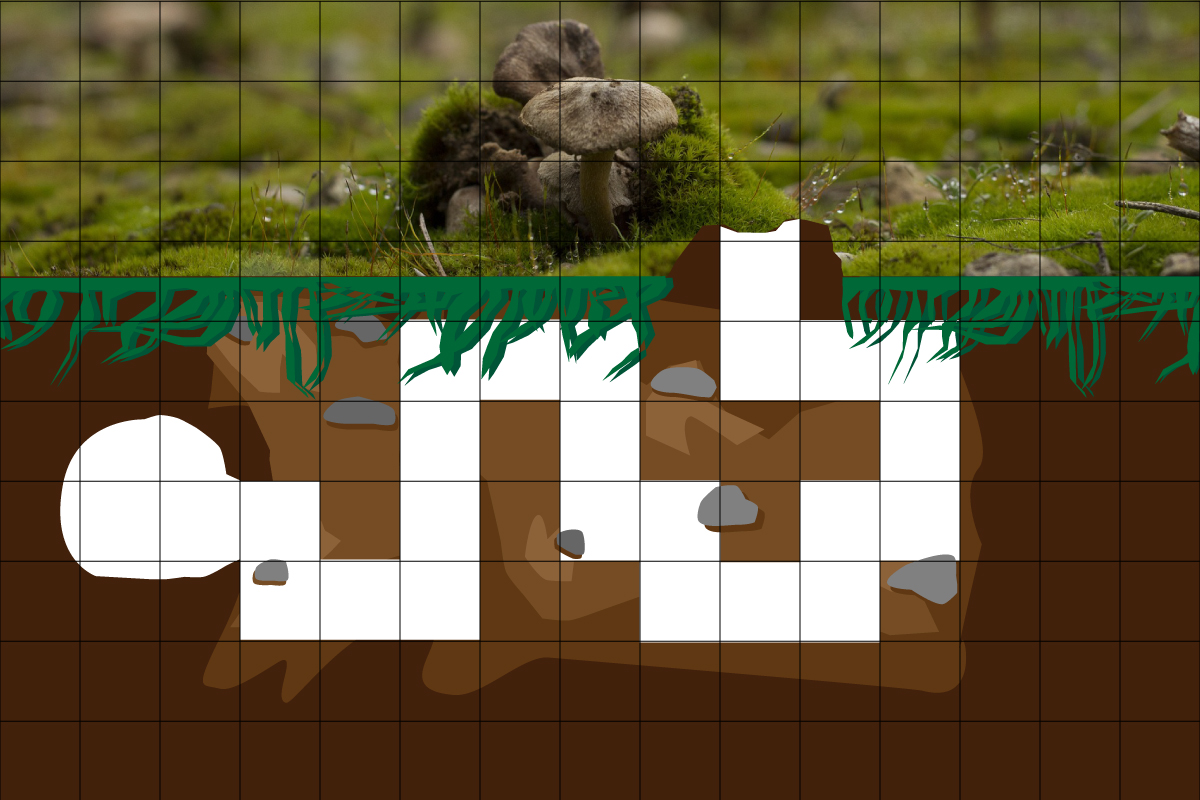
\includegraphics[width=.5\textwidth]{figures/Mole-in-the-hole-800x1200-GRID.jpg}
  \caption[Mole in the hole grid.]{Mole in the hole - grid.}
  \label{fig:setup}
\end{figure}

The five mole states and the stopwatch were drawn as a vector graphic in Adobe Illustrator, as well.

\begin{figure}[h]  %t top, b bottom, p page | you can also use h to try to get the figure to appear at the current location
  \centering
  
\includegraphics[width=.1\textwidth]{figures/MoleWait.png}
   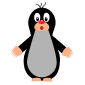
\includegraphics[width=.1\textwidth]{figures/MoleAttention.png}
   
\includegraphics[width=.1\textwidth]{figures/MoleJump.png}
   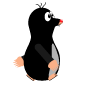
\includegraphics[width=.1\textwidth]{figures/MoleGo.png}
   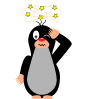
\includegraphics[width=.1\textwidth]{figures/MoleKaBoom.png}
  \caption[Mole's states.]{ The Mole's states: wait, attention, ready, go, hit.}
  \label{fig:setup}
\end{figure}

\begin{figure}[h]
  \centering
  
\includegraphics[width=.1\textwidth]{figures/timer.png}
  \caption[Timer]{Timer}
\end{figure}


The third design stage focused on illustrating the implementation and demonstrated the solution to the given problem.
A flow diagram was created for a better understanding of the design process and to analyze design problems. It illustrates the process stages and the conditions during the process from start point to the end point. 

\break

\begin{figure}[h]
    \centering
    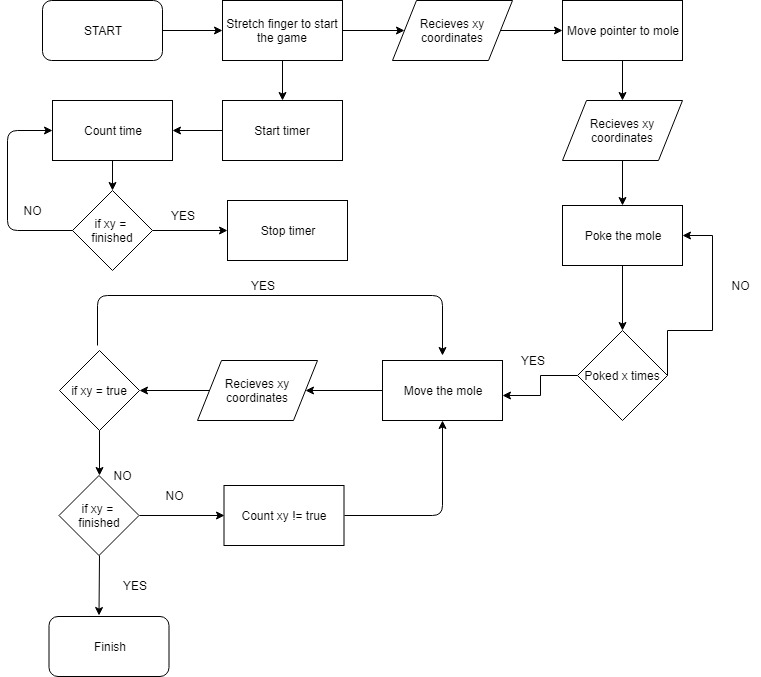
\includegraphics[width=.8\textwidth]{figures/FlowDiagram.jpg}
    \caption[Flow diagram: game design]{Flow diagram illustrates the game process}
    \label{fig: flowdiagram}
\end{figure}


\subsection{Prototype implementation}

In Processing, in order to make an animation or a interactive program, a predefined structure is used which includes a setup() and a draw() function. The setup() function runs only ones at the start whereas the draw() function loops continuously until the program is terminated or the noLoop() command appears in the code.
In the setup() function, the initial environment property as for instance the size of the canvas is defined  (size()).  In the draw() function, code that is meant to run continuously is defined here, like for instance the background() property. 

The framework would look likes this:
\lstset{frameround=tttt}
\lstset{frame=single}
\lstset{xleftmargin=.05\textwidth, xrightmargin=.05\textwidth}
\lstset{language=Java}
\begin{lstlisting}[caption = {Processing framework}, label={lst:Java}]
        void setup(
        {
            size();
        }
        void draw()
        {
            background();
        }

\end{lstlisting}

The program code for the module “Mole in the hole” implemented functions from the Leap Motion API. In order to use these functions the leap Motion library needed to be imported.

\lstset{language=Java}
\begin{lstlisting}[caption = {Leap Motion library}, label={lst:Java}]
import com.leapmotion.leap.*;
\end{lstlisting}

To connect to the Leap motion device a controller object was created

\lstset{language=Java}
\begin{lstlisting}[caption = {The code for touch zone}, label={lst:Java}]
Controller leap;
\end{lstlisting}

In setup() the controller was initialized as followed in order to establish a connection.

\lstset{language=Java}
\begin{lstlisting}[caption = {The code for touch zone}, label={lst:Java}]
leap = new Controller();
\end{lstlisting}

In order to make it easier to map position in the Leap Motion coordinate system an interaction box was initialized. The position within the 2D coordinate system was defined as X, Y which are coordinates for the hand and finger position. 

\lstset{language=Java}
\lstset{breaklines=true,postbreak=\mbox{{\color{blue}\tiny$\rightarrow$}}}
\begin{lstlisting}[caption = {The code for touch zone}, label={lst:Java}]

InteractionBox iBox = leap.frame().interactionBox();
Pointable pointable = leap.frame().pointables().frontmost();
Vector normalizedPosition = iBox.normalizePoint(pointable.stabilizedTipPosition());
float pixelX = normalizedPosition.getX() * windowWidth;
float pixelY = windowHeight - normalizedPosition.getY() * windowHeight;
int cx = (int) pixelX - 10;
int cy = (int) pixelY - 100;

\end{lstlisting}

Finger are recognize by the pointable class. The pointable.Zone defines the state of the current pointable object.

\lstset{language=Java}
\begin{lstlisting}[caption = {The code for touch zone}, label={lst:Java}]
 Pointable.Zone fingerzone = pointable.touchZone();
\end{lstlisting}

The touch zone is defined by three states:(see Leap Motion API reference for more information)
\begin{enumerate}
    \item ZONE\_NONE (pointable distant from the touch panel)
    \item ZONE\_HOVERING (is near the touch plane)
    \item ZONE\_TOUCHING (penetrates the touch plane)
\end{enumerate}




\lstset{language=Java}
\begin{lstlisting}[caption = {The code for touch zone}, label={lst:Java}]

            switch (pointable.touchZone()){
            case ZONE_NONE:
              //Handle distant pointable
              image(MoleState1, 80, 480);
              break;
            case ZONE_HOVERING:
              //Handle pointable near touch plane
              hide(MoleState1);
              image(MoleState2, 80, 480);
              break;
            case ZONE_TOUCHING:
              //Handle pointable penetrating touch plane
              counterTouching = counterTouching + 1;
              image(MoleJump, 80, 480); 
              break;
            default:
              //Handle error cases...
              break;
            }//end switch
          
\end{lstlisting}

A new finger object is created and initialized that starts the timer:

\lstset{language=Java}
\begin{lstlisting}[caption = {The code for touch zone}, label={lst:Java}]
  Finger finger = new Finger(pointable);
  if(finger.isExtended())
  {
    Timer(1);
  }
\end{lstlisting}

\break
%\break
In this game an invisible grid was drawn over the whole canvas size. Each grid cell had a size of 80 x 80 px. The mole’s hole and the way out was marked with white cells which x-y coordinates were stored as true-value in a two dimensional array.

\begin{figure}[h]  %t top, b bottom, p page | you can also use h to try to get the figure to appear at the current location
  \centering
  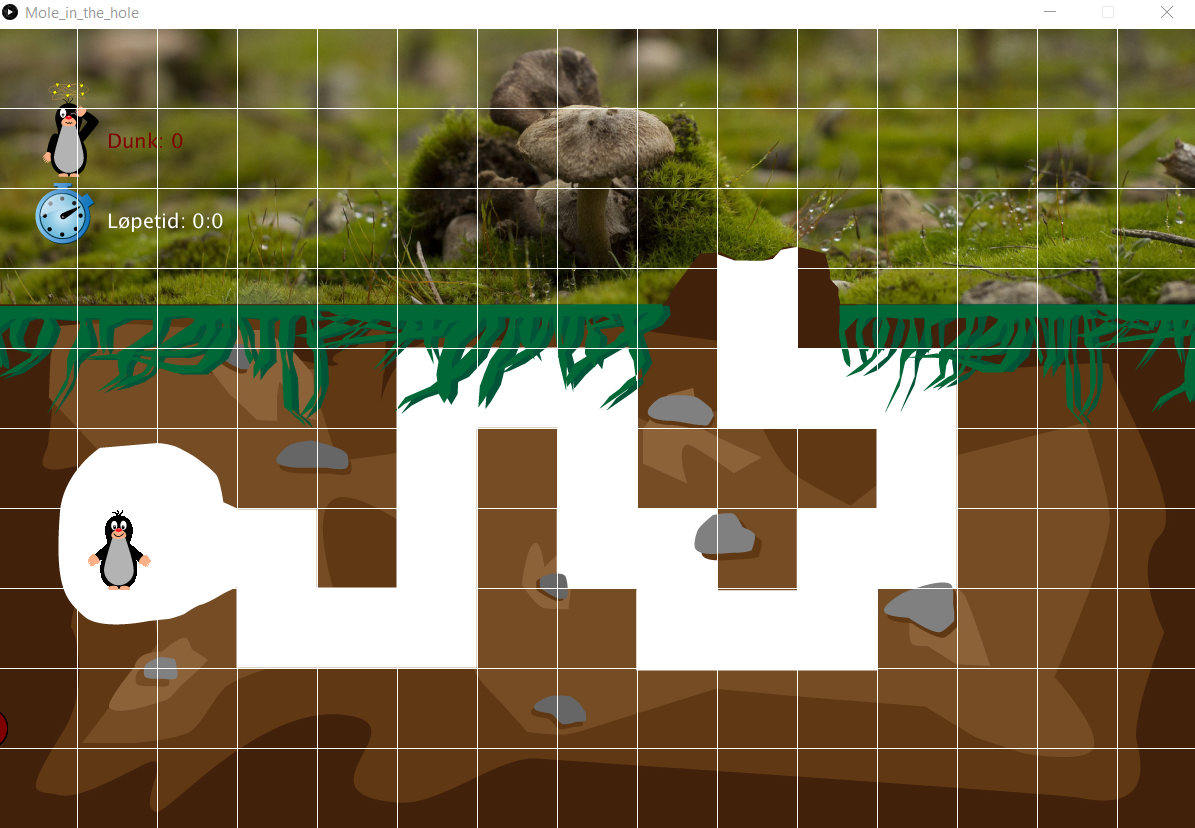
\includegraphics[width=.5\textwidth]{figures/Grid-processing-Mole_in_the_hole.png}
  \caption[Mole in the hole grid processing.]{Mole in the hole. Grid is drawn with a for loop.}
  \label{fig:setup}
\end{figure}

The pointer is activated by stretching the finger and pointing forward. The point moves in relation to the finger’s x,y coordinate. When the pointer hovers the mole, the mole changes state from “wait” to “attention”. When the Hole is poked his state will change from “attention” to “ready”. It needs about two til three pokes until the mole state changes to “go”. From that point the pointer disappear and only the mole moves and follows the finger’s position. All moves that are defined as false are counted as “hit”. The games is finished when the mole reaches the exit. The game counts the amount of hits and the elapsed time. The timer starts when the finger is stretched and the participant is ready to go.

\begin{figure}[h]  %t top, b bottom, p page | you can also use h to try to get the figure to appear at the current location
  \centering
  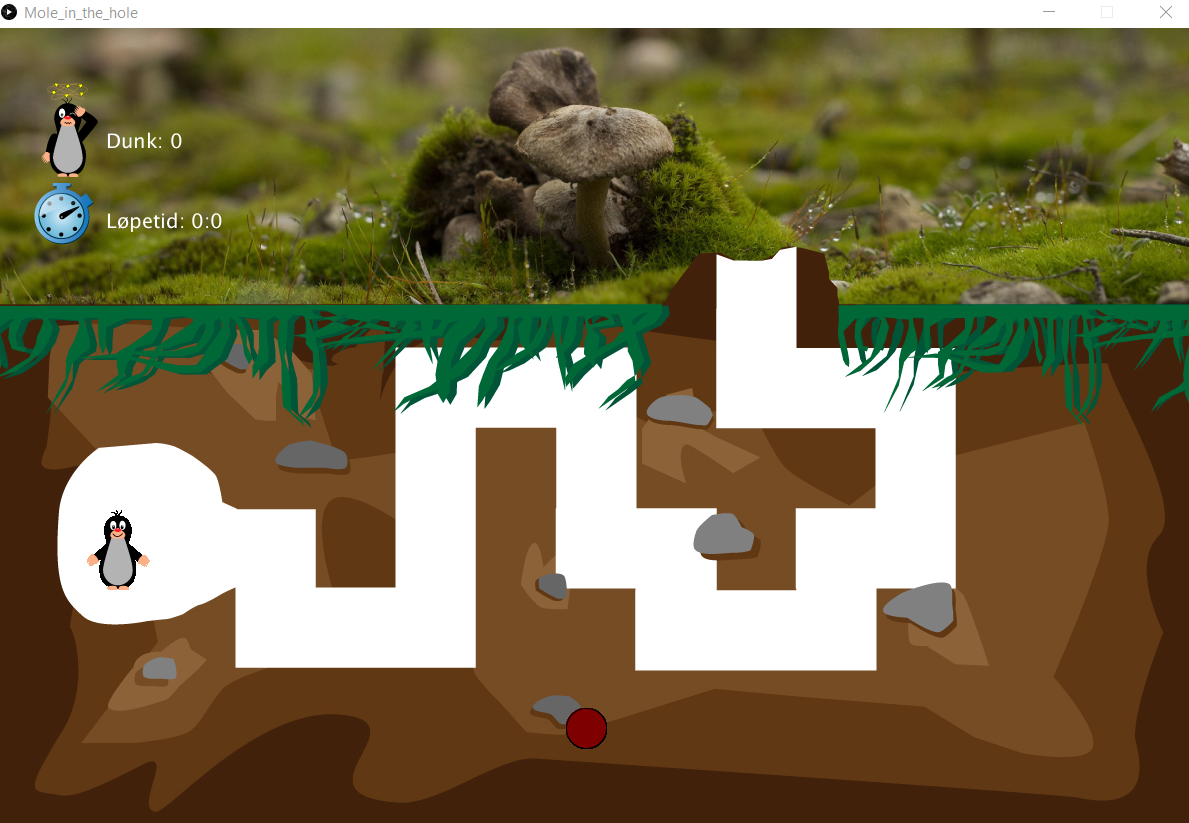
\includegraphics[width=.5\textwidth]{figures/StateStart-Mole_in_the_hole.png}
  \caption[Mole in the hole state start.]{Mole in the hole. State: start.}
  \label{fig:setup}
\end{figure}
\begin{figure}[h]  %t top, b bottom, p page | you can also use h to try to get the figure to appear at the current location
  \centering
  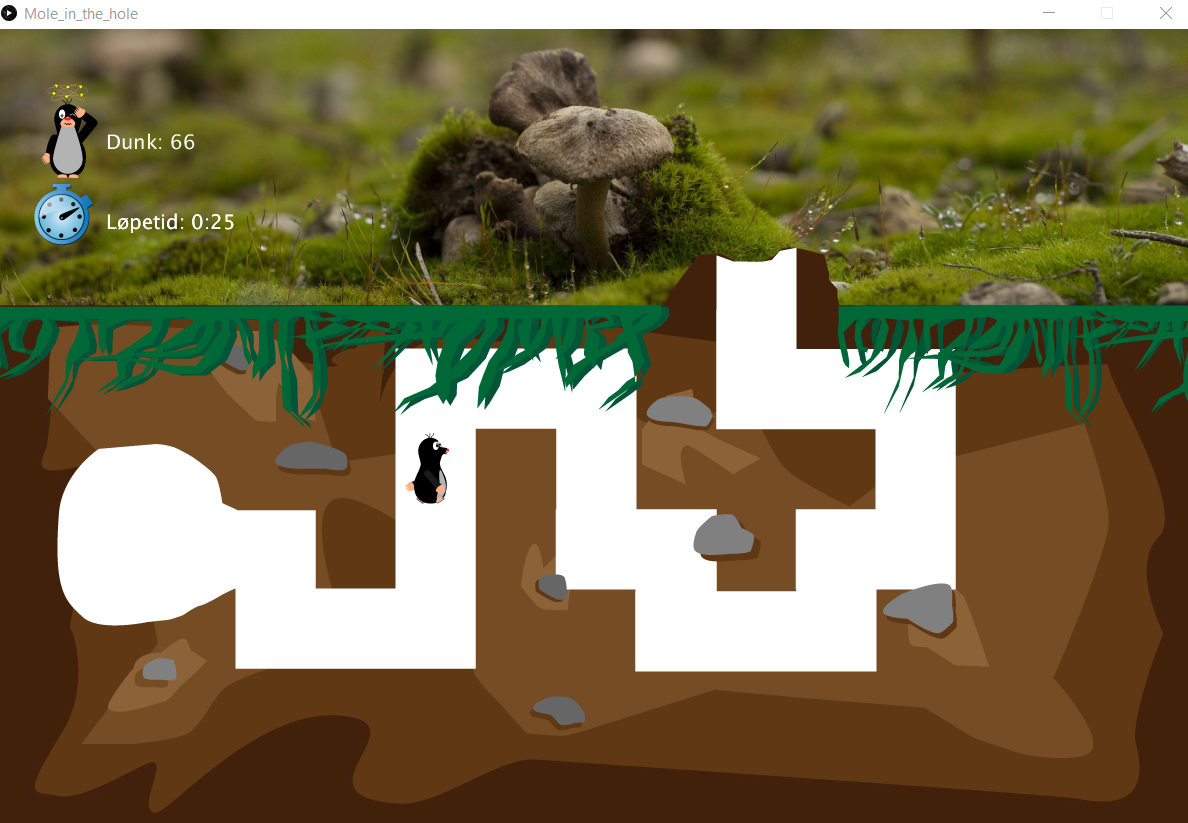
\includegraphics[width=.5\textwidth]{figures/StateGo-Mole_in_the_hole.png}
  \caption[Mole in the hole state go.]{Mole in the hole. State: go.}
  \label{fig:setup}
\end{figure}
\begin{figure}[h]  %t top, b bottom, p page | you can also use h to try to get the figure to appear at the current location
  \centering
  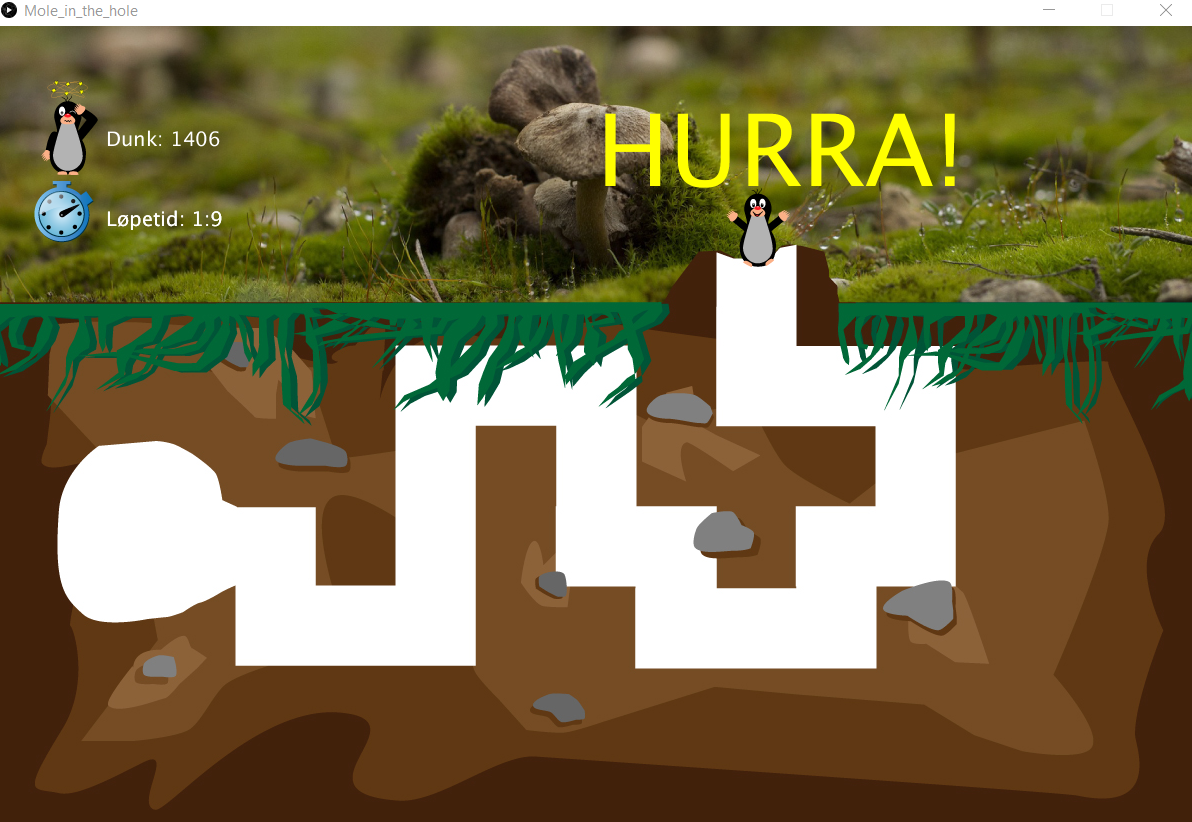
\includegraphics[width=.5\textwidth]{figures/EndState_Mole_in_the_hole.png}
  \caption[Mole in the hole state end.]{Mole in the hole. State: end.}
  \label{fig:setup}
\end{figure}



\subsection{Limitation}
time limit
money? budget
poor code quality
equipment limitation

\section{Experiment }
\label{sec:experiment}


\subsection{Recruiting participant}
\label{sec:participant}

The target group for this study were children between two and 13 years of age. A suitable combination of gender distribution would be appropriate for the usability test. For this purpose, convenience sampling of children that were readily available represent a subset of the population. A social network as recruiting source was substantial in this situation. Parents who saw the value of this study wanted to contribute and volunteered their children. 
The motive behind such young target group is, to observe and analyze if the child understands the idea a touch-less system and the ability to handle it. 

According to www.usertest.com, it is recommend to divide children into specific age groups. The main reason for that is the remarkable differences in development of cognitive, physical and social skills. For instance, fine-motor skill are less developed in a 3 year old child than i an a 10 year old. The user group in this study can be divided into group 1 (age 2 - 4), group 2 (age 5 - 8) and group 3 (age 9 -1).

The planed number of participant for the usability study was between nine and ten children. Since the study focused on qualitative data collection and Nielsen recommends 5 users for usability test, the amount of users were sufficient for this study. That would be a sufficient backup in case a child did not want to cooperate or if a child got ill. 


\subsection{Test environment and implementation strategy}
\label{sec:environmnent}

The project is about gaining meaningful data from a gesture-based application when screening children for fine motor deficiency
Working with children can be fun but also challenging at the same time. It needs a certain sensitivity and understanding of children's behaviour and feelings. Children can feel insecure  and anxious in a new environment which could make testing more stressful which probably would result in a wrong outcome. For that reason, each test was conducted at the child's home - a familiar and save environment. Since the equipment was portable, changing the test environment for each participant was not a concern.
Furthermore, in order to gain meaningful data from the experiment, a child's cooperation was necessary.  After a long day at daycare or at school, kids are usually tired and unfocused and hard to motivate. That is especially the case of younger children. For that reason, the experiments were carried out during the weekend and public holidays.  

The time duration needed to complete the task was estimated to 15 minutes. That included 3 attempts and answering the follow up questions. Additionally, extra 20 - 30 minutes were planned for presentation, introduction, equipment setup, debriefing and final thank-you-conversation.

\subsection{Compensation}

According to Nielsen [1998], compensating test users is common. The value of the compensation depends on the type of study and participants. However, he suggested a nice toy or 10 - 15\$ for children or students.
In this study, every child got a small compensation for their contribution. A collection of toys, games, book and other things were offered to choose from. This showed to be a good motivational tool and the children were eagerly to participate and accomplished the task.  

https://www.nngroup.com/articles/when-to-outsource-recruiting-test-users/



\subsection{Equipment}

The equipment for the experiment consisted of a laptop, an external screen and a gesture sensor (Leap Motion). 

\begin{figure}[h]  %t top, b bottom, p page | you can also use h to try to get the figure to appear at the current location
  \centering
  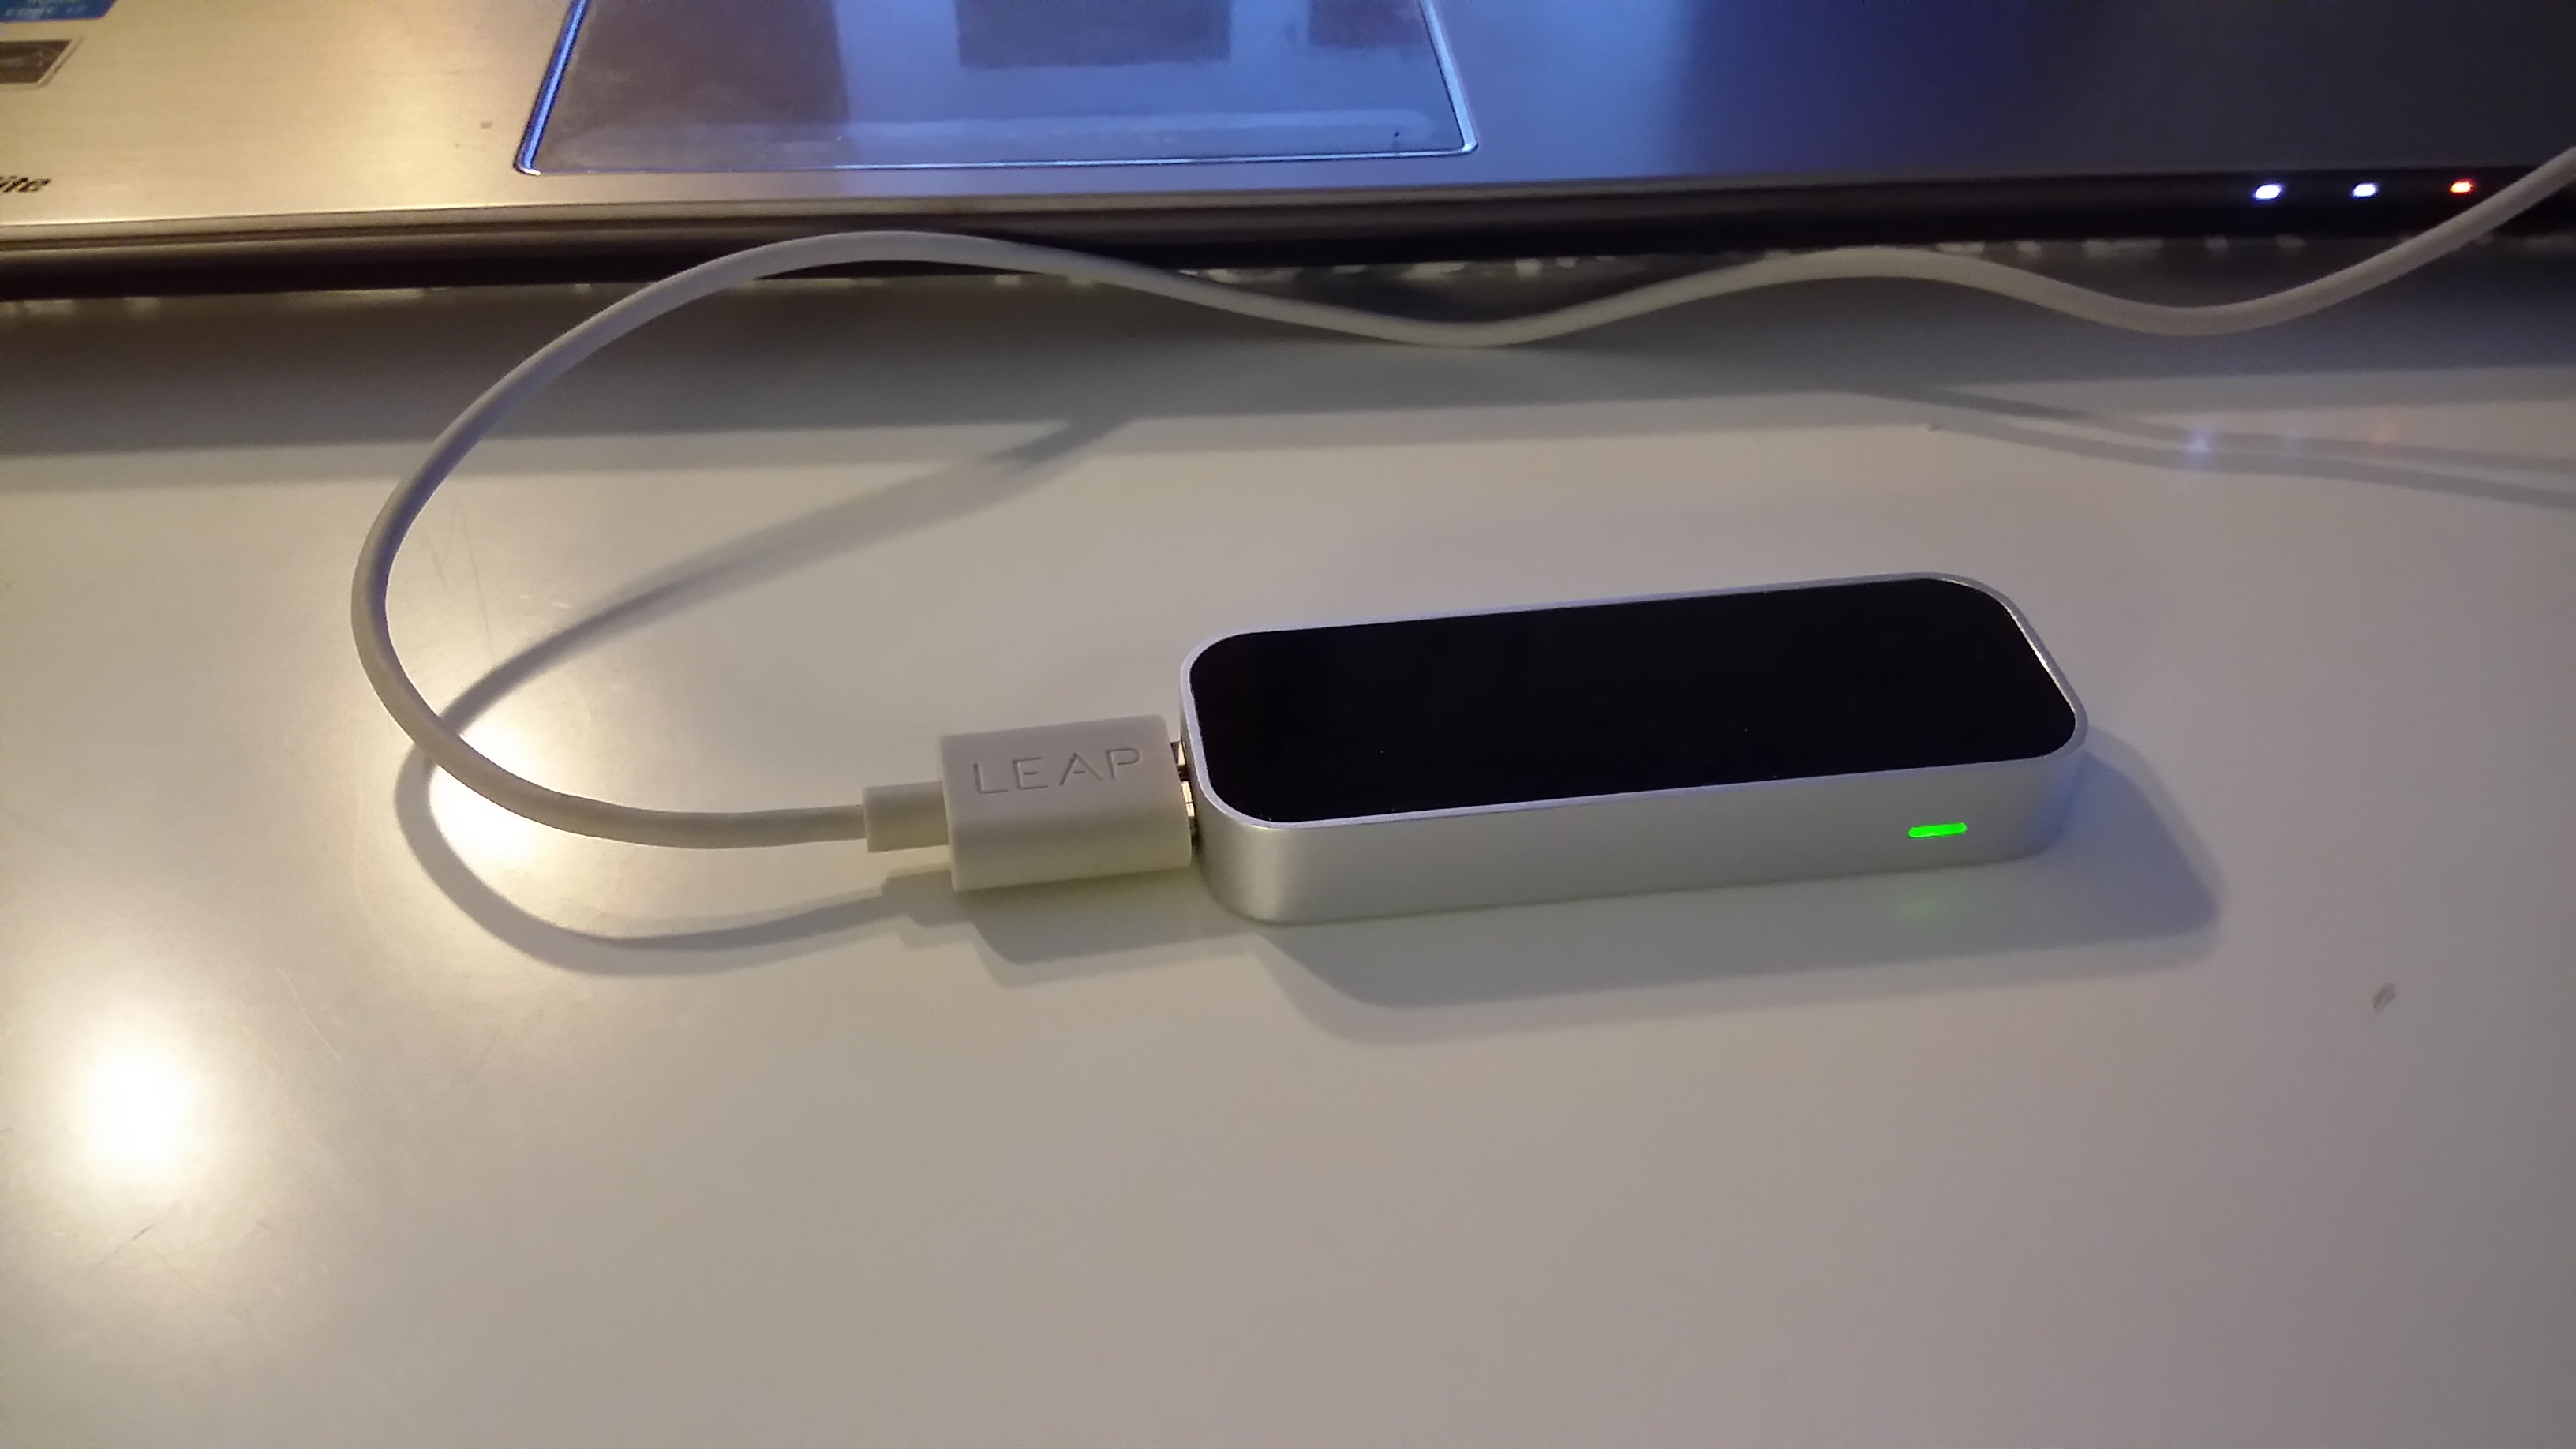
\includegraphics[width=.5\textwidth]{figures/LMdevice.jpg}
  \caption[Leap Motion device.]{Leap Motion device.}
  \label{fig:setup}
\end{figure}

The set up of the equipment needed to be straight forward and fast. An external screen and the Leap Motion device were placed on the table in front of the child. Both, screen and scanner were connected to the laptop. The laptop was place in a way so that the laptop’s screen was not in vision of the test person. All sound that could disturbed during the test session was turned off and the test person could so focus completely on the task.

\begin{figure}[h]  %t top, b bottom, p page | you can also use h to try to get the figure to appear at the current location
  \centering
  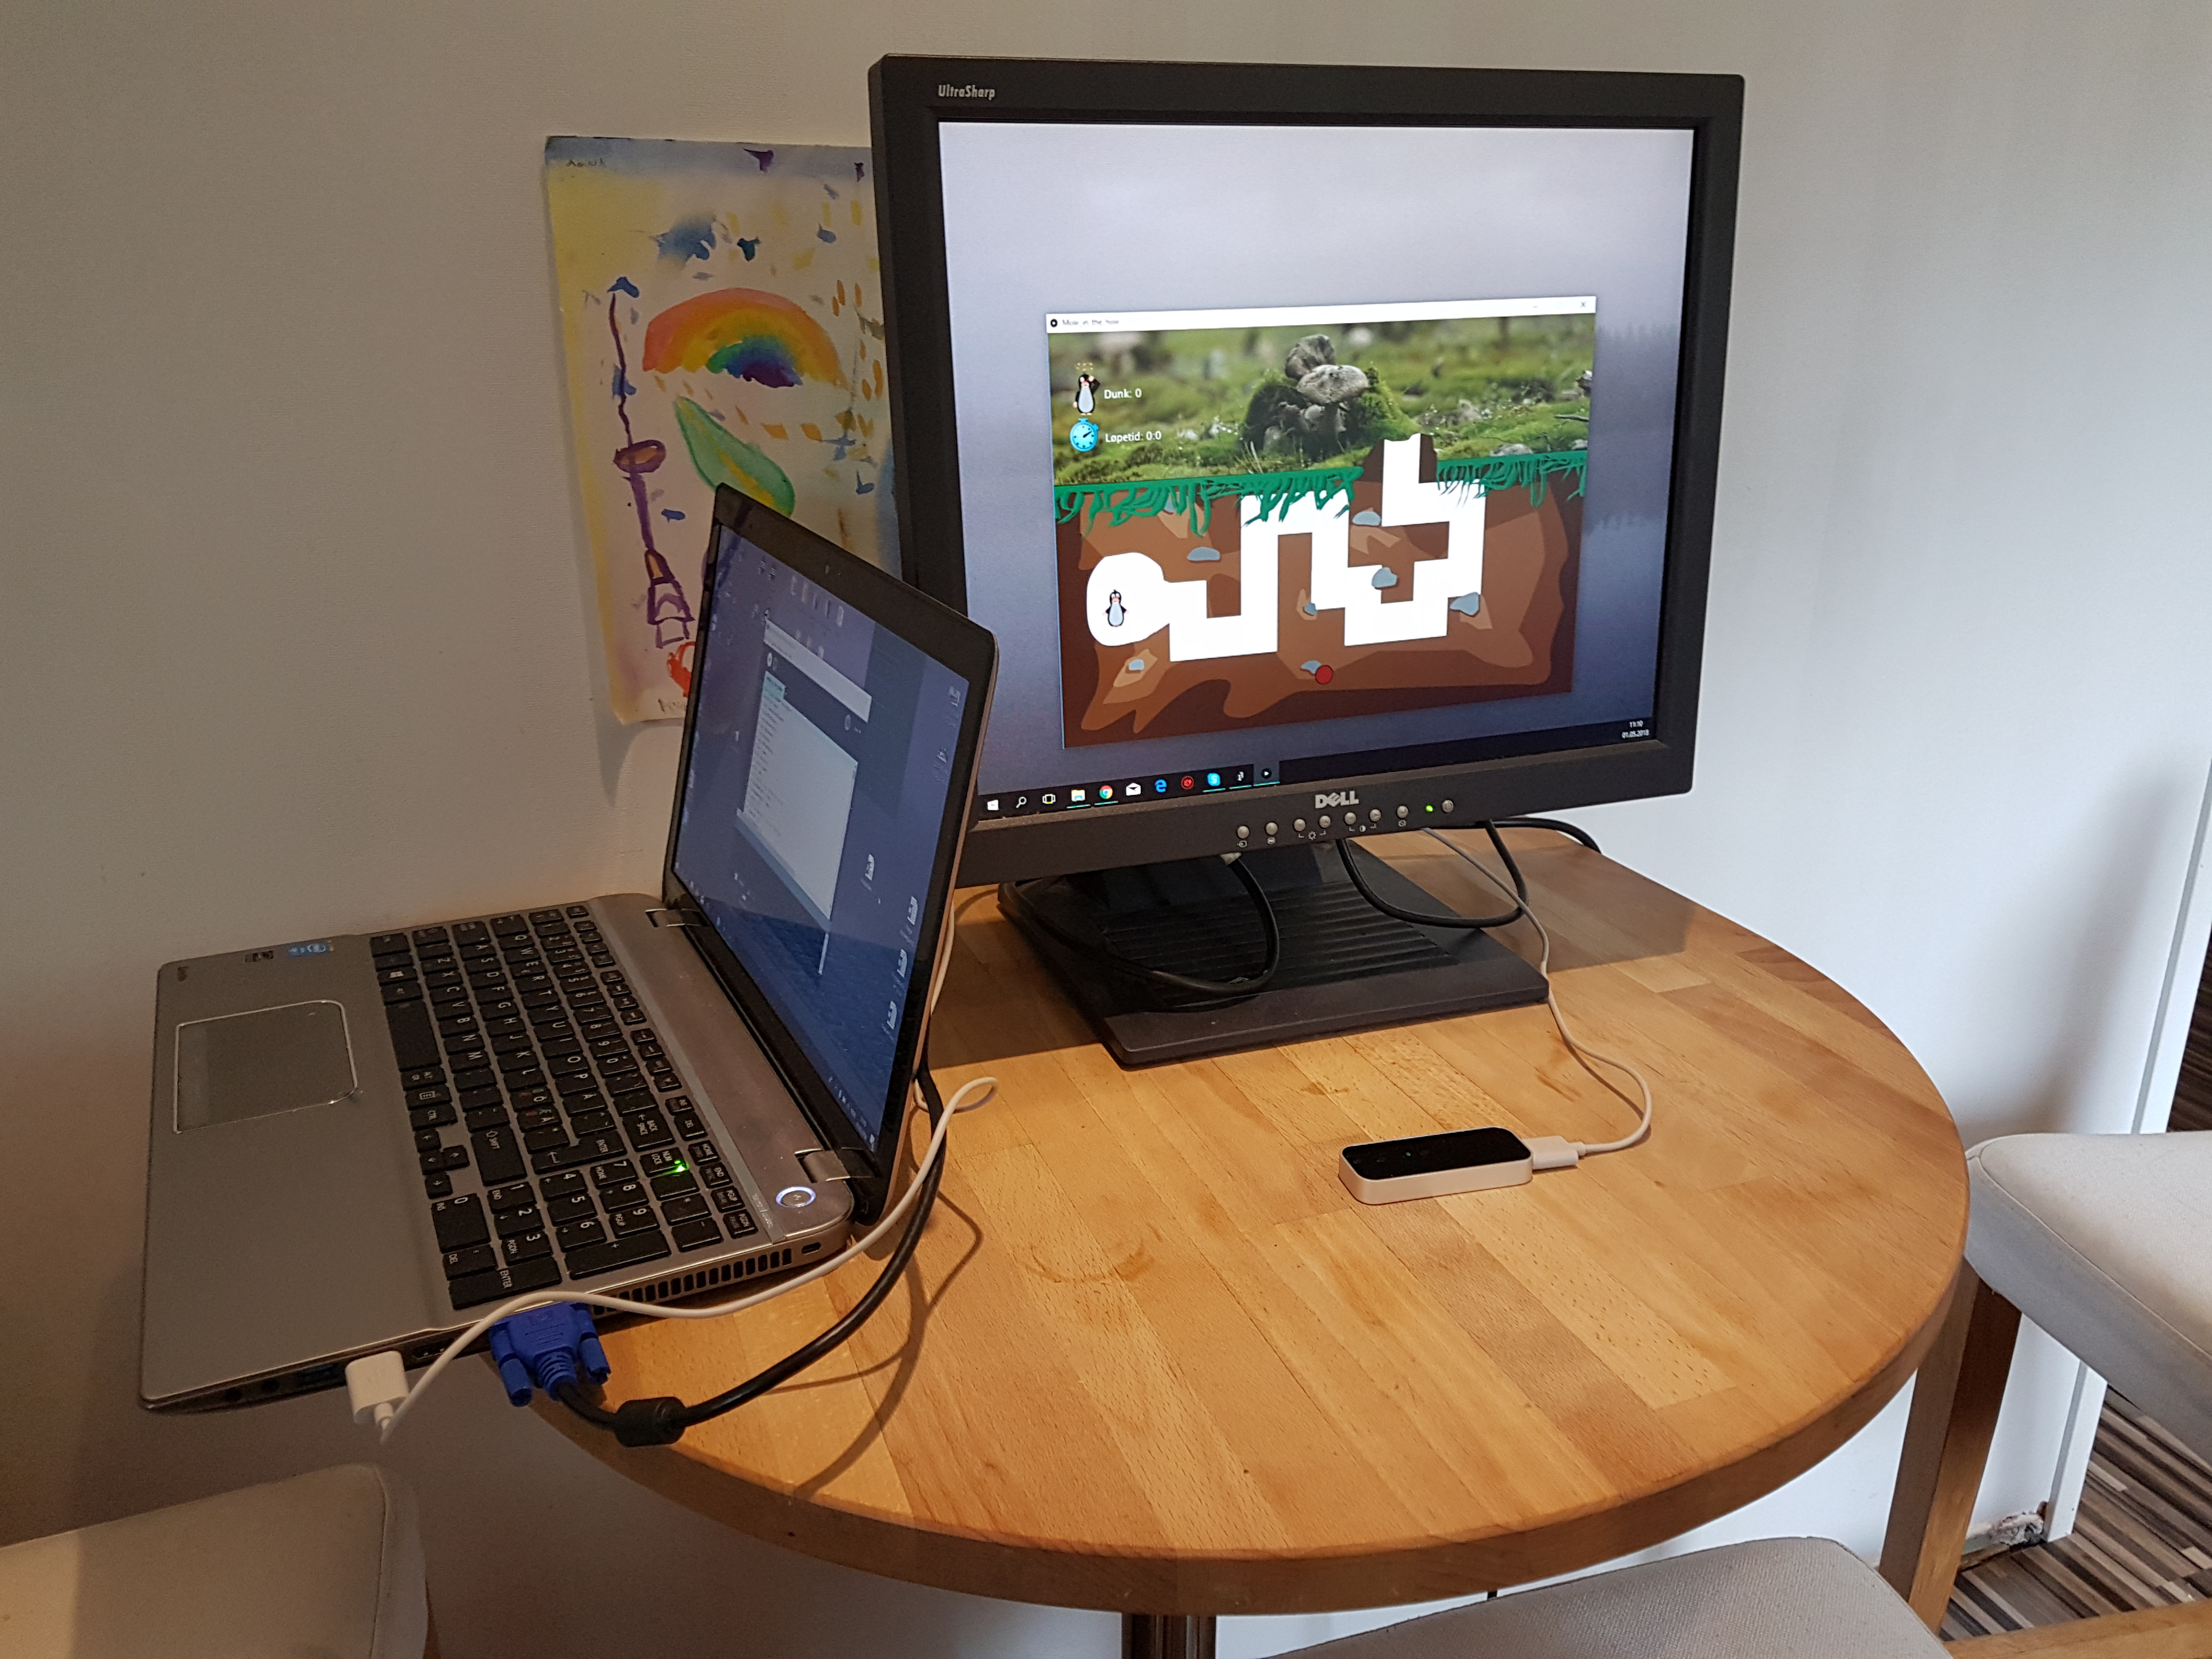
\includegraphics[width=.5\textwidth]{figures/setup.jpg}
  \caption[Equipment setup.]{Equipment setup.}
  \label{fig:setup}
\end{figure}


\subsection{Ethical consideration}
\label{sec:ethical}

Studies involving human participants require considerations of ethical aspects. Children in particularly have to be protected from doubtful research. In this study, ethics, confidentiality and privacy was an important factor during the whole project.
During the experiment, the children were never forced to carry out the task. All involvement was based on voluntary participation. If for any reason a child wasn't cooperative the experiences was canceled immediately. 
It is important to point out that the study didn't collect any personal data. Every participant was registered with a consecutive number which would not reveal the participant identity. The collected data was kept confidential. Only the overall outcome was used for further analysis in order to confirm the hypothesis.  

A concern form was handed to the parents to confirm and sign. The form was downloaded from www.usability.gov and modified for this study. (see attached concern form)


\subsection{Pilot test}

A pilot test was conducted before the real test in order to fine-tune the prototype and test routine and to check if there a other issues to be considered. 
https://www.nngroup.com/articles/pilot-testing/

The person recruited for the pilot test was a young girl in her early teens. She had no pre-experience in hands free gesture applications and was therefore suitable for the task.
The pilot test was conducted some days before the real test.

\begin{figure}[h]  %t top, b bottom, p page | you can also use h to try to get the figure to appear at the current location
  \centering
  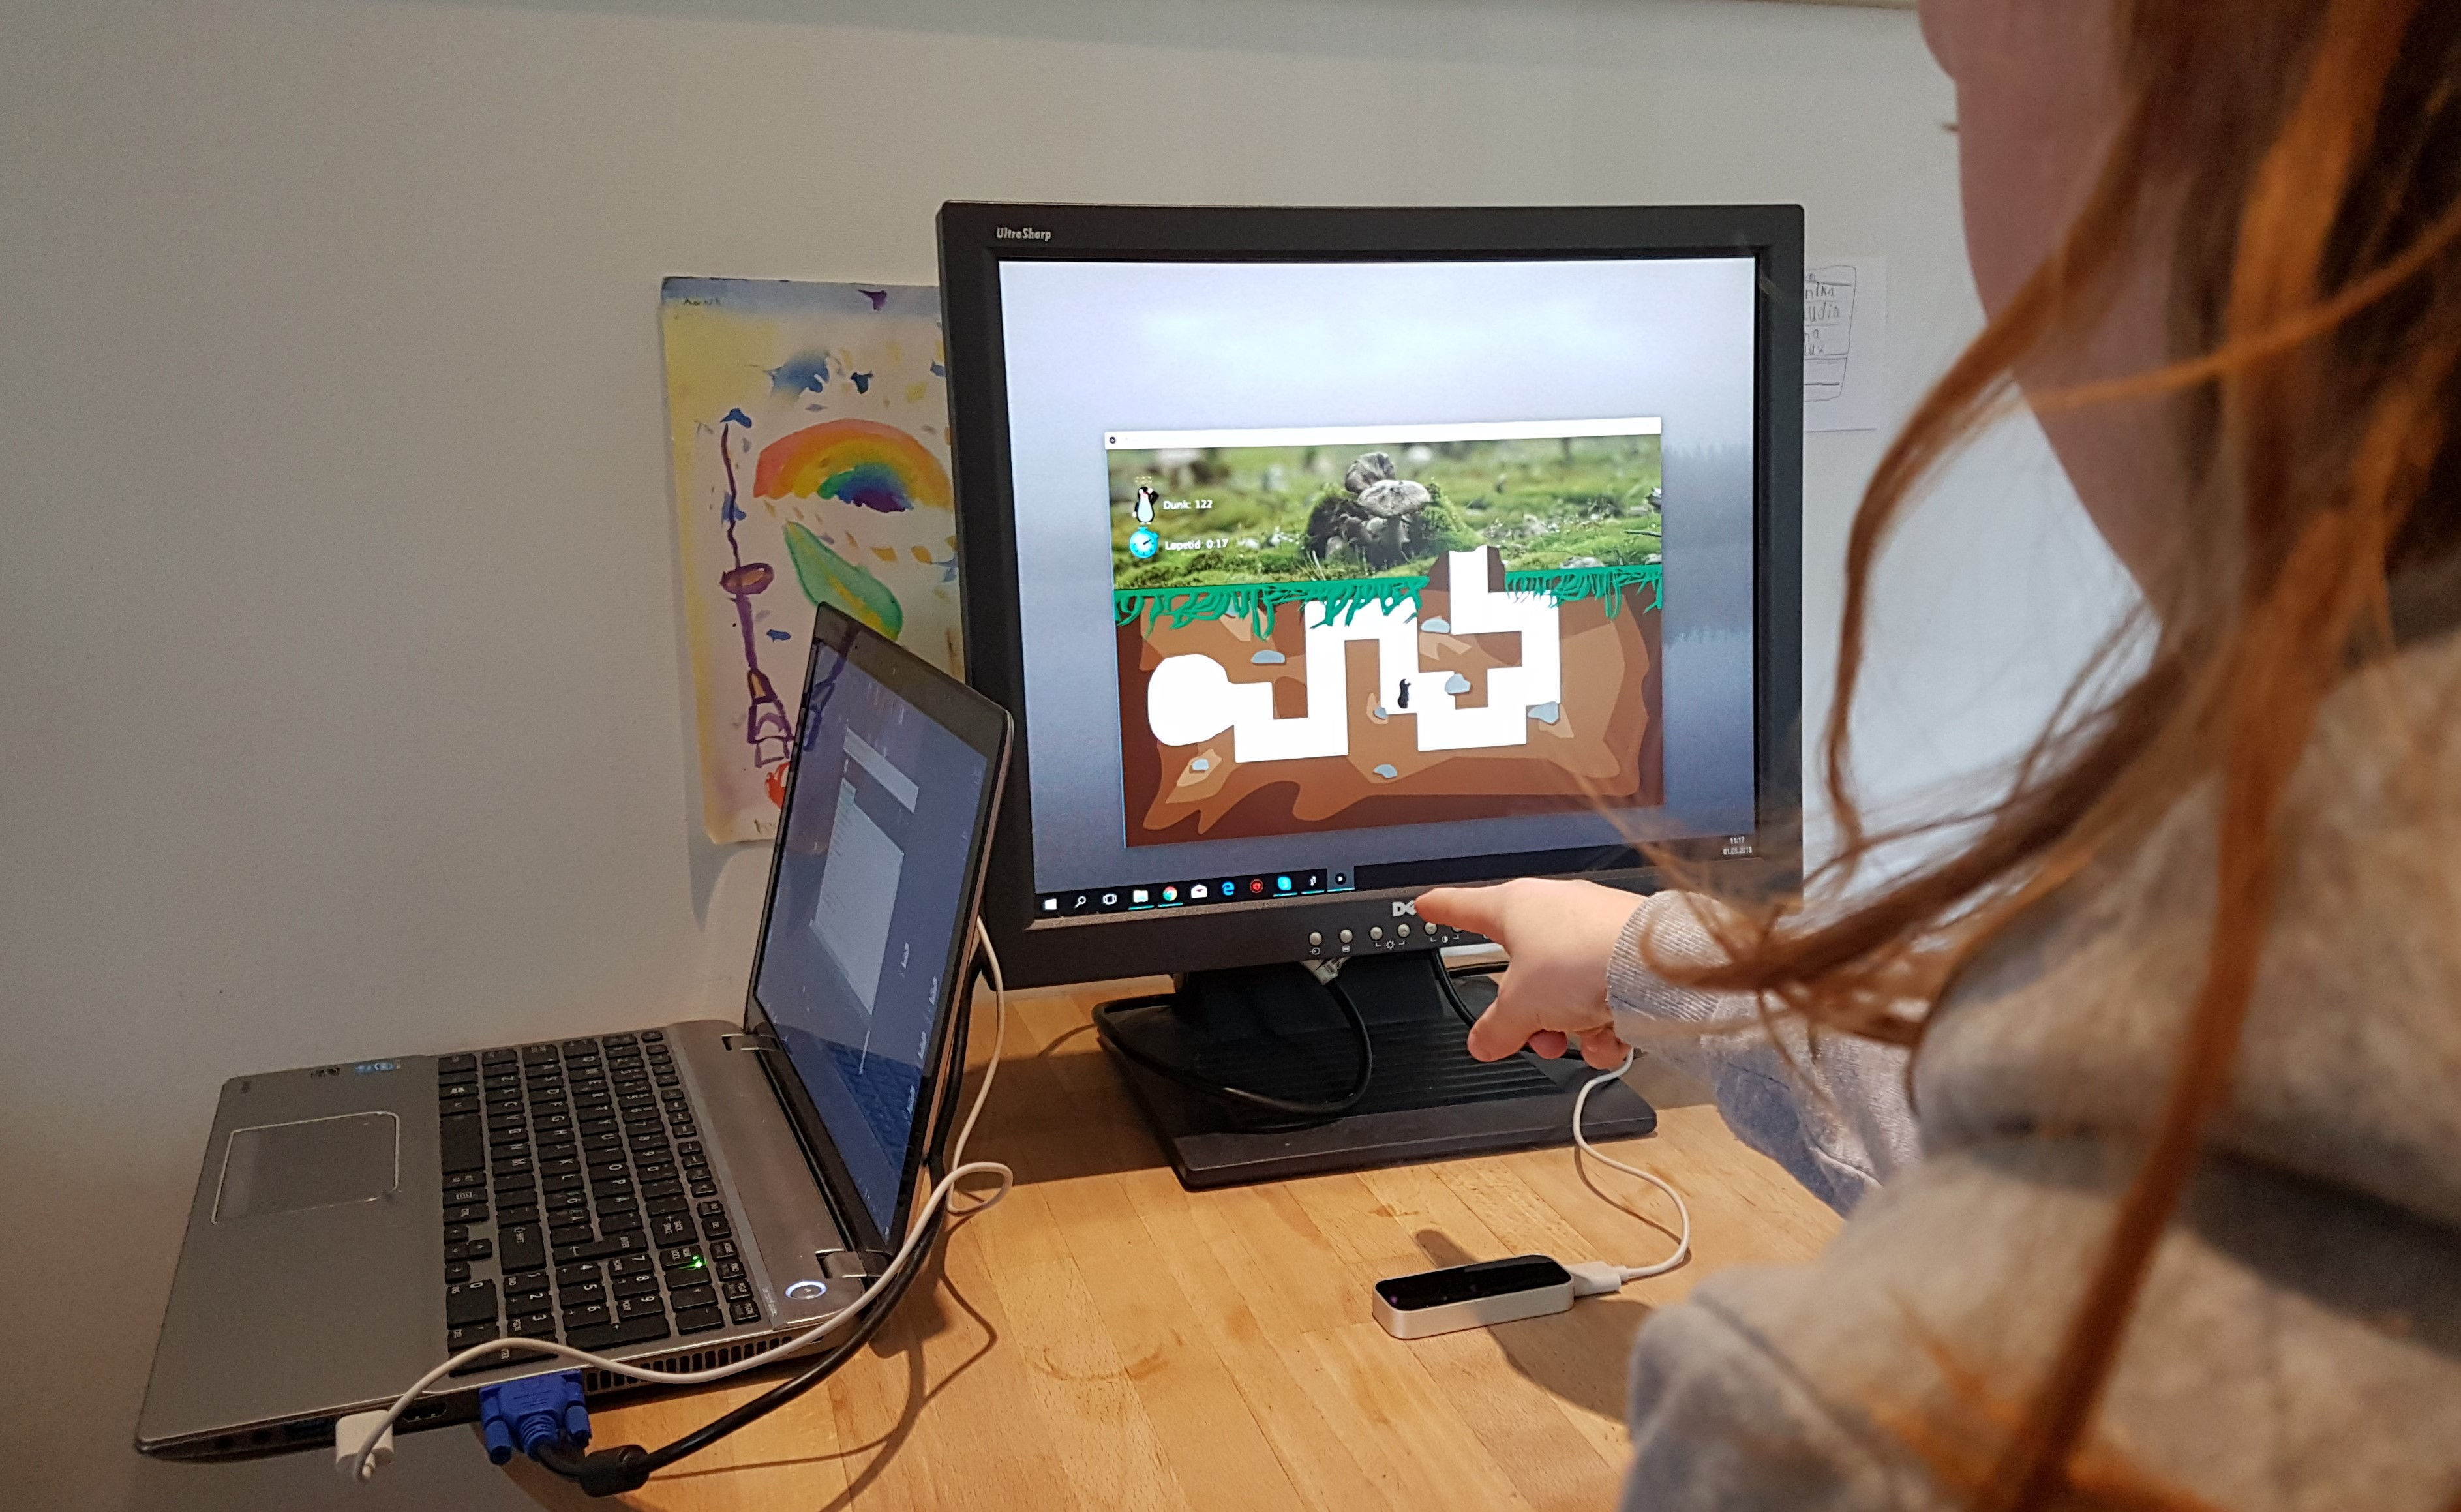
\includegraphics[width=.5\textwidth]{figures/pilottest.jpg}
  \caption[Pilot test.]{Pilot test.}
  \label{fig:setup}
\end{figure}

The pilot test revealed some few issues that needed to be improved or at least to be considered in the real test.  One of the issues concerned the understanding of the system. Since the freehand sensor is a device that still is quite unknown to children,  it is  not enough to say what the participant has to do, but it is  essential to show in advanced how the application works.

The second issue that needed to pay attention is the smiley scale. Since there are different smiley for the scales. Hard-easy and good - bad. It was not a good idea to have them all laid out in front of the participant since this leads to confusion.

The test showed that is was a good idea to have an external screen that only showed the application. 

Furthermore, the test reveal that it is an advantage if the table and the chair have a proper proportion and stands  in relation to the child's body high.

 
The pilot test confirmed the estimated time of 15 minutes of a test run. Additionally 15 min to build up the equipment, have a little conversation with the child, and debriefing.

\subsection{Task description and execution of the usability study}

The purpose behind the usability study was to investigate if the children understand the idea of hand-free interaction. Additionally, the extracted parameters served further analysis. The idea behind that, was to consider a hand-free interaction for medical examination and diagnostic tool. The task of the usability study was about moving the pointer to the mole and than move the mole to the exit as fast as possible while staying on the white path.
The kids also had to perform two gestures in additional, a pointer gesture and a poke gesture. The pointer gesture was needed to navigate and control the game and the poke gesture activated the mole-go-state.

The usability study was planned in advanced on weekends and holidays. Families are usually quite busy and it was quit convenient to organize a meeting on those days.
The equipment was carried and build up at every location on a dinner or kitchen table.

The young participant got explained what kind of technology is used in this usability study, how the Leap motion device works and what the task is.

Considering the still unknown technology, the test moderator showed the participant what the game is about and how to play it. 




\section{Questionnaires}

A short questionnaire was created and used as follow up questions. The questions were about child's own opinion on difficulty, fun, understanding of the game. For the younger participants a smiley scale was create to make the answers more visual and fun and to see if they understand the different facial expression.
The visual scale range from  good - ok to not good and from easy - ok to hard.

\begin{figure}[h]  %t top, b bottom, p page | you can also use h to try to get the figure to appear at the current location
  \centering
  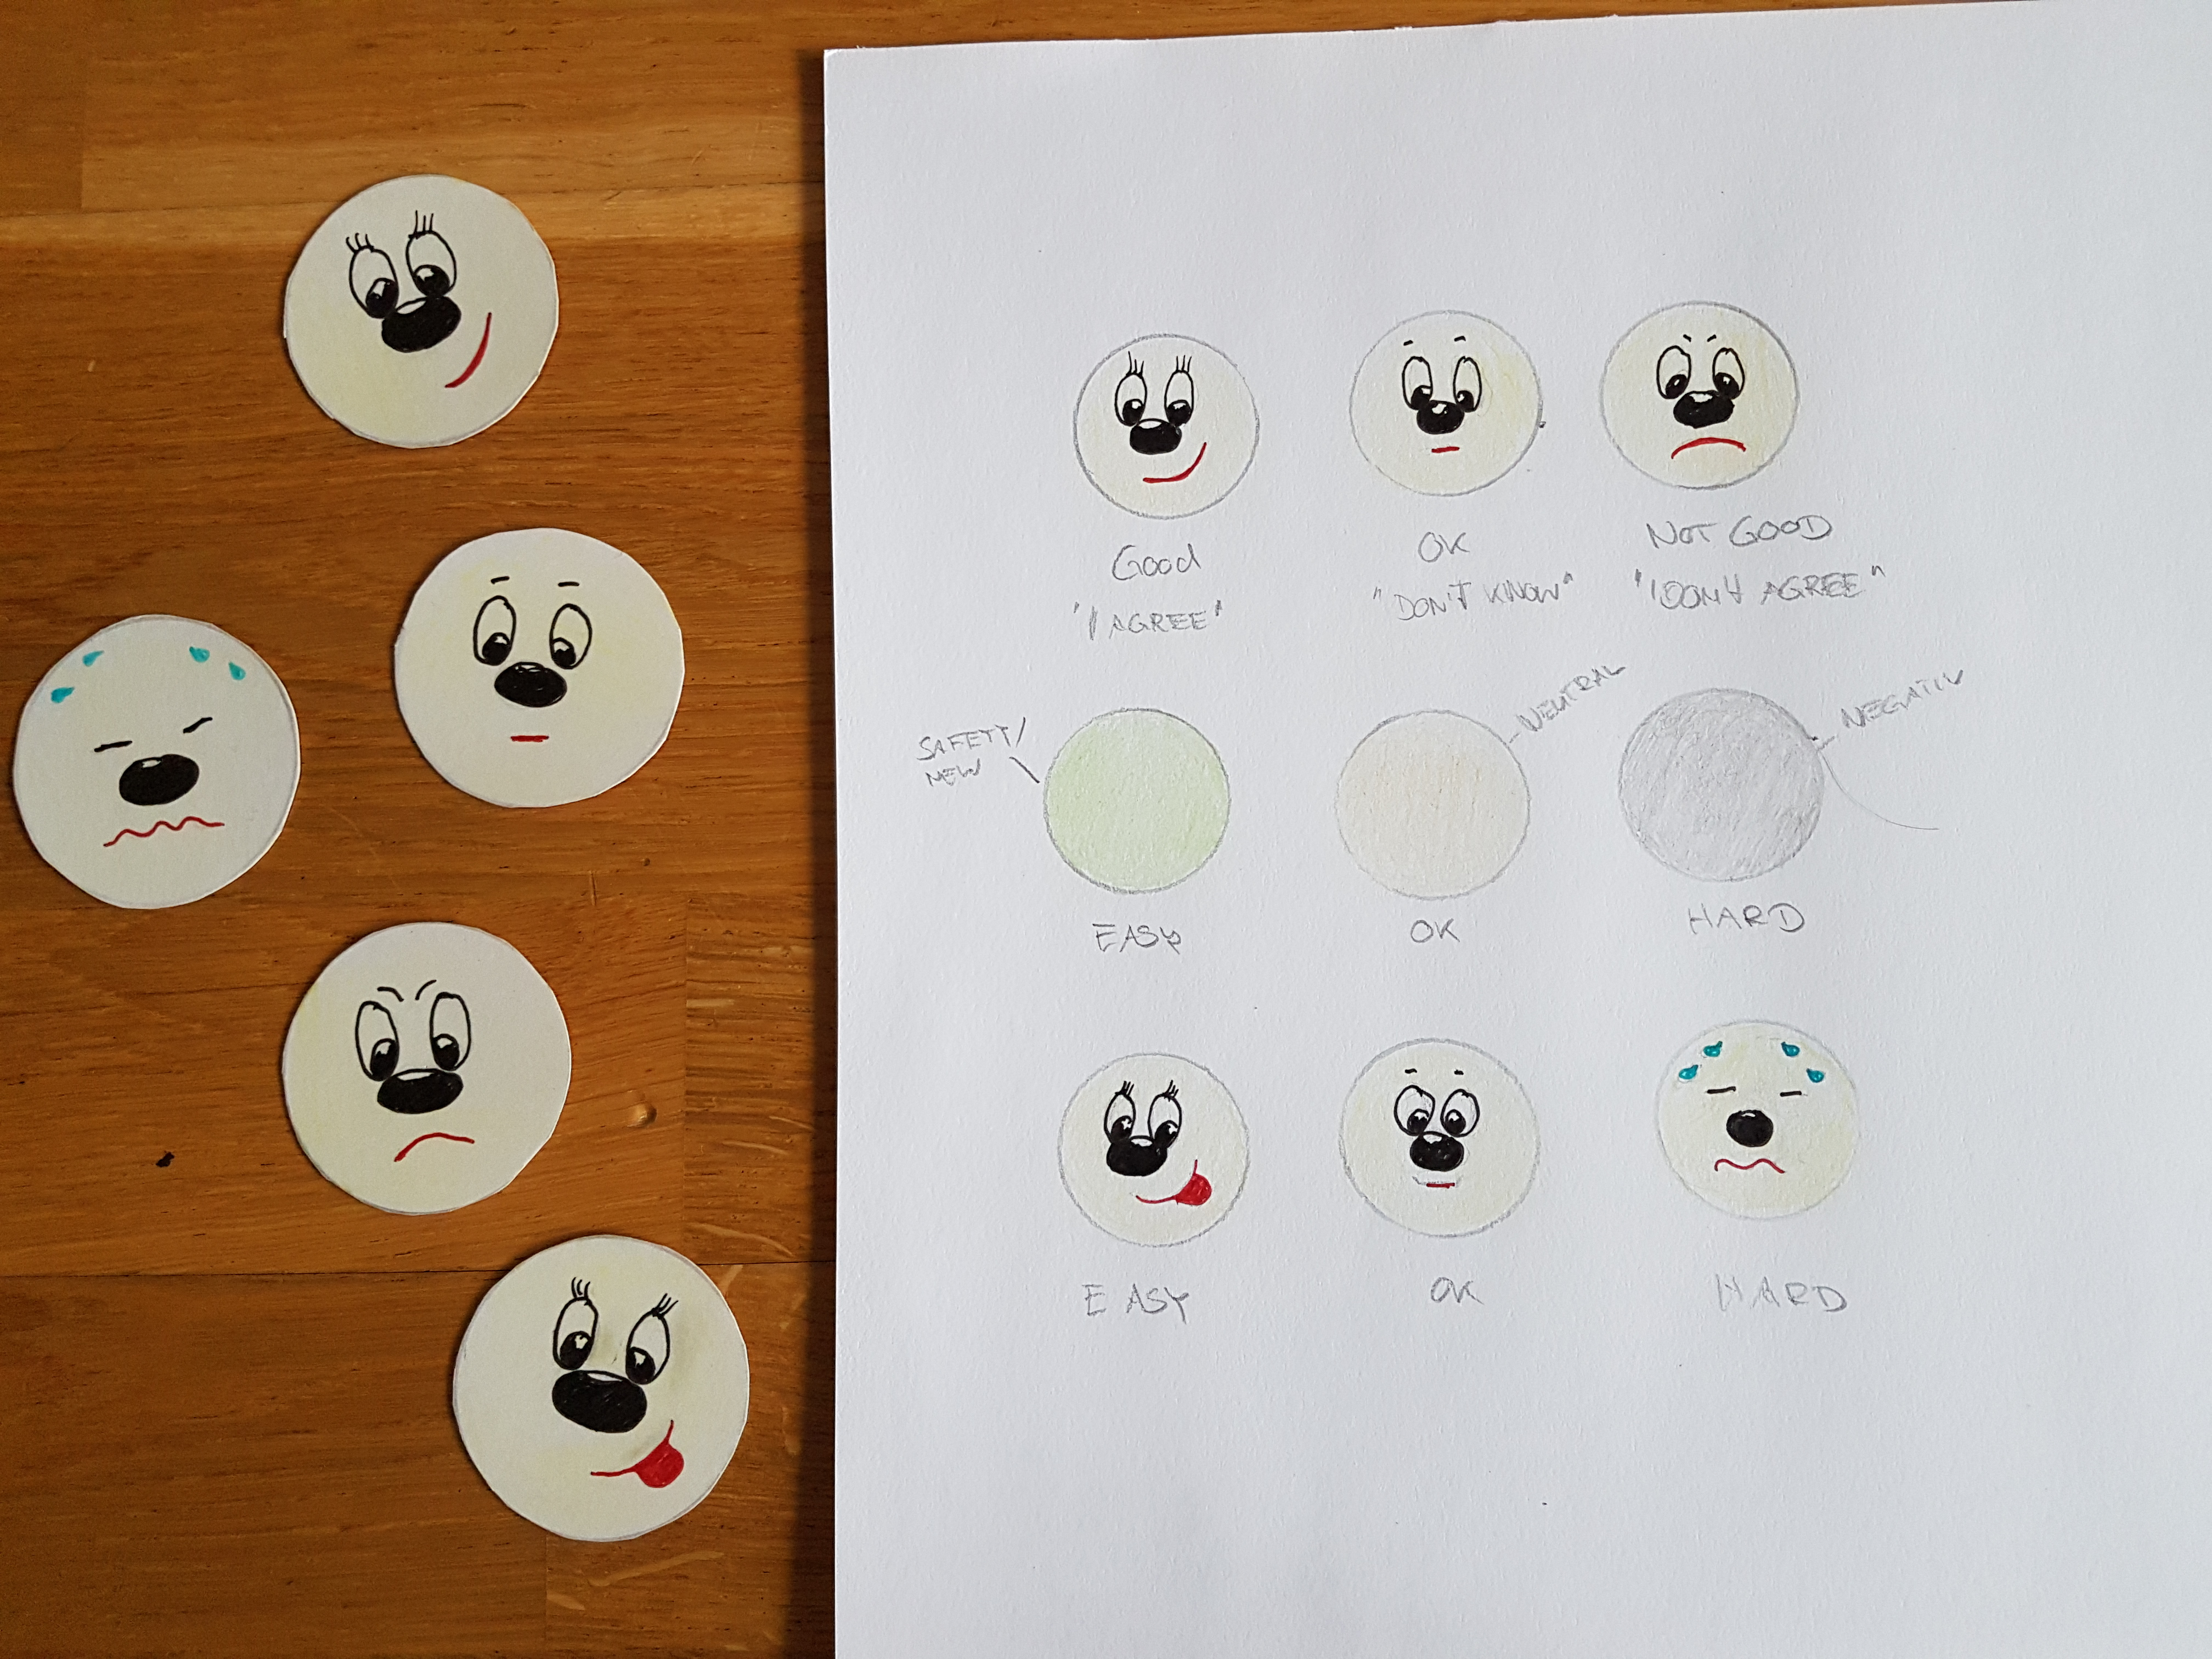
\includegraphics[width=.5\textwidth]{figures/scale.jpg}
  \caption[Visual scale.]{Visual scale.}
  \label{fig:setup}
\end{figure}

The gathered information and data is evaluated and presented in chapter~\ref{chap:dataanalysis} and will be further discussed in chapter~\ref{chap:discussion}.

(see attached questionnaire in the the attachment section.)



\section{Observations}

Observation is a common scientific method and often used in research projects.[reference] 
Observation during this experiment focused on the child's behaviour and reaction during the experiment. Additionally,the ability to perform the task and how much assistance was needed was recorded.
%\chapter{Data analysis  and presentation of data}
\label{chap:dataanalysis}

%kids > curious about leap motion. "what is that thing" > seemed to be interrested
\chapter{Data presentation and analysis}
\label{chap:dataanalysis}

The prove of principle type of review was carried out on 8 from 10 planed participants. The number of participants was decreased because all information that was needed for further evaluation was already gather at this point and more test persons would not provide any new relevant data. Furthermore, the usability experiment focused more on gathering qualitative data than on quantitative data collection. Additionally, the youngest participant was three years old which deviates from the planed minimum age of two years. During the test sessions it turned out that the four and three years old participants already struggled to carry out the task which led to the conclusion that a toddler of two years of age would not have the expected understanding and motor development. The age and gender distribution of the prove of principle type of review is presented visually in table \ref{tab:participanttable}. Each participant was right handed and had no previous experience with hand-free gesture based games.


%all were right handed and novice users

\renewcommand{\arraystretch}{1.5}
 \begin{table}[h]
     \centering
     \begin{tabular}{c|c|c|c|c|c|c|c}
     \hline
        \multicolumn{1}{|l|}{\textbf{AGE:}}  &
        \multicolumn{1}{l|}{3}  &     
        \multicolumn{1}{l|}{4}  & 
        \multicolumn{1}{l|}{5}  & 
        \multicolumn{1}{l|}{7}  & 
        \multicolumn{1}{l|}{8}  & 
        \multicolumn{1}{l|}{9}  & 
        \multicolumn{1}{l|}{13} \\ \hline
        \multicolumn{1}{|l|}{\textbf{AMOUNT:}} &
        \multicolumn{1}{l|}{1}  &
        \multicolumn{1}{l|}{1}  &
        \multicolumn{1}{l|}{1}  &
        \multicolumn{1}{l|}{2}  &
        \multicolumn{1}{l|}{1}  &
        \multicolumn{1}{l|}{1}  &
        \multicolumn{1}{l|}{1}  \\ \hline
        \multicolumn{1}{|l|}{\textbf{GENDER:}}  &
        \multicolumn{1}{|l|}{F} &
        \multicolumn{1}{l|}{M}  &
        \multicolumn{1}{l|}{M}  &
        \multicolumn{1}{l|}{F/M}&
        \multicolumn{1}{l|}{F}  &
        \multicolumn{1}{l|}{M}  &
        \multicolumn{1}{l|}{F}  \\ \hline
        \multicolumn{1}{|l|}{\textbf{L/R HANDED:}} &
        \multicolumn{1}{|l|}{R} &
        \multicolumn{1}{l|}{R}  &
        \multicolumn{1}{l|}{R}  &
        \multicolumn{1}{l|}{R}  &
        \multicolumn{1}{l|}{R}  &
        \multicolumn{1}{l|}{R}  &
        \multicolumn{1}{l|}{R}  \\ \hline
        \multicolumn{1}{|l|}{\textbf{NOVICE/EXPERT:}} &
        \multicolumn{1}{|l|}{N} &
        \multicolumn{1}{l|}{N}  &
        \multicolumn{1}{l|}{N}  &
        \multicolumn{1}{l|}{N}  &
        \multicolumn{1}{l|}{N}  &
        \multicolumn{1}{l|}{N}  &
        \multicolumn{1}{l|}{N}  \\ \hline
     \end{tabular}
     \caption{Presentation of participants}
     \label{tab:participanttable}
 \end{table}
 

The age of the participant ranged from three to 13 years and included a mixture of boys and girls. 50\texttt{\%} boys and 50\texttt{\%} girls was a good balanced gender distribution. An equal distribution of gender is crucial when doing scientific research, since both genders have its own distinct characteristics. The age that most frequently appeared (mode) in this sample is 7. The arithmetic average age of the sample (mean) is also 7 and the standard deviation of the sample is 2,96 (Table \ref{tab:agestatistic}).
%Regarding the age distribution, table  \ref{tab:agestatistic} presents a statistical calculation for age distribution of the sample in this study. 
%It shows that the average age of the sample (mean) is 7 and the standard deviation of the sample is 2,96.
Additionally, the statistical calculation revealed that 87,5 \texttt{\%} of the participant finished the game at the first attempt which indicates that the game was challenging but not impossible (Figure \ref{fig:finishedgame}). 


\renewcommand{\arraystretch}{1.5}

\begin{table}[!ht]
    \centering
    \begin{tabular}{c|c|c|c}
    \hline
        \multicolumn{1}{|c|}{MEAN} &
        \multicolumn{1}{c|}{MEDIAN} &
        \multicolumn{1}{c|}{MODE} &
        \multicolumn{1}{c|}{STANDARD DEVIATION}\\ \hline
       \multicolumn{1}{|c|}{7} &
        \multicolumn{1}{c|}{7} &
        \multicolumn{1}{c|}{7} &
        \multicolumn{1}{c|}{2,96} \\ \hline
    \end{tabular}
    \caption{Average age of participants}
    \label{tab:agestatistic}
\end{table}


\begin{figure}[!ht]
   \centering
    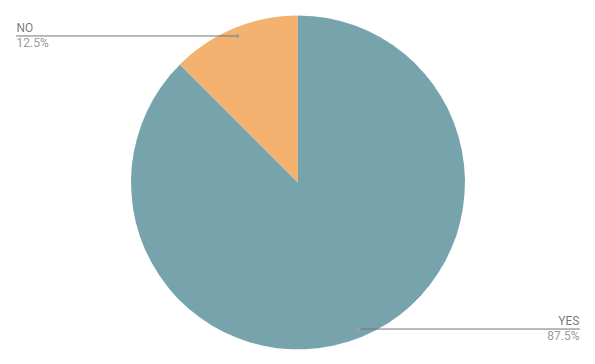
\includegraphics[width=.4\textwidth]{figures/finishedgame.png}
    \caption{Percentage of children who finished the game}
    \label{fig:finishedgame}
\end{figure}

\newpage


\section{Ability test data and questionnaire}
The primary parameters in the ability test are \textit{time} and \textit{hits} (precision) where time is in relation to hits. The less time needed to finished the game and the more precise navigation of the mole figure the better.
The closed-end questionnaire was scaled with good-ok-bad and easy-ok-hard. This scale was converted into digits where good/easy represents number 1, ok represents number 2 and bad/hard represents number 3 (Table \ref{tab:closedendedquestions}).
Sometimes, a participant did not want to answer the question (NA) or did not know (NK) the answer of a question. Since this study is based on voluntary and all compulsion could bias the outcome, the children were never force to respond to a question if they did not want to.

By inspecting the data as a whole, a global relation between entity could so be illustrated. The investigation of the relation between time and age group by using SPSS, a software for statistical analysis and data management, revealed a connection between age and finishing time. The participants were divided into three groups in order to ensure a better visual presentation of the outcome. Group one included participants from age three to age five, group two included participants from age seven to age eight, and participant from age nine to age 13 were placed in group 3.

The analyzed age-time data showed that group three had the best result in regard to the time score. They finished the task in the shortest time. 
Players in group one needed the longest time to finish the game which can be explained by their least developed motor skills. Due to the fact that the finish-time decreases with age, it suggest a relation between age and improved eye-hand coordination and increased fine motor performance (Figure \ref{fig:relationTimeAge}).

Two of the participants had a lot of hit-points at their last attempt which implies an inpatient behavior and the desire to finish the game as fast as possible. On the other hand, two other participants did improve both time and precision at the last attempt. Again, this could be explained by the child's personality and the willingness to do best. However, increased performance can also be a result of a learning effect.

Moreover, participants \texttt{\#}3, \texttt{\#}6 pointed out that the task and stabilizing of the hand was most difficult. According to the data from table \ref{tab:closedendedquestions} the older participants did not have any difficulties or experienced any fatigue regarding the midair hand position when playing the game. Furthermore, none of them had strong opinions on the difficulty level of the task, they found it manageable. The result implies a relation between age and midair hand positing. The older the participant the easier midair hand position and the execution of free-hand tasks (Figure \ref{fig:Q1}, \ref{fig:Q3}, \ref{fig:Q4}). 


Participants \texttt{\#}2, \texttt{\#}4 and \texttt{\#}5 replied to the closed-end questions (Table \ref{tab:closedendedquestions}) \textit{"safely"}. They did not have any strong opinions regarding difficulty level or affinity for the game. However, the open-ended questions (Table \ref{tab:openendedquestion}) revealed some more details and impressions. The biggest challenge for those children was to navigate the pointer and to stay in the allowed area.  

Moreover, participant \texttt{\#} 7 executed only two of three attempts. It seemed that he got bored when he found out that the game just was a prototype and that he could cheat the system, something he also pointed out in the follow up questions and conversation. (The values of his second attempt is a result of going directly from start to finish.)


An interestingly statement was made by participants \texttt{\#}1, \texttt{\#}5. They pointed out that not to touch the screen in order to control the game was problematic. This could be explained due to the unfamiliarity of touch-less navigation.

Regarding the game design and enjoyment, the participants revealed a great sympathy for the game (Figure \ref{fig:Q5}).
To the question what they like the most about the game, they pointed out the mole figure.

The result of participant \texttt{\#}3 and \texttt{\#}8 confirmed that touch-less gesture based interactions need certain motor skills, conceptual and spatial understanding of the touch-free concept (Figure \ref{fig:agegroup1}).The ability test demonstrated that these skills are not ensured in children younger than 4.

\section{Observational data}
During the ability test, the children were closely observed in order to gather information about how they handled the situation, expressed their feelings and coped with the game. Furthermore, some kids are not able to express themselves in words or get stressed when they have to replay a question. For that reason an observation could provide additional information.
There were observed several interesting issues relating to the touch-less concept. The youngest participants had too small fingers which gave them a big disadvantage when playing the game because the sensor did not recognized the stretched finger pose. They belonged to the group (\textit{group 1}) who at least understood the touch-less concept. They wanted to touched the screen in order to move the pointer or the mole. 
Most of the children were very curious about the Leap Motion sensor. They called it "the thing" because they never had seen something like that before. However, almost all of them were very eager to try the game. Especially the boys liked the idea of playing a touch-less game.
Unfortunately, not every child was patient enough. One participant was observed waving her hands and impatiently trying to make the pointer move to the mole. She also supported the pointing hand with her other hand, not because it was tiring to hold the hand above the device but rather as a help to navigate the finger in the right direction.  
Furthermore, the observation revealed that the most difficult gesture action during the sessions was the poking gesture. The game demanded a poking action in order to activate the walking mole.
Moreover, some users were very concentrated and focused on doing the task right. However they forgot about the right gesture, namely the poking finger. The finger needed to be completely stretched so the sensor could recognize the gesture. The consequence of the relaxed finger was that the system had trouble to distinguish the gesture.

Unfortunately, the prototype had some technical issues. The kids found out that it was possible to fool the system by directly going from start to finished without following the tunnel. Some other issues regarding time, hits and movement were observed as well. 


\begin{figure}[!ht]
    \centering
    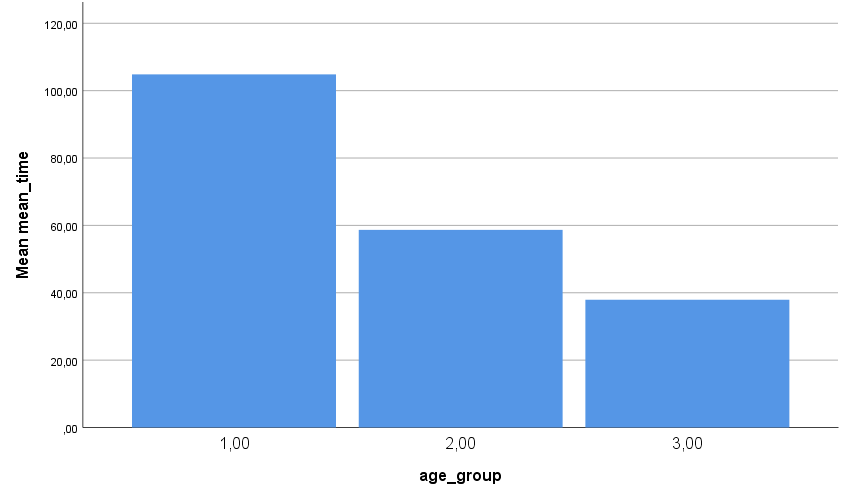
\includegraphics[width=.6\textwidth]{figures/relationTimeAge.png}
    \caption{Relation between age and time}
    \label{fig:relationTimeAge}
\end{figure}

\begin{figure}[!ht]
    \centering
    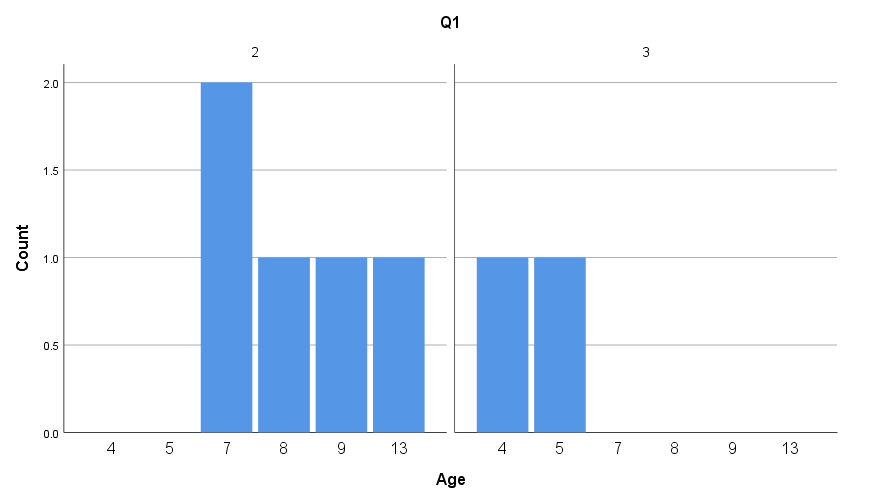
\includegraphics[width=.6\textwidth]{figures/Q1.png}
    \caption{Graphical presentation of question 1: Task difficulty}
    \label{fig:Q1}
\end{figure}
\begin{figure}[!ht]
    \centering
    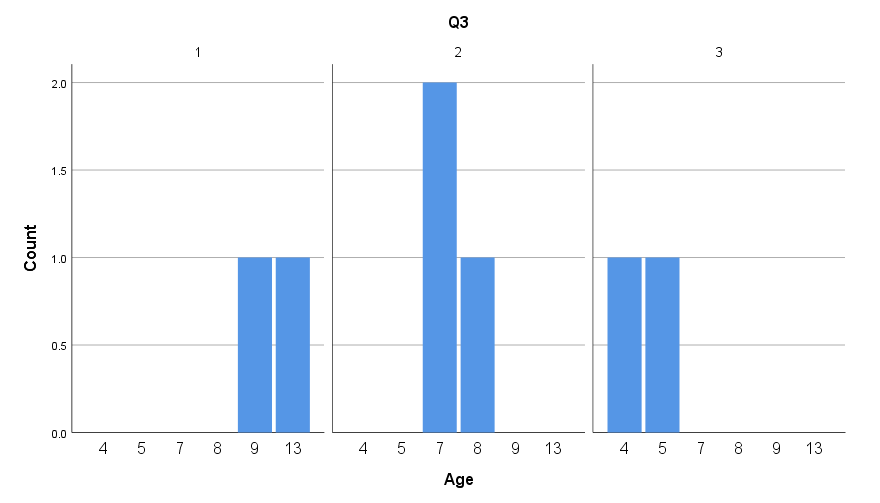
\includegraphics[width=.6\textwidth]{figures/Q3.png}
    \caption{Graphical presentation of question 3: Hand stabilization difficulty}
    \label{fig:Q3}
\end{figure}
\begin{figure}[!ht]
    \centering
    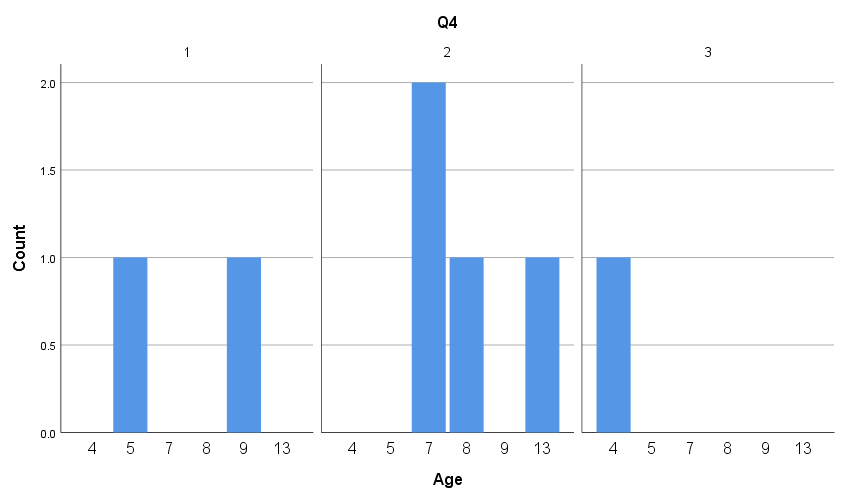
\includegraphics[width=.6\textwidth]{figures/Q4.png}
    \caption{Graphical presentation of question 4: Gesture and navigation difficulty}
    \label{fig:Q4}
\end{figure}
\begin{figure}[!ht]
    \centering
    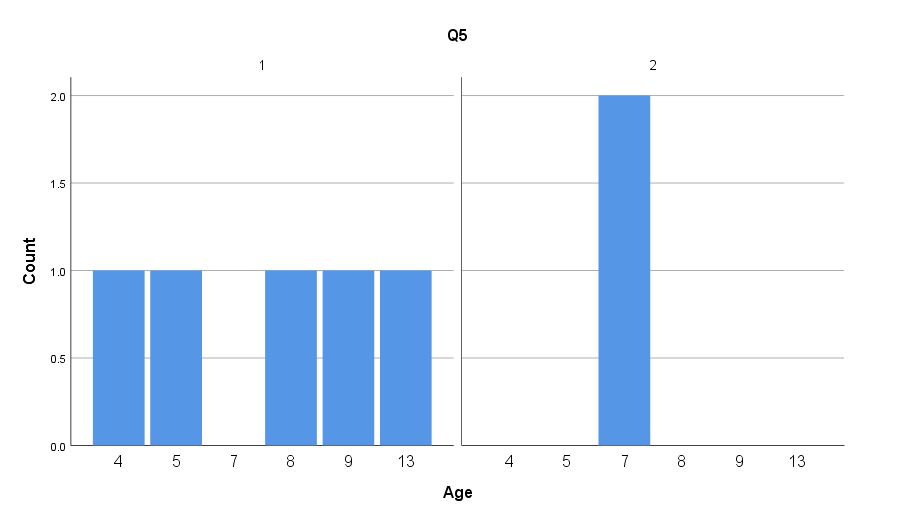
\includegraphics[width=.6\textwidth]{figures/Q5.png}
    \caption{Graphical presentation of question 5: Game sympathy }
    \label{fig:Q5}
\end{figure}



\begin{table}[!ht]
    \centering
    \begin{tabular}{c|c|c|c|c}
    \hline
    \multicolumn{1}{|c|}{\textbf{Question/participant}} &
    \multicolumn{1}{c|}{\textbf{Q1}} &
    \multicolumn{1}{c|}{\textbf{Q3}} &
    \multicolumn{1}{c|}{\textbf{Q4}} &
    \multicolumn{1}{c|}{\textbf{Q5}} \\ \hline
 
    \multicolumn{1}{|c|}{\textbf{P\texttt{\#}3}} &
    \multicolumn{1}{c|}{3} &
    \multicolumn{1}{c|}{3} &
    \multicolumn{1}{c|}{3} &
    \multicolumn{1}{c|}{1} \\ \hline
    \multicolumn{1}{|c|}{\textbf{P\texttt{\#}6}} &
    \multicolumn{1}{c|}{3} &
    \multicolumn{1}{c|}{3} &
    \multicolumn{1}{c|}{1} &
    \multicolumn{1}{c|}{1} \\ \hline
    \multicolumn{1}{|c|}{\textbf{P\texttt{\#}8}} &
    \multicolumn{1}{c|}{-} &
    \multicolumn{1}{c|}{-} &
    \multicolumn{1}{c|}{-} &
    \multicolumn{1}{c|}{-} \\ \hline
    \multicolumn{1}{|c|}{\textbf{P\texttt{\#}2}} &
    \multicolumn{1}{c|}{2} &
    \multicolumn{1}{c|}{2} &
    \multicolumn{1}{c|}{2} &
    \multicolumn{1}{c|}{1} \\ \hline
    \multicolumn{1}{|c|}{\textbf{P\texttt{\#}4}} &
    \multicolumn{1}{c|}{2} &
    \multicolumn{1}{c|}{2} &
    \multicolumn{1}{c|}{2} &
    \multicolumn{1}{c|}{2} \\ \hline
    \multicolumn{1}{|c|}{\textbf{P\texttt{\#}5}} &
    \multicolumn{1}{c|}{2} &
    \multicolumn{1}{c|}{2} &
    \multicolumn{1}{c|}{2} &
    \multicolumn{1}{c|}{2} \\ \hline
    \multicolumn{1}{|c|}{\textbf{P\texttt{\#}1}} &
    \multicolumn{1}{c|}{2} &
    \multicolumn{1}{c|}{1} &
    \multicolumn{1}{c|}{2} &
    \multicolumn{1}{c|}{1} \\ \hline
    \multicolumn{1}{|c|}{\textbf{P\texttt{\#}7}} &
    \multicolumn{1}{c|}{2} &
    \multicolumn{1}{c|}{1} &
    \multicolumn{1}{c|}{1} &
    \multicolumn{1}{c|}{2} \\ \hline
    \end{tabular}
    \caption{Closed-ended questions}
    \label{tab:closedendedquestions}
\end{table}


\begin{table}[!ht]
    \centering
    \begin{tabular}{c|c|c|c|c}
    \hline
  %  \rowcolor{1}{green}
    \multicolumn{1}{|c|}{\textbf{Question/participant}} &
    \multicolumn{1}{c|}{\textbf{Q2}} &
    \multicolumn{1}{c|}{\textbf{Q6}} &
    \multicolumn{1}{c|}{\textbf{Q7}} &
    \multicolumn{1}{c|}{\textbf{Q8}} \\ \hline
    \multicolumn{1}{|c|}{\textbf{P\texttt{\#}3}} &
    \multicolumn{1}{c|}{NK} &
    \multicolumn{1}{c|}{mole} &
    \multicolumn{1}{c|}{NA} &
    \multicolumn{1}{c|}{NA} \\ \hline
    \multicolumn{1}{|c|}{\textbf{P\texttt{\#}6}} &
    \multicolumn{1}{c|}{NA} &
    \multicolumn{1}{c|}{mole} &
    \multicolumn{1}{c|}{navigate - pointer} &
    \multicolumn{1}{c|}{OK} \\ \hline
    \multicolumn{1}{|c|}{\textbf{P\texttt{\#}8}} &
    \multicolumn{1}{c|}{-} &
    \multicolumn{1}{c|}{-} &
    \multicolumn{1}{c|}{-} &
    \multicolumn{1}{c|}{-} \\ \hline
        \multicolumn{1}{|c|}{\textbf{P\texttt{\#}2}} &
    \multicolumn{1}{c|}{not to cross the line} &
    \multicolumn{1}{c|}{NA} &
    \multicolumn{1}{c|}{NA} &
    \multicolumn{1}{c|}{OK} \\ \hline
    \multicolumn{1}{|c|}{\textbf{P\texttt{\#}4}} &
    \multicolumn{1}{c|}{to move the pointer} &
    \multicolumn{1}{c|}{follow the white path} &
    \multicolumn{1}{c|}{navigate - pointer} &
    \multicolumn{1}{c|}{OK} \\ \hline
    \multicolumn{1}{|c|}{\textbf{P\texttt{\#}5}} &
    \multicolumn{1}{c|}{not to touch the screen} &
    \multicolumn{1}{c|}{NA} &
    \multicolumn{1}{c|}{NA} &
    \multicolumn{1}{c|}{OK} \\ \hline
       \multicolumn{1}{|c|}{\textbf{P\texttt{\#}1}} &
    \multicolumn{1}{c|}{not to touch the screen} &
    \multicolumn{1}{c|}{NA} &
    \multicolumn{1}{c|}{NA} &
    \multicolumn{1}{c|}{OK} \\ \hline
    \multicolumn{1}{|c|}{\textbf{P\texttt{\#}7}} &
    \multicolumn{1}{c|}{stay in tunnel} &
    \multicolumn{1}{c|}{challenging} &
    \multicolumn{1}{c|}{uncontrolled mole} &
    \multicolumn{1}{c|}{OK} \\ \hline
    \end{tabular}
    \caption{Open-ended questions}
    \label{tab:openendedquestion}
\end{table}





\begin{figure}[!ht]

    \centering
    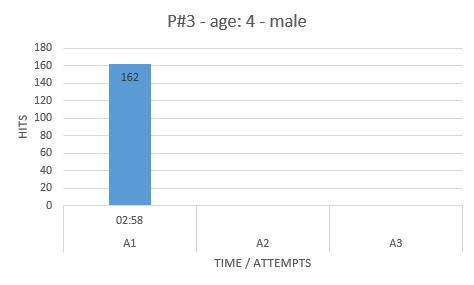
\includegraphics[width=.6\textwidth]{figures/p3.png}
   %  \caption{Participant \texttt{\#}3}
    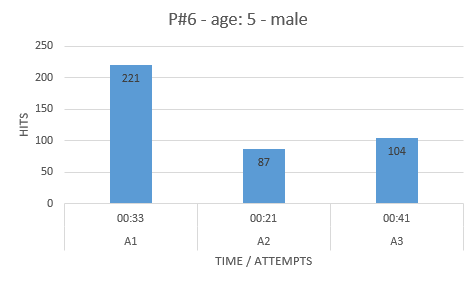
\includegraphics[width=.6\textwidth]{figures/p6.png}
 %   \caption{Participant \texttt{\#}6}
        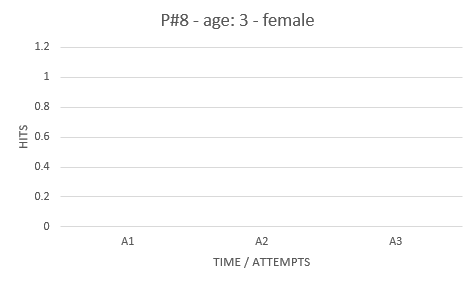
\includegraphics[width=.6\textwidth]{figures/p8.png}
    \caption{Time/hit parameters. Data presentation of group 1. Participants \texttt{\#}3, 6 and 8}
    \label{fig:agegroup1}
\end{figure}

\begin{figure}[!ht]
    \centering
    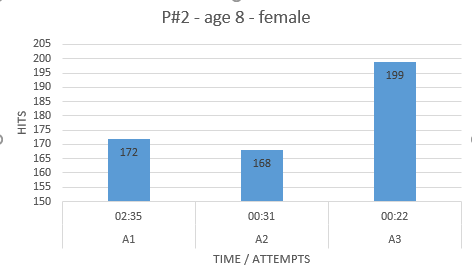
\includegraphics[width=.6\textwidth]{figures/p2.png}
    % \caption{Participant \texttt{\#}2}
    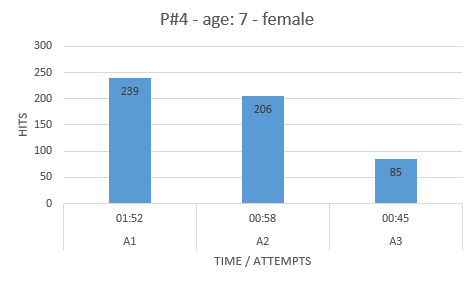
\includegraphics[width=.6\textwidth]{figures/p4.png}
   % \caption{Participant \texttt{\#}4}
        \includegraphics[width=.6\textwidth]{figures/p5.png}
    \caption{Time/hit parameters. Data presentation of group 2. Participants \texttt{\#}2, 4 and 5}
    \label{fig:agegroup2}
\end{figure}

\begin{figure}[!ht]
    \centering
    \includegraphics[width=.6\textwidth]{figures/p1.png}
     %\caption{Participant \texttt{\#}1}
    \includegraphics[width=.6\textwidth]{figures/p7.png}
    \caption{Time/hit parameters. Data presentation of group 3. Participants \texttt{\#}1 and 7}

    \label{fig:agegroup3}
\end{figure}






%\chapter{Result}
\label{chap:result}

\chapter{Discussion}
\label{chap:discussion}
%theory
%data
%proving the argument

%best age group
%the deviation of time and hit was as expected varying. the study was not about reliable parameter but if it is possible to gather parameters. since the game just was a prototype the result was expected not to be reliable

%She also supported the pointing hand with her other hand, not because it was hard to hold the hand up but rather to help the finger in the right direction. Something like that could be used to point to a hand-eye coordination issue.

%critical exam findings
%contribution
%compare with other work, facts
%make a knowledge claim
%observation backup with evidence
%any unexpected findings
% weaknes of the study , eks choice and amount of particiant , bad code, inexperience interviewer, 

%validity + reliability

%can not be used to determine early stage of ASD > refer age of child in test

%Earlier, we pointed out that....However...
%paramenters + observation > ASD

The literature review, pointed out that designing gestural touch-less interfaces demand guidelines and an understanding of the challenges it arises (Norman Nielsen 2010, Malixia, Montero 2010). Researcher are two minded whether gestural interaction is natural and in what extent it is a convenient form for interacting with computer and other systems(Montero 2010, Maliza2012, Norman 2010, Park 2013, riener 2012). Other argue, that gesture interfaces are stimulating and enjoyable (Loehnman 2013, Ren 2013) Moreover, navigating precisely in free space is argued as a big disadvantage when dealing with gesture interfaces (Ni et al, 2011, Siek, Roger, Conelley).

The analyzed data presented in the previous chapter revealed some interesting findings that shows a clear correlation between the literature review and the prove of principle type of review. Although the gathered data corresponds to a small sample of the population it provided valuable knowledge about hand-free gesture based screening systems. As Norman, Nielsen and co stated, gesture based interaction need guidelines and do not come natural if the user never needed to deal with this kind of interaction. The children in this study would not know how to play the game if it had not been showed them. They never had seen this kind of interaction before and for that reason could not build a conceptual model of the system (Norman, 2002). However, if gesture interaction would be more usual such as touch based gesture interaction than it would be more know and more natural to people. Nevertheless, without guidelines that define what type of gesture trigger a certain action, it would be a challenging form of interaction for all unknown systems. 
The study also confirmed that gesture interfaces offers a pleasurable experience (Loehnman, REn). The children valued the games highly which also was observed by their body language during the task. 
The problem with navigating in free space as Ni and Siek argued, can be confirmed only partly. The study showed that users who have not a fully developed fine motor ability such as in toddlers and very young children have experienced such challenge. However, the fine motor ability increases with age (Figure \ref{fig:relationTimeAge}). Nevertheless, it can not be ruled out that people with fine motor deficit or eye - hand coordination deficit will also experience problems with navigating precisely since such task demand high fine motor performance. This assertion can be confirmed by the observation of a participant that needed to support her pointing hand in order to be more precisely in her navigation and pointing action. 

As suggested in chapter \ref{chap:aim}, figure \ref{fig:tableOfModules}, the main parameters to be extracted from the game Mole in the hole were time - needed to finish the game and number of hits - path deviation. The secondary parameters where touchzone and pointable extended. 
%ikke strekke > konsentrasjons ?






\section{Limitation}

%what is left out, yet to-do

\chapter{Conclusion}
\label{chap:conclusion}

%used as a complementary /supplementary tool 

%Proof of concept (PoC) is a realization of a certain method or idea in order to demonstrate its feasibility

%Re-introduce the project and the need for the work
%Re-iterate the purpose and specific objectives of your project
%Re-cap the approach taken
%Summarize the major findings
%recommendations of your work

Free-hand gesture interaction with computer system and interfaces is a relative new modality. This field is of growing interest not only because it is an enjoyable kind of interaction but it is also important when visual focus is needed. Some researcher argue that free-hand gesture interaction is convenient for manipulating systems because gestures are natural to human. Gestures are used in humans daily behaviour, for instance by saying goodbye, ok or pointing at something. 
Free-hand gesture interfaces are already employed in industry and in health care (Grundmann, 2016). However, using free-hand gesture in a screening type of method is still little explored.

The concept of this study was to examine an idea about using Leap Motion and free-hand gesture interaction in order to measure motor performance in children. This was a prove of principle kind of approach where the specific idea was checked for its feasibility. Thus, the goal was to investigate the feasibility of using Leap Motion controller to extract motor performance parameters. Since there is only few research in this field, the value of project was significant.

In order to prove the concept and investigate possibilities, a simple prototype was created in Processing, an open source computer language. This program was established mainly for electronic art and visual design but it is suitable for prototyping as well. Processing was a convenient prototype tool for this project since it is build on Java programming language and most important because of its compatibility to Leap Motion. Using Leap motion as a motion sensor tool was well-chosen due it economical benefits and the fact that it could record finger and hand gestures.\\
At the beginning of the project, interviews in form of a brief conversation were carried out to ascertain existing screening method for motor performance and the fact that it could be used to determine Autism. Autism was pointed out as an example to illustrate what kind of disorder could be detected by applying the free-hand gesture concept. The inspiration for the concept was based on an existing motor coordination test called Movement Assessment Battery for Children (MABC-2) which is a standard performance test that includes specific motor exercises.  
Ideas from the MABC-2 were used to create a concept that included a collection of five mini games. However, to implement and investigate these five games would be beyond the scope of this project. Thus, only one games was selected and chosen to be implemented further. "Mole in the hole" is a free-hand gesture based game where the player must guide the mole through its tunnel on the way out. During the game parameters such as time and accuracy were recorded. The goal of the game was to move the mole as fast as possible and to be accurate as much as possible.
The game was tested on 8 children, the youngest child was 3 years of age and the oldest child was 13 years of age. The test showed that children under 5 did not understand the free-hand concept. They constantly touched the screen in order to move the mole. Moreover, the sensor had problems to detect gestures from toddlers due to the tiny size of the finger and the vague gestures. Consequently, this method is not applicable on children younger than 5 years old. 
Furthermore, observation revealed that all children showed interest in the game and enjoyed the free-hand concept which could be explained by the fact that none of them had pre-experience in free-hand gesture interactions. It seemed that an appealing interface has a great impact on how children react to serious games like suggested in this project. The children were pointing out the mole figure as the most liked element in the game. 
%sag noch was zu ASD

To sum up, the study demonstrated that it is possible to extract motor performance parameters, such as time and accuracy, from a Leap Motion driven computer game. However, it is not possible to apply these kind of screening method on toddlers since their motor performance skills are not enough developed and they do not have a conceptual understanding of the free-hand concept. Additionally, tiny fingers and vague gesture were the reason why the sensor had problems to detect gestures from toddlers.
Moreover, using the freehand gesture concept as a stand alone screening method is not advisable. As the interview with the pediatrician confirmed, it should be used as a supplementary tool in a more complex screening procedure. Due to the fact that this method provides objective data, it could be a valuable tool to determine developmental disorder.  



\section{Future Work}
\label{sec:future}
%Make recommendations for future research
%test mot autisme
%test med flere personer
%lage flere tester
%Base on the experience of this study , the following recommendation can be presented
%what is left out, yet to-do
%Due to the limited time scope of this study, many interesting points needed to be left out.


The information and experience gained during this study is a great point of departure for further exploration and research.  
Firstly, it is recommended to improve the prototype and to do extensive testing on more children with a broader age rage and a more spread sample. Secondly, it can be a good idea to implement the other games suggested in this study in order to provide varied test methods.
Moreover, further investigation whether this is a suitable screening method for determining Autism in children would have been beneficial. This can be done for instance by sampling a two test groups. One group samples children with Autism and the other group non-autistic children. The result of those group could than have been compared and analyzed. 
Beside testing this concept for screening method it could be also interesting to explore whether free-hand gesture interactions is suitable as a therapy tool for neurological injuries. That could be either in form of a PC game or combined with Arduino. The idea is to navigate an Auduino car with specific gestures in order to enhance hand mobility.  


%test for theray tool
%test with arduino
%make a better prototype and test more children
%test with children som har et motor problem


%first of all


\ifthenelse{\boolean{HarvardCitations}}{%
	\bibliographystyle{agsm} % used for Harvard style references. Names - Humanities & Interaction Design
}{%
	\bibliographystyle{ntnuthesis/ntnuthesis} %used for Vancover style references. Numbers - Computer Science & Physics
}

\bibliography{MyBibLibrary}

\appendix
\chapter{Testing Data}
This could be a log of the testing sessions and raw data that is too long for the thesis.
\section{Test Session 1}
\subsection*{Objective}
The Objective of this testing session was to test Hypothesis ....

\subsection*{Participants}
The participants were a convenience sample of students from NTNU. Age range $19-55$ Median age $23$ ...


\subsection{Raw Data}





%\includepdf[pages=1]{figures/consentformminor}
\chapter{Appendix - Ability-Test Form}





%\include{inc/timetable}
\includepdf[pages=1]{figures/AgilityTestPage1}
\includepdf[pages=1]{figures/AgilityTestPage2}
\chapter{Appendix - Processing Code}

\lstset{language=Java}
\begin{lstlisting}[caption = {}, label={lst:Java}]
import com.leapmotion.leap.*;
Controller leap;
PImage backgroundImage;
PImage MoleState1;
PImage MoleState2;
PImage MoleJump;
PImage MoleGo;
PImage MoleKaBoom;
PImage Timer;
PShape pointer;
int cols, rows;
int w = 80;
int [] grid; //one dimension array
int windowWidth = 1200;
int windowHeight = 800;
int state = 0;
int [][] gridArray = new int [15][10];
int countOK = 0;
int countKaBoom = 0;
int stateEnd = 0;
int counterState = 0; //status for timer
int counterTouching =0;

void setup()
{
  size(1200, 800);//(1440, 960);
  
  backgroundImage = loadImage("Mole-in-the-hole-800x1200-GRIDinBack.jpg");
  backgroundImage.resize(1200, 800);
  MoleState1= loadImage("MoleState1.png");
  MoleState2= loadImage("MoleState2.png");
  MoleJump = loadImage("MoleJump.png");
  MoleGo = loadImage("MoleGo.png");
  MoleKaBoom = loadImage("MoleKaBoom.png");
  Timer = loadImage("timer.png");

  pointer = createShape(ELLIPSE, 0, 0, 40, 40);
  pointer.setFill(color(127, 0, 0));

  leap = new Controller();
}
void draw()
{
  background(backgroundImage);

  //KaBoom counter & timer
  CounterKaBoom();
  Timer(0);// state 0 , not startet
  image(MoleKaBoom, 30, 50);
  image(Timer, 30, 150);

  InteractionBox iBox = leap.frame().interactionBox();
  Pointable pointable = leap.frame().pointables().frontmost();

  Vector normalizedPosition = iBox.normalizePoint(pointable.stabilizedTipPosition());
  float pixelX = normalizedPosition.getX() * windowWidth;
  float pixelY = windowHeight - normalizedPosition.getY() * windowHeight;
  int cx = (int) pixelX - 10;
  int cy = (int) pixelY - 100;

  cols = width/w;
  rows = height/w;
  
  Finger finger = new Finger(pointable);
  if(finger.isExtended())
  {
    Timer(1);
  }
  
  //creates grid
  for (int j = 0; j< rows; j++)
  {
    for (int i =0; i< cols; i++)
    {
      int x = i*w;
      int y = j*w;


      Pointable.Zone fingerzone = pointable.touchZone();

      if (state ==0) //state 0 means , do the first block of code - move the pointer to maul and poke him
      {
       if (counterTouching < 5000)//dersom touches are less than x, repeat the following code
        {
         
          shape(pointer, cx, cy);
          
          // println("State3: " + state);   
          if (fingerzone != Pointable.Zone.ZONE_TOUCHING )//start this code if the finger is at 80/480 ((x == 80 && y==480 &&)
          {
            
            show(MoleState1);
          }
          if (cx >=80 && cx <=160 && cy >= 480 && cy <= 560)
          {
            // image(MoleState2, 80, 480);
            switch (pointable.touchZone()) {
            case ZONE_NONE:
              //Handle distant pointable
              image(MoleState1, 80, 480);
              break;
            case ZONE_HOVERING:
              //Handle pointable near touch plane
              hide(MoleState1);
              image(MoleState2, 80, 480);
              break;
            case ZONE_TOUCHING:
              //Handle pointable penetrating touch plane
              //println(count);
              counterTouching = counterTouching + 1;
              image(MoleJump, 80, 480); //mole pic nr 3
               println("touching: " + counterTouching);
             // println("State3: " + state);
              break;
            default:
              //Handle error cases...
              break;
            }//end switch
          }
        
        }
        else//counterTouching is 2 or more
        {
            state = 1;

        }
      }//end if state

    }
  }
  if (state == 1)
  {

    gridArray[1][6] = 1;//start cell
    gridArray[1][5]= 1;//border cell from start cell
    gridArray[1][7]= 1;//border cell from start cell
    gridArray[2][6] = 1;
    gridArray[3][6] = 1;
    gridArray[3][7] = 1;
    gridArray[4][7] = 1;
    gridArray[5][7] = 1;
    gridArray[5][6] = 1;
    gridArray[5][5] = 1;
    gridArray[5][4] = 1;
    gridArray[6][4] = 1;
    gridArray[7][4] = 1;
    gridArray[7][5] = 1;
    gridArray[7][6] = 1;
    gridArray[8][6] = 1;
    gridArray[8][7] = 1;
    gridArray[9][7] = 1;
    gridArray[10][7] = 1;
    gridArray[10][6] = 1;
    gridArray[11][6] = 1;
    gridArray[11][5] = 1;
    gridArray[11][4] = 1;
    gridArray[10][4] = 1;
    gridArray[4][9] = 1;
    gridArray[9][4] = 1;
    gridArray[9][3] = 1;
    gridArray[9][2] = 2;//end Cell

    int coordX = Math.max(Math.min(cx/80, 14), 0);//fixes out of arrayoutofboundary
    int coordY = Math.max(Math.min(cy/80, 9), 0);


    if (coordX == 9 && coordY == 2) // End cell
    {
      countOK++;
      println("TEST"+ coordX + " " +coordY);
      println("HURRRA");
      stateEnd = 1;
      setHide(true, MoleGo);
      image(MoleJump, 720, 160);
      noLoop();
    } else if (gridArray[coordX][coordY] == 1) // Legal
    {
      countOK++;
     // println("OK:" + countOK);
      
      image(MoleGo, cx, cy);
    } else // Illegal
    {
      countKaBoom++;
     // println("KaBOOM:" + countKaBoom);
       image(MoleGo, cx, cy);
    }

    if (stateEnd == 1)
    {
       fill(255, 255, 0);
       text("HURRA!", 600, 200); 
      textColor1();
    }
  }//end state 1
}//end draw


void show(PImage img)
{
  setHide(false, img);
}
void hide(PImage img)
{
  setHide(true, img);
}
void setHide(boolean hideMole, PImage img)
{
  if (hideMole == false && img == MoleState1 )
  {
    image(MoleState1, 80, 480);
  } 
  if (hideMole == false && img == MoleState2 )
  {
    image(MoleState2, 80, 480);
  } 
  if (hideMole == false && img == MoleGo )
  {
    image(MoleGo, 720, 240);
  } else
  {
    hideMole = true;
    //need to hide the mole behind the background.
  }
}

void textColor1()
{
  textSize(100);
  fill(255, 255, 0);
  text("HURRA!", 600, 160); //what is a proper feedback for a child? picture/text
}
void CounterKaBoom()
{

  text("Dunk: " + countKaBoom, 110, 120);
  fill(255, 255, 255);
  textSize(20);
}

void Timer(int startTimer)
{

  if (startTimer == 1)
  {
    int currentMillis = millis();
    setSeconds(currentMillis);
    setMinutes(currentMillis);
  }
  text("Løpetid: " +  getMinutes() +":" +  getSeconds(), 110, 200);
}

int totalSeconds =0;
int totalMinutes  =0;
void setSeconds(int milliseconds)
{
  totalSeconds = (milliseconds / 1000) % 60 ;//millis/1000;
}
int getSeconds()
{
  return totalSeconds;
}
void setMinutes(int milliseconds)
{   
  totalMinutes = ((milliseconds / (1000*60)) % 60);// (seconds/1000)/60;
}
int getMinutes()
{
  return totalMinutes;
}
\end{lstlisting}
\chapter{Appendix - Ability test - Data collection}

\begin{figure}[!ht]
\centering
\includegraphics[width=1\textwidth]{figures/SPSSDATA_simpl.png}
\end{figure}
%[scale=1.2, angle=45]width=0.8\textwidth scale =0.55, angle =90

\end{document}
